\documentclass{book}
\usepackage{latexsym}                % gives us symbols like the diamond
\usepackage{linuxdoc}                % linux documentation style
\usepackage{makeidx}                 % used to make the index
\usepackage{epsfig}                  % I want to include postscript figures
%\usepackage[dvips]{epsfig}           % I want to include postscript figures
\usepackage{float}                   % allows for nicer looking floats
\usepackage[american]{varioref}                % nicer referencing

% these two are for development stuff
%\includeonly{shell2}
\newcommand{\devel}{n} % set to ``y'' or ``n''

% comments that you will see in this document include:
% ``kff:'', starting Karl Fogel's comments
% ``-M'', ending magnuc@ii.uib.no's comments
% ``LG:'', ``-LG'', or nothing usually indicates a comment by me, Larry
%       Greenfield.

% if you're writing, please remember to attribute the comments...

% some macros
\newcommand{\uguide}{{\em The\/ \linux\ Users' Guide\/}}
\newcommand{\ldpgs}{{\em Installation and Getting Started\/}}
\newcommand{\ldpsa}{{\em The\/ \linux\ System Adminstrator's Guide\/}}
\newcommand{\ldpng}{{\em The\/ \linux\ Networking Guide\/}}
% these two are so I can easily add \tm's or change the capitilization
\newcommand{\unix}{Unix}

% index commands
\newcommand{\ttindex}[1]{\index{#1@{\tt #1}}} % gives me a monospaced index
                                              % entry in the correct
                                              % alpha-order...

\newcommand{\bindex}[1]{\index{#1|(}} % this will give a dashed index
                                      % specifier
\newcommand{\eindex}[1]{\index{#1|)}}
\newcommand{\bttindex}[1]{\index{#1@{\tt #1}|(}}
\newcommand{\ettindex}[1]{\index{#1@{\tt #1}|)}}
\newcommand{\impindex}[1]{\index{#1|bold}} % these will print the
                                           % number in boldface
\newcommand{\impttindex}[1]{\index{#1@{\tt #1}|bold}}
\newcommand{\bold}[1]{{\bf #1}} % this is needed for the \imp*index
                                % commands

% this is for the first occurence of a ``concept''
\newcommand{\concept}[1]{{\bf #1}\impindex{#1}\glossary{#1}}

% some new (simple) environments
\newenvironment{command}{\noindent
    \rule{\linewidth}{2pt}\raggedright\large}
  {\\ \rule{\linewidth}{0.5pt}}

\newenvironment{fortune}{\begin{quote}\normalfont\sffamily}{\end{quote}}

% I'm going to redefine \key, because I want a small space after it:
\renewcommand{\key}[1]{\fbox{\sf #1}\,}
\renewcommand{\ret}{\fbox{\sf return}\,}
\newcommand{\eof}{\key{Ctrl-d}} % shortcut like \ret

% change the floatstyle for figure
\floatstyle{ruled}
\restylefloat{figure}

\author{Larry Greenfield} 
\title{The \linux\ Users' Guide}
\years{1993, 1994, 1996}
\abstract{All you need to know to start using \linux, a free \unix\ 
  clone. This manual covers the basic \unix\ commands, as well as the
  more specific \linux\ ones. This manual is intended for the beginning
  \unix\ user, although it may be useful for more experienced users
  for reference purposes.}
% insert the next two when the document is ready:
\if n\devel
   \makeindex
   %\makeglossary
\fi

\begin{document}
% this will give a large ``X'' like the \blackdiamond command.
\newsavebox{\xlogo}
\savebox{\xlogo}{
\epsfig{file=ps-files/xlogo.ps, width=0.5in}}
\def\strutdepth{\dp\strutbox}
\def\specialx{\vtop to \strutdepth{
    \baselineskip\strutdepth
    \vss\llap{\vspace{-0.25in}{\usebox{\xlogo}}\hspace{.2 in}}\null}}
\newcommand{\xwarn}{\strut\vadjust{\kern-\strutdepth\specialx}}

\newsavebox{\caution}
\savebox{\caution}{
\epsfig{file=ps-files/caution.ps, width=0.75in}}
\def\strutdepth{\dp\strutbox}
\def\specialc{\vtop to \strutdepth{
    \baselineskip\strutdepth
    \vss\llap{\vspace{-0.5in}{\usebox{\caution}}\hspace{.2 in}}\null}}
\newcommand{\cautionpar}{\strut\vadjust{\kern-\strutdepth\specialc}}

\pagenumbering{roman}

% title page
\if n\devel
   \maketitle
\fi

% copyright
\noindent UNIX is a trademark of X/Open\\
MS-DOS and Microsoft Windows are trademarks of Microsoft Corporation\\
OS/2 and Operating System/2 are trademarks of IBM\\
X Window System is a trademark of X Consortium, Inc.\\
Motif is a trademark of the Open Software Foundation\\
\linux\ is not a trademark, and has no connection to
UNIX, Unix System Labratories, or to X/Open.\\
Please bring all unacknowledged trademarks to the attention of the author.
\vspace*{\fill}

\noindent
Copyright \copyright \ \years \ Larry Greenfield\\
427 Harrison Avenue\\Highland Park, NJ\\08904\\
{\tt leg+@andrew.cmu.edu}

\vspace{.2in}\noindent
Permission is granted to make and distribute verbatim copes of this
manual provided the copyright notice and this permission notice are
preserved on all copies.

\noindent
Permission is granted to copy and distribute modified versions of this
manual under the conditions for verbatim copying, provided also that
the sections that reprint ``The GNU General Public License'', ``The
GNU Library General Public License'', and other clearly marked
sections held under seperate copyright are reproduced under the
conditions given within them, and provided that the entire resulting
derived work is distributed under the terms of a permission notice
identical to this one.

\noindent 
Permission is granted to copy and distribute translations of
this manual into another language under the conditions for modified
versions.  ``The GNU General Public License'' and ``The GNU Library
General Public License'' may be included in a translation approved by
the Free Software Foundation instead of in the original English.

\noindent
At your option, you may distribute verbatim and modified versions of
this document under the terms of the GNU General Public License,
excepting the clearly marked sections held under seperate copyright.

Exceptions to these rules may be granted for various purposes: Write
to Larry Greenfield at the above address or email {\tt
  leg+@andrew.cmu.edu}, and ask.  It is requested (but not
required) that you notify the author whenever commercially or
large-scale printing this document.  Royalties and donations are
accepted and will encourage further editions.



% book conventions
% Linux Installation, Setup, and Getting Started    -*- TeX -*-
% Documentation conventions (convntns.tex)
% Copyright 1992, 1993 Michael K. Johnson, to be distributed freely.
% Use as directed ;-)
% modified by Larry Greenfield, 1994

These are some of the typographical conventions used in this book.

\begin{dispitems}
\item [{\bf Bold}] Used to mark {\bf new concepts}, {\bf WARNINGS},
and {\bf keywords} in a language.

\item [{\em italics}] Used for {\em emphasis} in text. 

\item [{\sl slanted}] Used to mark {\bf meta-variables} in the text,
especially in representations of the command line.  For example,
``{\tt ls -l} {\sl foo}''
where {\sl foo\/} would ``stand for'' a filename, such as {\tt /bin/cp}.

\item [{\tt Typewriter}] Used to represent screen interaction.

Also used for code examples, whether it is ``C'' code, a shell script,
or something else, and to display general files, such as configuration
files.  When necessary for clarity's sake, these examples or figures
will be enclosed in thin boxes.

\item [\key{Key}] Represents a key to press.  You will often see it
in this form: ``Press \ret\ to continue.''
% note that this is in a san-serif font...

\item [\hfill$\Diamond$] A diamond in the margin, like a
black diamond on a ski hill, marks ``danger'' or ``caution.''  Read
paragraphs marked this way carefully.

\item [\hfill\usebox{\xlogo}] This X in the margin indicates special
  instructions for users of the X Window System.\index{X Window System}

\item [\hfill\usebox{\caution}] This indicates a paragraph that
  contains special information that should be read carefully.

\end{dispitems}
% Local Variables: 
% mode: latex
% TeX-master: "guide"
% End: 


% acks
\chapter*{Acknowledgments}

The author would like to thank the following people for their
invaluable help either with \linux\ itself, or in writing \uguide:

\begin{description}
\item [Linus Torvalds] \index{Torvalds, Linus} for providing something
to write this manual about.

\item [Karl Fogel] \index{Fogel, Karl} has given me much help with
  writing my \linux\ documentation and wrote most of
  Chapter~\ref{emacs-chapter} and Chapter~\ref{configuration-chapter}.
  I cannot give him enough credit.

\item [Maurizio Codogno] \index{Codogno, Maurizio} wrote much of
  Chapter~\ref{funny-chapter}.

\item [David Channon] \index{Channon, David} wrote the appendix on
  {\tt vi}. (Appendix~\ref{vi-chapter})

\item [Yggdrasil Computing, Inc.] for their generous (and voluntary) support
  of this manual.
  
\item [Red Hat Software] for their (more recent and still voluntary!)
  support.

\item [The {\tt fortune} program] for supplying me with many of the
  wonderful quotes that start each chapter.  They cheer me up, if no
  one else.
\end{description}
% Local Variables: 
% mode: latex
% TeX-master: "guide"
% End: 


% table of contents
\if n\devel
   \tableofcontents
\fi

% start the book
\pagenumbering{arabic}

% introduction (who should read this book, etc.)
\chapter{Introduction}

\begin{fortune}
How much does it cost to entice a dope-smoking \unix\ system guru to
Dayton?\\ 
\raggedleft Brian Boyle\index{Boyle, Brian}, {\sl Unix World\/}'s 
First Annual Salary Survey
\end{fortune}

\section{Who Should Read This Book}

Are you someone who should read this book?  Let's answer by asking some
other questions: Have you just gotten \linux\ from somewhere, installed it,
and want to know what to do next?  Or are you a non-\unix\ computer user
who is considering \linux\ but wants to find out what it can do for you?

If you have this book, the answer to these questions is probably
``yes.''  Anyone who has \linux, the free \unix\ clone written by
Linus Torvalds\index{Torvalds, Linus}, on their PC but doesn't know
what to do next should read this book.  In this book, we'll cover most
of the basic \unix\ commands, as well as some of the more advanced
ones.  We'll also talk about GNU Emacs\index{GNU Emacs}, a powerful
editor, and several other large \unix\ applications.
\glossary{application}

\subsection{What You Should Have Done Before Reading This Book}

This book assumes that you have access to a \unix\ system.  (It's a
bit hard to learn without getting wet!) This \unix\ system is assumed
to be an Intel\index{Intel} PC running \linux.  This requirement isn't
necessary, but when versions of \unix\ differ, I'll be talking about
how \linux\ acts---nothing else.

\linux\ is available in many forms, called distributions.  It is hoped
that you've found a complete distribution such as the Slackware,
Redhat, or the MCC-Interim versions and have installed it.  There
are differences between the various distributions of \linux, but for
the most part they're small and unimportant.  You may find differneces
in the examples in this book.  For the most part, these should be
fairly minor differences and are nothing to worry about.  If there is
a severe difference between this book and your actual experience,
please inform me, the author.

If you're the superuser \glossary{superuser}\index{superuser} (the
maintainer, the installer) of the system, you also should have created
a normal user account for yourself.  Please consult the installation
manual(s) for this information.  If you aren't the superuser, you
should have obtained an account from the superuser. 

You should have time and patience.  Learning \linux\ isn't
easy---most people find learning the Macintosh\index{Macintosh} Operating
System is easier.  Once you learn \linux\ things get a lot easier.
\unix\ is a very powerful system and it is very easy to do some
complex tasks.

In addition, this book assumes that you are moderately familiar with some
computer terms.  Although this requirement isn't necessary, it makes
reading the book easier. You should know about computer terms such as
`program' and `execution'.  If you don't, you might want to get
someone's help with learning \unix.

\section{How to Avoid Reading This Book}

The best way to learn about almost any computer program is at your
computer.  Most people find that reading a book without using the
program isn't beneficial.  The best way to learn \unix\ and
\linux\ is by using them.  Use \linux\ for everything you can.
Experiment.  Don't be afraid---it's {\em possible\/} to mess
things up, but you can always reinstall. Keep backups and have fun!

\unix\ isn't as intuitively obvious as some other operating systems.
Thus, you will probably end up reading at least Chapters
\ref{shell-chapter}, \ref{x-chapter}, and \ref{shell2-chapter}.

The number one way to avoid using this book is to use the on-line
documentation that's available. Learn how to use the {\tt
  man}\ttindex{man} command---it's described in
Section~\ref{man-section}.

\section{How to Read This Book}

The suggested way of learning \unix\ is to read a little, then to play
a little.  Keep playing until you're comfortable with the concepts,
and then start skipping around in the book.  You'll find a variety of
topics are covered, some of which you might find interesting and some
of which you'll find boring.  After a while, you should feel confident
enough to start using commands without knowing exactly what they
should do.  This is a good thing.

What most people regard as \unix\ is the \unix\ shell, a special
program that interprets commands.  It is the program that controls the
obvious ``look and feel'' of \unix.  In practice, this is a fine way
of looking at things, but you should be aware that \unix\ really
consists of many more things, or much less.  This book tells you about
how to use the shell as well as some programs that \unix\ usually
comes with and some programs \unix\ doesn't always come with (but
\linux\ usually does).

The current chapter is a meta-chapter---it discusses this book and how
to apply this book to getting work done.  The other chapters contain:

\begin{description}
\item [Chapter~\ref{unixinfo}] discusses where \unix\ and \linux\ came
  from, and where they might be going.  It also talks about the Free
  Software Foundation\index{Free Software Foundation} and the GNU
  Project\index{GNU Project}.
\item [Chapter~\ref{bootup}] talks about how to start and stop using
  your computer, and what happens at these times.  Much of it deals
  with topics not needed for using \linux, but still quite useful and
  interesting.
\item [Chapter~\ref{shell-chapter}] introduces the \unix\ shell.  This
  is where people actually do work, and run programs.  It talks about
  the basic programs and commands you must know to use \unix.
\item [Chapter~\ref{x-chapter}] covers the X Window System. X is the
  primary graphical front-end to \unix, and some distributions set it
  up by default.
\item [Chapter~\ref{shell2-chapter}] covers some of the more advanced
  parts of the \unix\ shell. Learning techniques described in this
  chapter will help make you more efficent.
\item [Chapter~\ref{commands-chapter}] has short descriptions of many
  different \unix\ commands. The more tools a user knows how to use,
  the quicker he will get his work done.
\item [Chapter~\ref{emacs-chapter}] describes the Emacs text
  editor. Emacs is a very large program that integrates many of
  \unix's tools into one interface.
\item [Chapter~\ref{configuration-chapter}] talks about ways of
  customizing the \unix\ system to your personal tastes.
\item [Chapter~\ref{network-chapter}] investigates the ways a \unix\
  user can talk to other machines around the world, including
  electronic mail and the World Wide Web.
\item [Chapter~\ref{funny-chapter}] describes some of the larger,
  harder to use commands.
\item [Chapter~\ref{error-chapter}] talks about easy ways to avoid
  errors in \unix\ and \linux.
\end{description}

\section{\linux\ Documentation}

This book, \uguide, is intended for the \unix\ beginner.  Luckily, the
Linux Documentation Project is also writing books for the more
experienced users.

\subsection{Other \linux\ Books}

The other books include {\em Installation and Getting Started\/}, a
guide on how to aquire and install \linux, {\em The\/ \linux\ System
Adminstrator's Guide\/}, how to organize and maintain a \linux\
system, and {\em The \/\linux\ \/Kernel Hackers' Guide\/}, a book
about how to modify \linux. {\em The \linux\ Network Administration
Guide} talks about how to install, configure, and use a network
connection.

\subsection{HOWTOs}

In additon to the books, the Linux Documentation Project has made a
series of short documents describing how to setup a particular aspect
of \linux. For instance, the {\tt SCSI-HOWTO} describes some of the
complications of using {\tt SCSI}---a standard way of talking to
devices---with \linux.\index{HOWTOs}

These {\tt HOWTO}s are available in several forms: in a bound book
such as \emph{The Linux Bible} or \emph{Dr.~Linux}; in the newsgroup
{\tt comp.os.linux.answers}; or on various sites on the World Wide
Web.  A central site for \linux\ information is {\tt http://www.linux.org}.

\subsection{What's the Linux Documentation Project?}

Like almost everything associated with \linux, the Linux Documentation
Project is a collection of people working across the globe.
Originally organized by Lars Wirzenius\index{Wirzenius, Lars}, the
Project is now coordinated by Matt Welsh\index{Welsh, Matt} with help
from Michael K. Johnson.\index{Johnson, Michael K.}

It is hoped that the Linux Documentation Project will supply books
that will meet all the needs of documenting \linux\ at some point in
time.  Please tell us if we've suceeded or what we should improve on. You
can contact the author at {\tt leg+@andrew.cmu.edu} and/or Matt Welsh
at {\tt mdw@cs.cornell.edu}.

\section{Operating Systems}

An operating system\glossary{operating system}'s primary purpose is to
support programs that actually do the work you're interested in. For
instance, you may be using an editor so you can create a document. This
editor could not do its work without help from the operating system---it
needs this help for interacting with your terminal, your files, and the
rest of the computer.

If all the operating system does is support your applications, why do you
need a whole book just to talk about the operating system? There are lots
of routine maintenance activities (apart from your major programs) that you
also need to do.  In the case of \linux, the operating system also contains
a lot of ``mini-applications'' to help you do your work more efficently.
Knowing the operating system can be helpful when you're not working in one
huge application.

Operating systems (frequently abbreviated as ``OS'') can be simple and
minimalist, like DOS\index{DOS}, or big and complex, like
OS/2\index{OS/2} or VMS\index{VMS}.  \unix\ tries to be a middle
ground.  While it supplies more resources and does more than early
operating systems, it doesn't try to do \emph{everything}.  \unix\ was
originally designed as a simplification of an operating system named
Multics.

The original design philosophy for \unix\ was to distribute
functionality into small parts, the programs.\footnote{This was
  actually determined by the hardware \unix\ original ran on. For some
  strange reason, the resulting operating system was very useful on
  other hardware.  The basic design is good enough to still be used
  twenty five years later.} That way, you can easily achieve new
functionality and new features by combining the small parts (programs)
in new ways. And if new utilities appear (and they do), you can
integrate them into your old toolbox.  When I write
this document, for example, I'm using these programs actively; {\tt
  fvwm} to manage my ``windows'', {\tt emacs} to edit the text,
\LaTeX\ to format it, {\tt xdvi} to preview it, {\tt dvips} to prepare
it for printing and then {\tt lpr} to print it. If there was a
different dvi previewer available, I could use that instead of {\tt
  xdvi} without changing my other programs.  At the current time, my
system is running thirty eight programs simultaneously.  (Most of
these are system programs that ``sleep'' until they have some specific
work to do.)

When you're using an operating system, you want to minimize the amount
of work you put into getting your job done.  \unix\ supplies many
tools that can help you, but only if you know what these tools do.
Spending an hour trying to get something to work and then finally
giving up isn't very productive.  This book will teach you what tools
to use in what situations, and how to tie these various tools together.

The key part of an operating system is called the
\concept{kernel}.  In many operating systems, like Unix,
OS/2\index{OS/2}, or VMS\index{VMS}, the kernel supplies functions for
running programs to use, and schedules them to be run.  It basically
says program A can get so much time, program B can get this much time,
and so on.  A kernel is always running: it is the first program to
start when the system is turned on, and the last program to do
anything when the system is halted.

% Local Variables: 
% mode: latex 
% TeX-master: "guide" 
% End:


% what's unix?
% history of unix and other non-needed things
\chapter{What's \unix, anyway?}\label{unixinfo}

\begin{fortune}
Ken Thompson\index{Thompson, Ken} has an automobile which he helped
design.  Unlike most automobiles, it has neither speedometer, nor gas
gage, nor any of the numerous idiot lights which plague the modern
driver.  Rather, if the driver makes any mistake, a giant ``?'' lights
up in the center of the dashboard.  ``The experienced driver,'' he
says, ``will usually know what's wrong.''
\end{fortune}

\section{\unix\ History}
In 1965, Bell Telephone Laboratories (Bell Labs, a division of
AT\&T\index{AT\&T})\glossary{Bell Labs} was working with General
Electric\index{General Electric} and Project MAC of
MIT\index{Massachusetts Institute of Technology} to write an operating
system called Multics.\index{Multics} To make a long story slightly
shorter, Bell Labs decided the project wasn't going anywhere and broke
out of the group.  This left Bell Labs without a good operating
system.

Ken Thompson\index{Thompson, Ken} and Dennis Ritchie\index{Ritchie,
  Dennis} decided to sketch out an operating system that would meet
Bell Labs' needs.  When Thompson needed a development environment
(1970) to run on a PDP-7, he implemented their ideas.  As a pun on
Multics, Brian Kernighan\index{Kernighan, Brian}, another Bell Labs
researcher, gave the system the name \unix.

Later, Dennis Ritchie\index{Ritchie, Dennis} invented the ``C''
programming language. In 1973, \unix\ was rewritten in C instead of
the original assembly language.\footnote{``Assembly language'' is a
  very basic computer language that is tied to a particular type of
  computer.  It is usually considered a challenge to program in.} In
1977, \unix\ was moved to a new machine through a process called
\concept{porting} away from the PDP machines it had run on previously.
This was aided by the fact \unix\ was written in C since much of the
code could simply be recompiled and didn't have to be rewritten.

In the late 1970's, AT\&T was forbidden from competing in the
computing industry, so it licensed \unix\ to various colleges and
universities very cheaply.  It was slow to catch on outside of
academic institutions but was eventually popular with businesses as
well. The \unix\ of today is different from the \unix\ of 1970.  It
has two major variations: System V, from Unix System Laboratories
(USL)\index{Unix System Laboratories}, a subsiderary of
Novell\footnote{It was recently sold to Novell.  Previously, USL was
  owned by AT\&T.\index{AT\&T}}, and the Berkeley Software
Distribution (BSD).  
\index{Novell}\index{BSD}\index{University of California, Berkeley} 
The USL version is now up to its forth release, or SVR4\footnote{A
  cryptic way of saying ``system five, release four''.}, while BSD's
latest version is 4.4.  However, there are many different versions of
\unix\ besides these two.  Most commercial versions of \unix\ derive
from one of the two groupings. The versions of \unix\ that
are actually used usually incorporate features from both variations.

Current commercial versions of \unix\ for Intel\index{Intel} PCs cost
between \$500 and \$2000.

\section{\linux\ History}

The primary author of \linux\ is Linus Torvalds\index{Torvalds, Linus}.  
Since his original versions, it has been improved by countless numbers
of people around the world.  It is a clone, written entirely from
scratch, of the Unix operating system.  Neither USL, nor the
University of California, Berkeley, were\index{Unix System
  Laboratories}\index{University of California, Berkeley} involved in
writing \linux.  One of the more interesting facts about \linux\ is
that development occurs simulataneously around the world.  People from
Austrialia to Finland contributed to \linux and will hopefully
continue to do so.

\linux\ began with a project to explore the 386 chip. One of Linus's
earlier projects was a program that would switch between printing {\tt
AAAA} and {\tt BBBB}. This later evolved to \linux.

\linux\ has been copyrighted under the terms of the GNU General Public
License (GPL)\index{General Public License}.  This is a license
written by the
Free Software Foundation (FSF)\index{Free Software Foundation} that
is designed to prevent people from restricting the distribution of
software.  In brief, it says that although you can charge as much as
you'd like for a copy, you can't prevent the person you sold it to
from giving it away for free. It also means that the source
code\footnote{The \concept{source code} of a program is what the
  programmer reads and writes.  It is later translated into unreadable
  machine code that the computer interprets.} must also be available.
This is useful for programmers.  Anybody can modify \linux\ and even
distributed his/her modifications, provided that they keep the code
under the same copyright.

\linux\ supports most of popular \unix\ software, including the X
Window System\index{X Window System}.  The X Window System was created
at the Massachusetts Institute of 
Technology\index{Massachusetts Institute of Technology}.  It was
written to allow \unix\ systems to create graphical windows and easily
interact with each other.  Today, the X Window System is used on every
version of \unix\ available.

In addition to the two variations of \unix, System V and BSD, there is
also a set of standardization documents published by the
IEEE\index{IEEE} entitled \concept{POSIX}.  \linux\ is first and
foremost compliant with the POSIX-1 and POSIX-2
documents.\index{POSIX}  Its look and feel is much like BSD in some
places, and somewhat like System V in others.  It is a blend (and to
most people, a good one) of all three standards.

Many of the utilities included with \linux\ distributions are from the
Free Software Foundation\index{Free Software Foundation} and are part
of GNU Project\index{GNU Project}.  The GNU Project is an effort to
write a portable, advanced operating system that will look a lot like
\unix.  ``Portable'' means that it will run on a variety of machines,
not just Intel\index{Intel} PCs, Macintoshes, or whatever.  The GNU
Project's operating system is called the Hurd\index{GNU Hurd}.  The
main difference between \linux\ and GNU Hurd is not in the user
interface but in the programmer's interface---the Hurd is a modern
operating system while \linux\ borrows more from the original \unix\
design.

The above history of \linux\ is deficient in mentioning anybody
\emph{besides} Linux Torvalds.  For instance, H.~J.~Lu\index{Lu,
  H.~J.} has maintained {\tt gcc} and the \linux\ C Library (two items
needed for all the programs on \linux) since very early in \linux's
life.  You can find a list of people who deserve to be recognized on
every \linux\ system in the file {\tt /usr/src/linux/CREDITS}.

\subsection{\linux\ Now}

The first number in \linux's version number indicates truly huge
revisions.  These change very slowly and as of this writing (February,
1996) only version ``1'' is available.  The second number indicates
less major revisions.  Even second numbers signify more stable,
dependable versions of \linux while odd numbers are developing
versions that are more prone to bugs.  The final version number is the
minor release number---every time a new version is released that may
just fix small problems or add minor features, that number is
increased by one.  As of February, 1996, the latest stable version is
1.2.11 and the latest development version is 1.3.61.

\linux\ is a large system and unfortunately contains bugs which are
found and then fixed.  Although some people still experience bugs
regularly, it is normally because of non-standard or faulty hardware;
bugs that effect everyone are now few and far between.

Of course, those are just the kernel bugs.  Bugs can be present in
almost every facet of the system, and inexperienced users have trouble
seperating different programs from each other. For instance, a problem
might arise that all the characters are some type of gibberish---is it
a bug or a ``feature''?  Surprisingly, this is a feature---the
gibberish is caused by certain control sequences that somehow
appeared.  Hopefully, this book will help you to tell the different
situations apart.

\subsection{A Few Questions and Answers}

% I'd like some trivial, and funny, questions and answers to put in
% here.  This isn't meant to be a serious section. Also, this may in
% the future be taken out of question/answer format. I personally
% think that's appropriate for a FAQ, but not for formal
% documentation. Perhaps as places become obvious, these paragraphs
% will move.

Before we embark on our long voyage, let's get the ultra-important out
of the way.

{\bf Question:} Just how do you pronounce \linux?\index{pronunciation}

{\bf Answer:} According to Linus\index{Torvalds, Linus}, it should be
pronounced with a short {\em ih\/} sound, like prInt, mInImal, etc.
\linux\ should rhyme with Minix, another Unix clone.  It should {\em
not\/} be pronounced like (American pronounciation of) the
``Peanuts''\index{Peanuts} character, Linus, but rather {\em
LIH-nucks}. And the {\em u} is sharp as in rule, not soft as in
ducks.  \linux\ should almost rhyme with ``cynics''.

{\bf Question:} Why work on \linux?

{\bf Answer:} Why not?  \linux\ is generally cheaper (or at least no
more expensive) than other operating systems and is frequently less
problematic than many commercial systems.  It might not be the best
system for your particular applications, but for someone who is
interested in using \unix\ applications available on \linux, it is a
high-performance system.

\subsection{Commercial Software in \linux}

There is a lot of commercial software available for \linux.  Starting
with Motif\index{Motif}, a user interface for the X Window
System\index{X Window System} that vaguely resembles Microsoft
Windows\index{Microsoft Windows}, \linux\ has been gaining more and
more commercial software.  These days you can buy anything from Word
Perfect (a popular word processor) to Maple, a complex symbolic
manipulation package, for \linux.

For any readers interested in the legalities of \linux, this is
allowed by the \linux\ license.  While the GNU General Public License
\index{General Public License}\index{Library General Public License}
(reproduced in Appendix~\ref{GNU-GPL}) covers the \linux\ kernel and
would seemingly bar commercial software, the
GNU Library General Public License (reproduced in
Appendix~\ref{GNU-LGPL}) covers most of the computer code applications
depend on.
\glossary{GPL}\glossary{GNU General Public License}
\glossary{LGPL}\glossary{GNU Library General Public License}
This allows commercial software providers to sell their applications
and withhold the source code.

Please note that those two documents are copyright notices, and not
licenses to use. They do {\em not\/} regulate how you may use the
software, merely under what circumstances you can copy it and any
derivative works.  To the Free Software Foundation, this is an
important distinction: \linux\ doesn't involve any ``shrink-wrap''
licenses but is merely protected by the same law that keeps you from
photocopying a book.

% Local Variables: 
% mode: latex
% TeX-master: "guide"
% End: 


% introduction to Linux---starting, stopping, messages
% this is how PCs boot up, what they load, what the kernel does, and
% some of the messages the kernel prints out while running---the
% messages perhaps should be moved to ``errors.tex''
\chapter{Getting Started}\label{bootup}

\begin{fortune}
This login session: \$13.99, but for you \$11.88.
\end{fortune}

You may have previous experience with MS-DOS\index{MS-DOS} or other
single user operating systems, such as OS/2\index{OS/2} or the
Macintosh.\index{Macintosh}  In these operating systems, you didn't
have to identify yourself to the computer before using it; it was
assumed that you were the only user of the system and could access
everything. Well, \unix\ is a multi-user operating system---not only
can more than one person use it at a time, different people are
treated differently.

To tell people apart, \unix\ needs a user to identify him or
herself\footnote{From here on in this book, I shall be using the
masculine pronouns to identify all people.  This is the standard
English convention, and people shouldn't take it as a statement that
only men can use computers.} by a process called \concept{logging in}.
When you first turn on the computer a complex process takes place
before the computer is ready for someone to use it.
Since this guide is geared towards \linux,
I'll tell you what happens during the \linux\ boot-up
sequence.\glossary{boot-up}

If you're using \linux\ on some type of computer besides an
Intel\index{Intel} PC, some things in this chapter won't apply to you.
Mostly, they'll be in Section~\ref{intel-powerup}.

If you're just interested in using your computer, you can skip all the
information in the chapter except for
Section~\ref{actual-login-section}.

\section{Power to the Computer}\label{intel-powerup}

The first thing that happens when you turn an Intel\index{Intel} PC on
is that the BIOS\index{BIOS}\glossary{BIOS} executes. BIOS\index{BIOS}
stands for {\bf B}asic {\bf I}nput/{\bf O}utput {\bf S}ystem.  It's a
program permenantly stored in the computer on read-only chips.  It
performs some minimal tests, and then looks for a floppy disk in the
first disk drive.  If it finds one, it looks for a ``boot sector'' on
that disk, and starts executing code from it, if any.  If there is a
disk, but no boot sector, the BIOS will print a message like:
\begin{screen}\begin{verbatim}
Non-system disk or disk error
\end{verbatim}\end{screen}
Removing the disk and pressing a key will cause the boot process to
continue.

If there isn't a floppy disk in the drive, the BIOS\index{BIOS} looks
for a master boot record\glossary{master boot record}
\index{master boot record} (MBR) on the hard disk.  It will start
executing the code found there, which loads the operating system.  On
\linux\ systems, LILO\index{LILO}, the {\bf LI}nux {\bf LO}ader, can
occupy the MBR position, and will load \linux.  For now, we'll assume
that happens and that \linux\ starts to load. (Your particular
distribution may handle booting from the hard disk differently.  Check
with the documentation included with the distribution. Another good
reference is the LILO\index{LILO} documentation,~\cite{Al:LILO}.)

\section{\linux\ Takes Over}\label{linux-powerup}

After the BIOS\index{BIOS} passes control to LILO\index{LILO}, LILO
passes control to the \linux\ \concept{kernel}.  A kernel is the
central program of the operating system, in control of all other
programs.  The first thing that \linux\ does once it starts executing
is to change to protected mode.\glossary{protected mode} The
80386\footnote{When I refer to the 80386, I am also talking about the
  80486, Pentium, and Pentium Pro computers unless I specifically say
  so.  Also, I'll be abbreviating 80386 as 386.} CPU that controls
your computer has two modes called ``real mode''\glossary{real mode}
and ``protected mode''.  DOS\index{DOS} runs in real mode, as does the
BIOS.\index{BIOS} However, for more advanced operating systems, it is
necessary to run in protected mode.  Therefore, when \linux\ boots, it
discardes the BIOS.

Other CPUs will get to this stage differently.  No other CPU needs to
switch into protected mode and few have to have such a heavy framework
around the loading procedure as LILO and the BIOS.  Once the kernel
starts up, \linux\ works much the same.

\begin{figure}[tb]\label{bootup-figure}
\centering
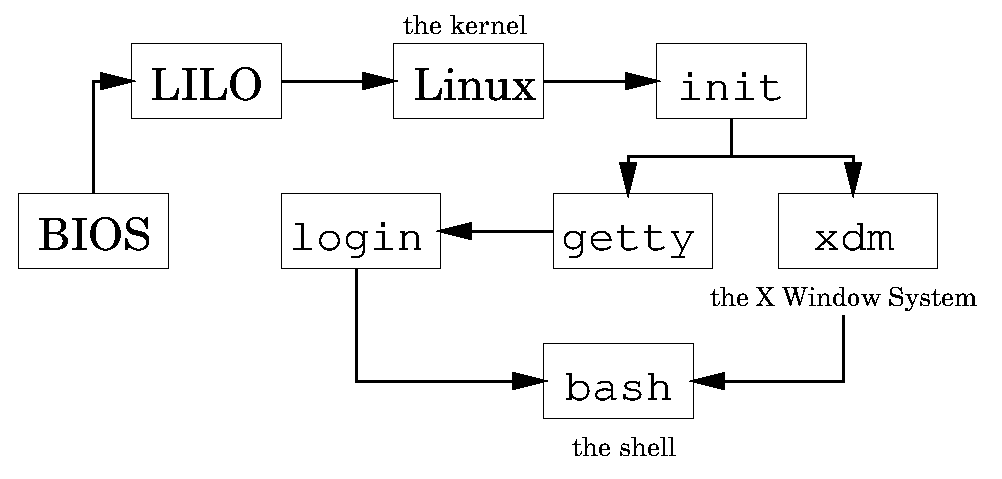
\epsfig{file=ps-files/bootup-figure.ps, width=.9\linewidth}
\caption{The path an Intel PC takes to get to a shell prompt. {\tt
    init} may or may not start the X Window System.  If it does, {\tt
    xdm} runs.  Otherwise, {\tt getty} runs.}
\end{figure}

\linux\ then looks at the type of hardware it's running on.  It wants
to know what type of hard disks you have, whether or not you have a
bus mouse, whether or not you're on a network, and other bits of
trivia like that.  \linux\ can't remember things between boots, so it
has to ask these questions each time it starts up.  Luckily, it isn't
asking {\em you\/} these questions---it is asking the hardware!
During boot-up, the \linux\ kernel will print variations on several
messages. You can read about the messages in
Section~\ref{kernel-messages}.  This query process can some cause
problems with your system but if it was going to, it probably would
have when you first installed \linux.  If you're having problems,
consult your distribution's documentation.

The kernel merely manages other programs, so once it is satisfied
everything is okay, it must start another program to do anything
useful. The program the kernel starts is called {\tt init}
\ttindex{init}.  (Notice the difference in font.  Things in {\tt this
  font} are usually the names of programs, files, directories, or
other computer related items.) After the kernel starts {\tt
  init}\ttindex{init}, it never starts another program. The kernel
becomes a manager and a provider, not an active program.

So to see what the computer is doing after the kernel boots up, we'll
have to examine {\tt init}\ttindex{init}. {\tt init}\ttindex{init}
goes through a complicated startup sequence that isn't the same for
all computers.  \linux\ has many different versions of {\tt
  init}\ttindex{init}, and each does things its own way. It also
matters whether your computer is on a network and what distribution
you used to install \linux. Some things that might happen once {\tt
  init}\ttindex{init} is started:

\begin{itemize}
\item The file systems\glossary{file system} might be checked. What is
  a file system?  A file system is the layout of files on the hard
  disk.  It let's \linux\ know which parts of the disk are already
  used, and which aren't.  (It's like an index to a rather large
  filing system or a card catalog to a library.)  Unfortunately, due
  to various factors such as power losses, what the file system
  information thinks is going on in the rest of the disk and the
  actually layout of the rest of the disk are occasionally in
  conflict. A special program, called {\tt fsck}, can find these
  situations and hopefully correct them.

\item Special routing\glossary{route} programs for
  networks\glossary{network} are run.  These programs tell your
  computer how it's suppose to contact other computers.

\item Temporary files left by some programs may be deleted.

\item The system clock can be correctly updated.  This is trickier
  then one might think, since \unix, by default, wants the time in UCT
  (Universal Coordinated Time, also known as Greenwich Mean Time) and
  your CMOS clock, a battery powered clock in your computer, is
  probably set on local time.  This means that some program must read
  the time from your hardware clock and correct it to UCT.
\end{itemize}

After {\tt init}\ttindex{init} is finished with its duties at boot-up,
it goes on to its regularly scheduled activities. {{\tt init}}
\ttindex{init} can be called the parent of all processes
\index{process}\glossary{process} on a \unix\ system.  A process is
simply a running program.  Since one program can be running two or
more times, there can be two or more processes for any particular
program.

In \unix, a process\index{process}, an instance of a program, is
created by a system call\glossary{system call}---a service provided by
the kernel---called fork\index{process!forking}.  (It's called
``fork'' since one process splits off into two seperate ones.)  {\tt
  init}\ttindex{init} forks a couple of processes, which in turn fork
some of their own. On your \linux\ system, what {\tt init} runs are
several instances of a program called {\tt getty}.\ttindex{getty} {\tt
  getty} is the program that will allow a user to login and eventually
calls a program called {\tt login}\ttindex{login}.

\section{The User Acts}\label{actual-login-section}

\subsection{Logging In}

The first thing you have to do to use a \unix\ machine is to identify
yourself.  The \concept{login} is \unix's way of knowing that users
are authorized to use the system.  It asks for an account
name\index{account} and password.\index{password} An account name is
normally similar to your regular name; you should have already
received one from your system administrator, or created your own if
you are the system administrator. (Information on doing this should be
available in \ldpgs\ or \ldpsa.)

You should see, after all the boot-up procedures are done, something
like the following (the first line is merely a greeting message---it
might be a disclaimer or anything else):

\begin{screen}\begin{verbatim}
Welcome to the mousehouse. Please, have some cheese.

mousehouse login:
\end{verbatim}\end{screen}

\xwarn However, it's possible that what the system presents you
with does {\em not\/} look like this. Instead of a boring text mode
screen, it is graphical. However, it will still ask you to login, and
will function mostly the same way.  If this is the case on your
system, you are going to be using The X Window System\index{X Window
  System}.  This means that you will be presented with a windowing
system.  Chapter~\ref{x-chapter} will discuss some of the differences
that you'll be facing.  Logging in will be similar as will the basics
to much of \unix. If you are using X, look for a giant X is the
margin.

This is, of course, your invitation to login.\index{login} Throughout
this manual, we'll be using the fictional (or not so fictional,
depending on your machine) user {\tt larry}.  Whenever you see {\tt
  larry}, you should be substituting your own account name.  Account
names are usually based on real names; bigger, more serious \unix\ 
systems will have accounts using the user's last name, or some
combination of first and last name, or even some numbers. Possible
accounts for Larry Greenfield might be: {\tt larry}, {\tt greenfie},
{\tt lgreenfi}, {\tt lg19}.

{\tt mousehouse} is, by the way, the ``name'' of the machine I'm
working on. It is possible that when you installed \linux, you were
prompted for some very witty name. It isn't very important, but
whenever it comes up, I'll be using {\tt mousehouse} or, rarely, {\tt
lionsden} when I need to use a second system for clarity or contrast.

After entering {\tt larry} and pressing \ret, I'm faced with the
following:

\begin{screen}\begin{verbatim}
mousehouse login: larry
Password:
\end{verbatim}\end{screen}

What \linux\ is asking for is your \concept{password}. When you type
in your password, you won't be able to see what you type. Type
carefully: it is possible to delete, but you won't be able to see what
you are editing. Don't type too slowly if people are
watching---they'll be able to learn your password.  If you mistype,
you'll be presented with another chance to login.
\glossary{password}\index{password}

If you've typed your login name and password correctly, a short
message will appear, called the message of the day.  
\ttindex{/etc/motd} This could say anything---the system adminstrator
decides what it should be.  After that, a {\bf prompt}
appears.\index{shell!prompt} A prompt is just that, something
prompting you for the next command to give the system. It should look
something like this:

\begin{screen}\begin{verbatim}
/home/larry#
\end{verbatim}\end{screen}

\xwarn If you've already determined you're using X, you'll
probably see a prompt like the one above in a ``window'' somewhere on
the screen. (A ``window'' is a rectangular box.)  To type into
the prompt, move the mouse cursor (it probably looks like a big ``x''
or an arrow) using the mouse into the window.

\subsection{Leaving the Computer}

\cautionpar Do not just turn off the computer! You risk losing
valuable data!

Unlike most versions of DOS\index{DOS}, it's a bad thing to just hit
the power switch when you're done using the computer.  It is also bad
to reboot the machine (with the reset button) without first taking
proper precautions.  \linux, in order to improve performance, has a
\concept{disk cache}.  This means it temporarily stores part of the
computer's permanent storage in RAM\@.\footnote{The difference between
  ``RAM'' and a hard disk is like the difference between short term
  memory and long term memory.  Shutting off the power is like giving
  the computer a knock on the head---it'll forget everything in short
  term memory.  But things saved in long term memory, the hard disk,
  will be okay.  The disk is thousands of times slower than RAM\@.}
The idea of what \linux\ thinks the disk should be and what the disk
actually contains is syncronized every 30 seconds.  In order to turn
off or reboot the computer, you'll have to go through a procedure
telling it to stop caching disk information.

If you're done with the computer, but are logged in (you've entered a
username and password), first you must logout. To do so, enter the
command {\tt logout}. All commands are sent by pressing \ret. Until
you hit return nothing will happen and you can delete what you've
done and start over.

\begin{screen}\begin{verbatim}
/home/larry# logout

Welcome to the mousehouse. Please, have some cheese.

mousehouse login:
\end{verbatim}\end{screen}

Now another user can login.

\subsection{Turning the Computer Off}

If this is a single user system, you might want to turn the computer
off when you're done with it.\footnote{To avoid possibly weakening
  some hardware components, only turn off the computer when you're
  done for the day.  Turning the computer on and off once a day is
  probably the best compromise between energy and wear \& tear on the
  system.} To do so, you'll have to log into a special account called
{\tt root}. The {\tt root} account is the system adminstrator's
account and can access any file on the system.  If you're going to
turn the computer off, get the password from the system adminstrator.
(In a single user system, that's {\em you\/}!  Make sure you know the
{\tt root} password.) Login as {\tt root}:

\begin{screen}\begin{verbatim}
mousehouse login: root
Password:
Linux version 1.3.55 (root@mousehouse) #1 Sun Jan 7 14:56:26 EST 1996
/# shutdown now
Why? end of the day

URGENT: message from the sysadmin:
System going down NOW

          ... end of the day ...

Now you can turn off the power...
\end{verbatim}\end{screen}

The command {\tt shutdown now} prepares the system to be reset or
turned off.  Wait for a message saying it is safe to and then reset or
turn off the system.  (When the system asks you
``Why?'', it is merely asking for a reason to tell other users.  Since
no one is using the system when you shut it down, you can tell it
anything you want or nothing at all.)

A quick message to the lazy: an alternative to the logout/login
approach is to use the command {\tt su}. As a normal user, from your
prompt, type {\tt su} and press \ret. It should prompt you for the
root password, and then give you root privileges. Now you can shutdown
the system with the {\tt shutdown now} command.

\section{Kernel Messages}\label{kernel-messages}

When you first start your computer, a series of messages flash across
the screen describing the hardware that is attached to your
computer.  These messages are printed by the \linux\ kernel.  In this
section, I'll attempt to describe and explain those messages.

Naturally, these messages differ from machine to machine.  I'll
describe the messages I get for my machine.  The following example
contains all of the standard messages and some specific ones.  (In
general, the machine I'm taking this from is a minimally configured
one: you won't see a lot of device specific configuration.)  This was
made with Linux version 1.3.55---one of the most recent as of this
writing.

\index{linux kernel!starting messages@\linux\ kernel!starting messages}
\begin{enumerate}
\item The first thing \linux\ does is decides what type of video card
and screen you have, so it can pick a good font size. (The smaller the
font, the more that can fit on the screen on any one time.) \linux\
may ask you if you want a special font, or it might have had a choice
compiled in.\footnote{``Compiled'' is the process by which a computer
program that a human writes gets translated into something the
computer understands.  A feature that has been ``compiled in'' has
been included in the program.}
\begin{screen}\begin{verbatim}
Console: 16 point font, 400 scans
Console: colour VGA+ 80x25, 1 virtual console (max 63)
\end{verbatim}\end{screen}
In this example, the machine owner decided he wanted the standard,
large font at compile time.\glossary{compile}\glossary{binary} Also,
note the misspelling of the word ``color.'' Linus evidently learned
the wrong version of English.\index{Torvalds, Linus!English usage}

\item The next thing the kernel will report is how fast your system
  is, as measured by ``BogoMIPS''.\index{BogoMIPS}  A ``MIP'' stands
  for a million instructions per second, and a ``BogoMIP'' is a
  ``bogus MIP'': how many times the computer can do absolutely nothing
  in one second.  (Since this loop doesn't actually do anything, the
  number is not actually a measure of how fast the system is.)
  \linux\ uses this number when it needs to wait for a hardware
  device.
\begin{screen}\begin{verbatim}
Calibrating delay loop.. ok - 33.28 BogoMIPS
\end{verbatim}\end{screen}
  
\item The \linux\ kernel also tells you a little about memory usage:
  \begin{screen}\begin{verbatim}
Memory: 23180k/24576k available (544k kernel code, 384k reserved, 468k data)
\end{verbatim}\end{screen}
This said that the machine had 24 megabytes\glossary{megabyte} of
memory.  Some of this memory was reserved for the kernel.  The rest of
it can be used by programs.  This is the temporary \concept{RAM} that
is used only for short term storage.  Your computer also has a
permanent memory called a \concept{hard disk}.  The hard disk's
contents stay around even when power is turned off.

\item Throughout the bootup procedure, \linux\ tests different parts
  of the hardware and prints messages about these tests.
\begin{screen}\begin{verbatim}
This processor honours the WP bit even when in supervisor mode. Good.
\end{verbatim}\end{screen}

  \item Now \linux\ moves onto the network
    configuration.\glossary{network} The following should be described
    in \ldpng, and is beyond the scope of this document.
\begin{screen}\begin{verbatim}
Swansea University Computer Society NET3.033 for Linux 1.3.50
IP Protocols: ICMP, UDP, TCP
\end{verbatim}\end{screen}

  \item \linux\ supports a FPU\index{FPU}, a floating point unit. This
    is a special chip (or part of a chip, in the case of a 80486DX
    CPU\glossary{floating point unit}) that performs arithmetic
    dealing with non-whole numbers. Some of these chips are bad, and
    when \linux\ tries to identify these chips, the machine
    ``crashes''.  The machine stops functioning. If this happens,
    you'll see:
\begin{screen}\begin{verbatim}
Checking 386/387 coupling...
\end{verbatim}\end{screen}\index{error!bad 386/387 coupling}
Otherwise, you'll see:
\begin{screen}\begin{verbatim}
Checking 386/387 coupling... Ok, fpu using exception 16 error reporting.
\end{verbatim}\end{screen}
if you're using a 486DX\@.  If you are using a 386 with a 387, you'll see:
\begin{screen}\begin{verbatim}
Checking 386/387 coupling... Ok, fpu using irq13 error reporting.
\end{verbatim}\end{screen}

\item It now runs another test on the ``halt'' instruction.
\begin{screen}\begin{verbatim}
Checking 'hlt' instruction... Ok.
\end{verbatim}\end{screen}
  
\item After that initial configuration, \linux\ prints a line
  identifying itself.  It says what version it is, what
  version of the GNU C Compiler compiled it, and when it was compiled.
\begin{screen}\begin{verbatim}
Linux version 1.3.55 (root@mousehouse) (gcc version 2.7.0) #1 Sun Jan 7 14:56:26 EST 1996
\end{verbatim}\end{screen}

  \item The serial \index{serial ports} driver has started to ask
    questions about the hardware.  A \concept{driver} is a part of the
    kernel that controls a device, usually a peripheral.  It is
    responsible for the details of how the CPU communicates with the
    device.  This allows people who write user applications to
    concentrate on the application: they don't have to worry about
    exactly how the computer works.
\begin{screen}\begin{verbatim}
Serial driver version 4.11 with no serial options enabled
tty00 at 0x03f8 (irq = 4) is a 16450
tty01 at 0x02f8 (irq = 3) is a 16450
tty02 at 0x03e8 (irq = 4) is a 16450
\end{verbatim}\end{screen}
Here, it found 3 serial ports.  A serial port is the equivalent of
a DOS\index{DOS} {\tt COM} port, and is a device normally used to
communicate with
modems and mice.

What it is trying to say is that serial port 0 ({\tt COM1}) has an
address of {\tt 0x03f8}. When it interrupts the kernel,
usually to say that it has data, it uses IRQ 4. An IRQ is another
means of a peripheral talking to the software.  Each serial port also
has a controller chip.  The usual one for a port to have is a 16450;
other values possible are 8250 and 16550. 

\item Next comes the parallel port driver.  A parallel port is
\index{parallel ports}
normally connected to a printer, and the names for the parallel ports
(in \linux) start with {\tt lp}. {\tt lp} stands for {\bf L}ine {\bf
P}rinter, although in modern times it makes more sense for it to stand
for {\bf L}aser {\bf P}rinter.  (However, \linux\ will happily
communicate with any sort of parallel printer: dot matrix, ink jet, or
laser.)
\begin{screen}\begin{verbatim}
lp0 at 0x03bc, (polling)
\end{verbatim}\end{screen}
That message says it has found one parallel port, and is using the
standard driver for it.

\item \linux\ next identifies your hard disk drives.  In the example
  system I'm showing you, {\tt mousehouse}, I've installed two IDE
  hard disk drives.
\begin{screen}\begin{verbatim}
hda: WDC AC2340, 325MB w/127KB Cache, CHS=1010/12/55
hdb: WDC AC2850F, 814MB w/64KB Cache, LBA, CHS=827/32/63
\end{verbatim}\end{screen}
  

\item The kernel now moves onto looking at your floppy drives. In this
example, the machine has two drives: drive ``A'' is
a $5\ {1/4}$ inch drive, and drive ``B'' is a $3\ {1/2}$ inch drive.
\linux\ calls drive ``A'' {\tt fd0} and drive ``B'' {\tt fd1}.
\begin{screen}\begin{verbatim}
Floppy drive(s): fd0 is 1.44M, fd1 is 1.2M
floppy: FDC 0 is a National Semiconductor PC87306
\end{verbatim}\end{screen}

\item The next driver to start on my example system is the SLIP
  driver.  It prints out a message about its configuration.
\begin{screen}\begin{verbatim}
SLIP: version 0.8.3-NET3.019-NEWTTY (dynamic channels, max=256) (6 bit encapsulation enabled)
CSLIP: code copyright 1989 Regents of the University of California
\end{verbatim}\end{screen}

  \item The kernel also scans the hard disks it found.  It will look
    for the different partitions on each of them.  A partition is a
    logical separation on a drive that is used to keep operating
    systems from interfering with each other. In this example, the
    computer had two hard disks ({\tt hda}, {\tt hdb}) with four
    partitions and one partition, respectively.\index{partition!disk}
\begin{screen}\begin{verbatim}
Partition check:
  hda: hda1 hda2 hda3 hda4
  hdb: hdb1
\end{verbatim}\end{screen}

\item Finally, \linux\ {\bf mounts}\glossary{mount}\index{mount} the
  root partition.  The root partition is the disk partition where the
  \linux\ operating system resides.\index{partition!root}  When
  \linux\ ``mounts'' this partition, it is making the partition
  available for use by the user.
\begin{screen}\begin{verbatim}
VFS: Mounted root (ext2 filesystem) readonly.
\end{verbatim}\end{screen}
\end{enumerate} % kernel start-up messages
% Local Variables: 
% mode: latex
% TeX-master: "guide"
% End: 


% introduction to the shell: commands, storing information
\chapter{The \unix\ Shell}\label{shell-chapter}

\begin{fortune}
\raggedright
Making files is easy under the UNIX operating system.  Therefore,
users tend to create numerous files using large amounts of file
space.  It has been said that the only standard thing about all UNIX
systems is the message-of-the-day telling users to clean up their
files.\\
\raggedleft System V.2 administrator's guide
\end{fortune}

\section{\unix\ Commands}

When you first log into a \unix\ system, you are presented with
something that looks like the following:

\begin{screen}
\begin{verbatim}
/home/larry#
\end{verbatim}
\end{screen}

That ``something'' is called a \concept{prompt}.  As its name would
suggest, it is prompting you to enter a command.  Every \unix\ command
is a sequence of letters, numbers, and characters.\glossary{character}
There are no spaces, however.  Some valid \unix\ commands are {\tt
  mail}, {\tt cat}, and {\tt CMU\_is\_Number-5}.  Some characters
aren't allowed---we'll go into that later.  \unix\ is also
\concept{case-sensitive}.  This means that {\tt cat} and {\tt Cat} are
different commands.\footnote{Case sensitivity is a very personal
  thing.  Some operating systems, such as OS/2\index{OS/2} or Windows
  NT\index{Windows NT} are case preserving, but not case sensitive.
  In practice, \unix\ rarely uses the different cases.  It is unusual
  to have a situation where {\tt cat} and {\tt Cat} are different
  commands.}

The prompt is displayed by a special program called the
\concept{shell}.  Shells accept commands, and run those commands. They
can also be programmed in their own language, and programs written in
that language are called ``shell
scripts''.\index{shell!programming}\index{shell!script}

There are two major types of shells in \unix: Bourne shells and C
shells.  Bourne shells are named after their inventor, Steven
Bourne.\index{Bourne, Steve R.} Steven Bourne wrote the original
\unix\ shell {\tt sh}\ttindex{sh}, and most shells since then end in
the letters {\tt sh} to indicate they are extentions on the original
idea.  There are many implementations of his shell, and all those
specific shell programs are called Bourne shells. Another class of
shells, C shells (originally implemented by Bill Joy\index{Joy,
  Bill}), are also common. Traditionally, Bourne shells have been used
for shell scripts and compatibility with the original {\tt sh} while C
shells have been used for interactive use.  (C shells have had the
advantages of having better interactive features but somewhat harder
programming features.)

\linux\ comes with a Bourne shell called {\tt bash}\ttindex{bash},
written by the Free Software Foundation.\index{Free Software Foundation} 
{\tt bash} stands for {\bf B}ourne {\bf A}gain {\bf Sh}ell, one of the
many bad puns in \unix.  It is an ``advanced'' Bourne shell:  it
contains the standard programming features found in all Bourne shells
with many interactive features commonly found in C shells.  {\tt bash}
is the default shell to use running \linux.

When you first login, the prompt is displayed by {\tt bash}, and you
are running your first \unix\ program, the {\tt bash} shell.  As long
as you are logged in, the {\tt bash} shell will constantly be running.

\subsection{A Typical \unix\ Command}

The first command to know is {\tt cat}\ttindex{cat}.  To use it,
type {\tt cat}, and then \ret:

\begin{screen}\begin{verbatim}
/home/larry# cat

\end{verbatim}\end{screen}

If you now have a cursor on a line by itself, you've done the correct
thing.  There are several variances you could have typed---some would
work, some wouldn't.

\begin{itemize}
\item If you misspelled {\tt cat}, you would have seen
\begin{screen}\begin{verbatim}
/home/larry# ct
ct: command not found
/home/larry#
\end{verbatim}\end{screen}
Thus, the shell informs you that it couldn't find a program named
``{\tt ct}'' and gives you another prompt to work with. Remember,
\unix\ is case sensitive: {\tt CAT} is a misspelling.
\item You could have also placed whitespace before the command, like
  this:\footnote{The `{\tt \char `\ }' indicates that the user typed a
    space.}
\begin{screen}\begin{verbatim*}
/home/larry#     cat     
\end{verbatim*}\end{screen}
This produces the correct result and runs the {\tt cat} program.
% any more ideas for common things?
\item You might also press return on a line by itself. Go right
  ahead---it does absolutely nothing.
\end{itemize}

I assume you are now in {\tt cat}\ttindex{cat}.  Hopefully, you're
wondering what it is doing.  No, it is not a game.  {\tt cat} is a
useful utility that won't seem useful at first.  Type anything and
hit return.  What you should have seen is:

\begin{tscreen}
/home/larry\# cat\\
{\sl Help! I'm stuck in a Linux program!}\\
Help! I'm stuck in a Linux program!
\end{tscreen}

(The {\sl slanted\/} text indicates what I typed to {\tt cat}.) What
{\tt cat} seems to do is echo the text right back at yourself.  This
is useful at times, but isn't right now.  So let's get out of this
program and move onto commands that have more obvious benefits.

To end many \unix\ commands, type \eof\footnote{Hold down the key
  labeled ``Ctrl'' and press ``d'', then let go of both.}. \eof\ is
the end-of-file character, or EOF for short.\index{end-of-text}
\index{end-of-file} Alternatively, it stands for end-of-text,
depending on what book you read.  I'll refer to it as an end-of-file.
It is a control character that tells \unix\ programs that you (or
another program) is done entering data.  When {\tt cat} sees you
aren't typing anything else, it terminates.

For a similar idea, try the program {\tt sort}.\ttindex{sort} As its
name indicates, it is a sorting program.  If you type a couple of
lines, then press \eof, it will output those lines in a sorted order.
These types of programs are called {\bf filters}\glossary{filter},
because they take in text, filter it, and output the text slightly
differently.  Both {\tt cat} and {\tt sort} are unusual filters.  {\tt
  cat} is unusual because it reads in text and performs \emph{no}
changes on it.  {\tt sort} is unusual because it reads in lines and
doesn't output anything until after it's seen the EOF character.  Many
filters run on a line-by-line basis: they will read in a line, perform
some computations, and output a different line.

\section{Helping Yourself}\label{man-section}\bindex{help!on-line}

The {\tt man}\impttindex{man} command displays reference pages for the
command\footnote{{\tt man} will also display information on a system
  call, a subroutine, a file format, and more.  In the original
  version of \unix\ it showed the exact same information the printed
  documentation would.  For now, you're probably only interested in
  getting help on commands.} you specify. For example:

\begin{screen}
\begin{verbatim}
/home/larry# man cat

cat(1)                                                     cat(1)

NAME
  cat - Concatenates or displays files

SYNOPSIS
  cat [-benstuvAET] [--number] [--number-nonblank] [--squeeze-blank]
  [--show-nonprinting] [--show-ends] [--show-tabs] [--show-all]
  [--help] [--version] [file...]

DESCRIPTION
  This manual page documents the GNU version of cat ...
\end{verbatim}
\end{screen}

There's about one full page of information about {\tt cat}. Try
running {\tt man} now.  Don't expect to understand the manpage given.
Manpages usually assume quite a bit of \unix\ knowledge---knowledge
that you might not have yet.  When you've read the page, there's
probably a little black block at the bottom of your screen similar to
``{\tt --more--}'' or ``{\tt Line 1}''.  This is the
\concept{more-prompt}, and you'll learn to love it.

Instead of just letting the text scroll away, {\tt man} stops at the
end of each page, waiting for you to decide what to do now. If you
just want to go on, press \key{Space}\ and you'll advance a page. If
you want to exit (quit) the manual page you are reading, just press
\key{q}. You'll be back at the shell prompt, and it'll be waiting for
you to enter a new command.

There's also a keyword function in {\tt man}. For example, say you're
interested in any commands that deal with Postscript, the printer
control language from Adobe. Type {\tt man -k ps} or {\tt man -k
  Postscript}, you'll get a listing of all commands, system calls, and
other documented parts of \unix\ that have the word ``ps'' (or
``Postscript'') in their name or short description. This can be very
useful when you're looking for a tool to do something, but you don't
know it's name---or if it even exists!

\eindex{help!on-line}

\section{Storing Information}

Filters are very useful once you are an experienced user, but they
have one small problem.  How do you store the information?  Surely you
aren't expected to type everything in each time you are going to use
the program! Of course not. \unix\ provides {\bf files} and {\bf
  directories}.\glossary{directory}

A directory is like a folder: it contains pieces of paper, or files.
A large folder can even hold other folders---directories can be inside
directories.  In \unix, the collection of directories and files is
called the file system.\index{file system} Initially, the file system
consists of one directory, called the ``root''
directory.\index{directory!root} Inside this directory, there are more
directories, and inside those directories are files and yet more
directories.\footnote{There may or may not be a limit to how ``deep''
  the file system can go.  (I've never reached it---one can easily
  have directories 10 levels deep.)}

Each file and each directory has a name.  It has both a short name, which
can be the same as another file or directory somewhere else on the system,
and a long name which is unique.  A short name for a file could be {\tt
joe}, while it's ``full name'' would be {\tt /home/larry/joe}. The full
name is usually called the {\bf path}\glossary{path}.  The path can be
decode into a sequence of directories.  For example, here is how {\tt
/home/larry/joe} is read:
\begin{tabbing}
\tt /\=\tt home/\=\tt larry/\=\tt joe\\
The initial slash indicates the root directory.\+\\
This signifies the directory called {\tt home}. It is inside the
root directory.\+\\
This is the directory {\tt larry}, which is inside {\tt home}.\+\\
{\tt joe} is inside {\tt larry}.  A path could refer to either a
directory or a filename,\\ so {\tt joe} could be either.  All the items
{\em before\/} the short name must be directories.
\end{tabbing}

An easy way of visualizing this is a tree diagram.  To see a diagram
of a typical \linux\ system, look at Figure~\ref{standard-dirtree}.
Please note that this diagram isn't complete---a full \linux\ system
has over 8000 files!---and shows only some of the standard
directories.  Thus, there may be some directories in that diagram that
aren't on your system, and your system almost certainly has
directories not listed there.

\unitlength=1.0pt
\begin{figure}[bt]
\caption{A typical (abridged) Unix directory tree.}
\label{standard-dirtree}
\begin{picture}(148.00,365.00)(0.00,450.00)
\put(9.00,805.00){\line(1,0){29.00}} % / -> bin
\put(26.00,805.00){\line(0,-1){112.00}} % /'s children
\put(26.00,791.00){\line(1,0){12.00}} % dev
\put(26.00,777.00){\line(1,0){12.00}} % etc
\put(26.00,763.00){\line(1,0){12.00}} % home
\put(64.50,763.00){\line(1,0){29.00}} % home -> larry
\put(81.50,763.00){\line(0,-1){14.00}} % home's children
\put(81.50,749.00){\line(1,0){12.00}} % sam
\put(26.00,735.00){\line(1,0){12.00}} % lib
\put(26.00,721.00){\line(1,0){12.00}} % proc
\put(26.00,707.00){\line(1,0){12.00}} % tmp
\put(26.00,693.00){\line(1,0){12.00}} % usr
\put(55.50,693.00){\line(1,0){29.00}} % usr -> X386
\put(72.50,693.00){\line(0,-1){238.00}} % usr's children
\put(72.50,676.00){\line(1,0){12.00}} % bin
\put(72.50,659.00){\line(1,0){12.00}} % emacs
\put(72.50,642.00){\line(1,0){12.00}} % etc
\put(72.50,625.00){\line(1,0){12.00}} % g++-include
\put(72.50,608.00){\line(1,0){12.00}} % include
\put(72.50,591.00){\line(1,0){12.00}} % lib
\put(72.50,574.00){\line(1,0){12.00}} % local
\put(107.00,574.00){\line(1,0){29.00}} % local -> bin
\put(124.00,574.00){\line(0,-1){51.00}} % local's children
\put(124.00,557.00){\line(1,0){12.00}} % emacs
\put(124.00,540.00){\line(1,0){12.00}} % etc
\put(124.00,523.00){\line(1,0){12.00}} % lib
\put(72.50,506.00){\line(1,0){12.00}} % man
\put(72.50,489.00){\line(1,0){12.00}} % spool
\put(72.50,472.00){\line(1,0){12.00}} % src
\put(100.50,472.00){\line(1,0){29.00}} % src -> linux
\put(72.50,455.00){\line(1,0){12.00}} % tmp
\put(8.50,805.00){\makebox(0,0)[rc]{/}}
\put(39.50,805.00){\makebox(0,0)[lc]{bin}}
\put(39.50,791.00){\makebox(0,0)[lc]{dev}}
\put(39.50,777.00){\makebox(0,0)[lc]{etc}}
\put(39.50,763.00){\makebox(0,0)[lc]{home}}
\put(95.00,763.00){\makebox(0,0)[lc]{larry}}
\put(95.00,749.00){\makebox(0,0)[lc]{sam}}
\put(39.50,735.00){\makebox(0,0)[lc]{lib}}
\put(39.50,721.00){\makebox(0,0)[lc]{proc}}
\put(39.50,707.00){\makebox(0,0)[lc]{tmp}}
\put(39.50,693.00){\makebox(0,0)[lc]{usr}}      % I'm expecting you to
\put(86.00,693.00){\makebox(0,0)[lc]{X11R6}}    % proof-read this!
\put(86.00,676.00){\makebox(0,0)[lc]{bin}}      
\put(86.00,659.00){\makebox(0,0)[lc]{emacs}}    % I am, I am, don't worry! :-)
\put(86.00,642.00){\makebox(0,0)[lc]{etc}}
\put(86.00,625.00){\makebox(0,0)[lc]{g++-include}}
\put(86.00,608.00){\makebox(0,0)[lc]{include}}
\put(86.00,591.00){\makebox(0,0)[lc]{lib}}
\put(86.00,574.00){\makebox(0,0)[lc]{local}}
\put(137.50,574.00){\makebox(0,0)[lc]{bin}}
\put(137.50,557.00){\makebox(0,0)[lc]{emacs}}
\put(137.50,540.00){\makebox(0,0)[lc]{etc}}
\put(137.50,523.00){\makebox(0,0)[lc]{lib}}
\put(86.00,506.00){\makebox(0,0)[lc]{man}}
\put(86.00,489.00){\makebox(0,0)[lc]{spool}}
\put(86.00,472.00){\makebox(0,0)[lc]{src}}
\put(130.50,472.00){\makebox(0,0)[lc]{linux}}
\put(86.00,455.00){\makebox(0,0)[lc]{tmp}}
\end{picture}
\end{figure}

\subsection{Looking at Directories with {\tt ls}}

Now that you know that files and directories exist, there must be some
way of manipulating them.  Indeed there is.  The command {\tt
  ls}\ttindex{ls} is one of the more important ones. It {\bf l}i{\bf
  s}ts files.  If you try {\tt ls} as a command, you'll see:

\begin{screen}\begin{verbatim}
/home/larry# ls
/home/larry#
\end{verbatim}\end{screen}

That's right, you'll see nothing. \unix\ is intensionally terse: it
gives you nothing, not even ``no files'' if there aren't any files.
Thus, the lack of output was {\tt ls}'s way of saying it didn't find
any files.

But I just said there could be 8000 or more files lying around: where
are they? You've run into the concept of a ``current'' directory. You
can see in your prompt that your current directory is {\tt
  /home/larry}, where you don't have any files.  If you want a list of
files of a more active directory, try the root directory:

\begin{screen}\begin{verbatim}
/home/larry# ls /
bin      etc      install  mnt      root     user     var
dev      home     lib      proc     tmp      usr      vmlinux
/home/larry# 
\end{verbatim}
\end{screen}

In the above command, ``{\tt ls /}'', the directory (``{\tt /}'') is a
\concept{parameter}. The first word of the command is the command
name, and anything after it is a parameter.  Parameters generally
modify what the program is acting on---for {\tt ls}, the parameters
say what directory you want a list for.  Some commands have special
parameters called options or switches. To see this try:

\begin{screen}\begin{verbatim}
/home/larry# ls -F /
bin/      etc/      install/  mnt/      root/     user/     var@
dev/      home/     lib/      proc/     tmp/      usr/      vmlinux
/home/larry# 
\end{verbatim}
\end{screen}

The {\tt -F} is an \concept{option}.  An option is a special kind of
parameter that starts with a dash and modifies how the program runs,
but not what the program runs on.  For {\tt ls}, {\tt -F} is an option
that lets you see which ones are directories, which ones are special
files, which are programs, and which are normal files.  Anything with
a slash is a directory. We'll talk more about {\tt ls}'s features
later. It's a surprisingly complex program!

Now, there are two lessons to be learned here. First, you should learn
what {\tt ls} does. Try a few other directories that are shown in
Figure~\ref{standard-dirtree}, and see what they contain. Naturally,
some will be empty, and some will have many, many files in them.  I
suggest you try {\tt ls} both with and without the {\tt -F} option.
For example, {\tt ls /usr/local} looks like:

\begin{screen}\begin{verbatim}
/home/larry# ls /usr/local
archives  bin       emacs     etc       ka9q      lib       tcl
/home/larry# 
\end{verbatim}
\end{screen}

The second lesson is more general. Many \unix\ commands are like {\tt
  ls}. They have options, which are generally one character after a
dash, and they have parameters.  Unlike {\tt ls}, some commands
\emph{require} certain parameters and/or options.  To show what
commands generally look like, we'll use the following form:

\begin{command}
{\tt ls} [-aRF] [{\sl directory}]
\end{command}

I'll generally use command templates like that before I introduce any
command from now on.  The first word is the command (in this case {\tt
  ls}).  Following the command are all the parameters.  Optional
parameters are contained in brackets (``['' and ``]'').
Meta-variables are {\sl slanted\/}---they're words that take the place
of actual parameters.  (For example, above you see {\sl directory},
which should be replaced by the name of a real directory.)

Options are a special case.  They're enclosed by brackets, but you can
take any one of them without using all of them.  For instance, with
just the three options given for {\tt ls} you have eight different
ways of running the command: with or without each of the options.
(Contrast {\tt ls -R} with {\tt ls -F}.)

\subsection{The Current Directory and {\tt cd}}

\begin{command}
{\tt pwd}
\end{command}

Using directories would be cumbersome if you had to type the full path
each time you wanted to access a directory.  Instead, \unix\ shells
have a feature called the ``current'' or ``present'' or ``working''
directory.  Your setup most likely displays your directory in your
prompt: {\tt /home/larry}. If it doesn't, try the command {\tt pwd},
for {\bf p}resent {\bf w}orking {\bf d}irectory.  (Sometimes the
prompt will display the machine name.  This is only really useful in a
networked environment with lots of different machines.)
\ttindex{pwd}
\index{directory!current}
\index{directory!present}
\index{directory!working}

\begin{screen}\begin{verbatim}
mousehouse>pwd
/home/larry
mousehouse>  
\end{verbatim}
\end{screen}

\begin{command}
{\tt cd} [{\sl directory}]
\end{command}

As you can see, {\tt pwd} tells you your current
directory\footnote{You'll see all the terms in this book: present
  working directory, current directory, or working directory.  I
  prefer ``current directory'', although at times the other forms will
  be used for stylistic purposes.}---a very simple command.  Most
commands act, by default, on the current directory.  For instance,
{\tt ls} without any parameters displays the contents of the current
directory.  We can change our current directory using {\tt
  cd}\ttindex{cd}. For instance, try:

\begin{screen}\begin{verbatim}
/home/larry# cd /home
/home# ls -F
larry/     sam/       shutdown/  steve/     user1/
/home# 
\end{verbatim}
\end{screen}

If you omit the optional parameter {\sl directory}, you're returned to
your home, or original, directory.  Otherwise, {\tt cd} will change
you to the specified directory. For instance:

\begin{screen}\begin{verbatim}
/home# cd
/home/larry# cd /
/# cd home
/home# cd /usr
/usr# cd local/bin
/usr/local/bin#
\end{verbatim}
\end{screen}

As you can see, {\tt cd} allows you to give either absolute or
relative pathnames.  An \concept{absolute path} starts with {\tt /}
and specifies all the directories before the one you wanted.  A
\concept{relative path} is in relation to your current directory.  In
the above example, when I was in {\tt /usr}, I made a relative move to
{\tt local/bin}---{\tt local} is a directory under {\tt usr}, and {\tt
  bin} is a directory under {\tt local}!  ({\tt cd home} was also a
relative directory change.)

There are two directories used {\em only\/} for relative pathnames:
``{\tt .}'' and ``{\tt ..}''.\index{directory!current}
\index{directory!parent}.  The directory ``{\tt .}'' refers
to the current directory and ``{\tt ..}'' is the parent directory.
These are ``shortcut'' directories.  They exist in {\em every\/}
directory, but don't really fit the ``folder in a folder'' concept.
Even the root directory has a parent directory---it's its own parent!

The file {\tt ./chapter-1} would be the file called {\tt chapter-1}
in the current directory.  Occasionally, you need to put the ``{\tt
  ./}'' for some commands to work, although this is rare.  In most
cases, {\tt ./chapter-1} and {\tt chapter-1} will be identical.

The directory ``{\tt ..}'' is most useful in ``backing up'':

\begin{screen}\begin{verbatim}
/usr/local/bin# cd ..
/usr/local# ls -F
archives/  bin/       emacs@     etc/       ka9q/      lib/       tcl@
/usr/local# ls -F ../src
cweb/      linux/     xmris/
/usr/local#
\end{verbatim}\end{screen}

In this example, I changed to the parent directory using {\tt cd ..},
and I listed the directory {\tt /usr/src} from {\tt /usr/local} using
{\tt ../src}. Note that if I was in {\tt /home/larry}, typing {\tt ls
  -F ../src} wouldn't do me any good!

The directory {\tt \verb+~+/} is an alias for your home
directory\index{directory!home}:

\begin{screen}\begin{verbatim}
/usr/local# ls -F ~/
/usr/local# 
\end{verbatim}\end{screen}

You can see at a glance that there isn't anything in your home
directory!  {\tt \verb+~+/} will become more useful as we learn more
about how to manipulate files.

\subsection{Creating and Removing Directories}

\index{mkdir@{\tt mkdir}|(}\bindex{directory!creating} 

\begin{command}
{\tt mkdir} {\sl directory1} [{\sl directory2 \ldots directoryN}]
\end{command}

Creating your own directories is extremely simple under \unix, and can
be a useful organizational tool. To create a new directory, use the
command {\tt mkdir}.  Of course, {\tt mkdir} stands for {\bf m}a{\bf
  k}e {\bf dir}ectory.

Let's do a small example to see how this works:
\begin{screen}\begin{verbatim}
/home/larry# ls -F
/home/larry# mkdir report-1993
/home/larry# ls -F
report-1993/
/home/larry# cd report-1993
/home/larry/report-1993#
\end{verbatim}
\end{screen}

{\tt mkdir} can take more than one parameter, interpreting each
parameter as another directory to create.  You can specify either the
full pathname or a relative pathname; {\tt report-1993} in the above
example is a relative pathname.

\begin{screen}\begin{verbatim}
/home/larry/report-1993# mkdir /home/larry/report-1993/chap1 ~/report-1993/chap2
/home/larry/report-1993# ls -F
chap1/  chap2/
/home/larry/report-1993#
\end{verbatim}\end{screen}

\begin{command}
  {\tt rmdir} {\sl directory1} [{\sl directory2 \ldots directoryN}]
\end{command}

The opposite of {\tt mkdir} is {\tt rmdir} ({\bf r}e{\bf m}ove {\bf
  dir}ectory).  {\tt rmdir} works exactly like {\tt mkdir}.
\ttindex{rmdir}

An example of {\tt rmdir} is:

\begin{screen}\begin{verbatim}
/home/larry/report-1993# rmdir chap1 chap3
rmdir: chap3: No such file or directory
/home/larry/report-1993# ls -F
chap2/
/home/larry/report-1993# cd ..
/home/larry# rmdir report-1993
rmdir: report-1993: Directory not empty
/home/larry#
\end{verbatim}\end{screen}

As you can see, {\tt rmdir} will refuse to remove a non-existant
directory, as well as a directory that has anything in it. (Remember,
{\tt report-1993} has a subdirectory, {\tt chap2}, in it!) There is
one more interesting thing to think about {\tt rmdir}: what happens if
you try to remove your current directory? Let's find out:

\begin{screen}\begin{verbatim}
/home/larry# cd report-1993
/home/larry/report-1993# ls -F
chap2/
/home/larry/report-1993# rmdir chap2
/home/larry/report-1993# rmdir .
rmdir: .: Operation not permitted
/home/larry/report-1993#
\end{verbatim}\end{screen}

Another situation you might want to consider is what happens if you try
to remove the parent of your current directory. This turns out not to
be a problem since the parent of your current directory isn't empty, so
it can't be removed!
\index{mkdir@{\tt mkdir}|)}\eindex{directory!creating}

\section{Moving Information}

All of these fancy directories are very nice, but they really don't
help unless you have some place to store you data.  The \unix\ 
Gods\index{Gods!\unix} saw this problem, and they fixed it by giving
the users \concept{files}.



We will learn more about creating and editing files in the next few
chapters.

The primary commands for manipulating files under \unix\ are {\tt cp},
{\tt mv}, and {\tt rm}.  They stand for {\bf c}o{\bf p}y, {\bf m}o{\bf
  v}e, and {\bf r}e{\bf m}ove, respectively.

\subsection{{\tt cp} Like a Monk}\bttindex{cp}

\begin{command}
{\tt cp} [-i] {\sl source} {\sl destination}\\
{\tt cp} [-i] {\sl file1 file2 \ldots fileN} {\sl
  destination-directory}\footnote{{\tt cp} has two lines in its
  template because the meaning of the second parameter can be
  different depending on the number of parameters.}
\end{command}

{\tt cp} is a very useful utility under \unix, and extremely powerful.  It
enables one person to copy more information in a second than a fourteenth
century monk could do in a year.

\cautionpar Be careful with {\tt cp} if you don't have a lot of disk
space.  No one wants to see a ``Disk full'' message when working on
important files. {\tt cp} can also overwrite existing files without
warning---I'll talk more about that danger later.

We'll first talk about the first line in the command template.  The
first parameter to {\tt cp} is the file to copy---the second is where to
copy it.  You can copy to either a different filename, or a different
directory. Let's try some examples:

\begin{screen}\begin{verbatim}
/home/larry# ls -F /etc/passwd
/etc/passwd
/home/larry# cp /etc/passwd .
/home/larry# ls -F
passwd
/home/larry# cp passwd frog
/home/larry# ls -F
frog  passwd
/home/larry#
\end{verbatim}
\end{screen}

The first {\tt cp} command I ran took the file {\tt
  /etc/passwd}\ttindex{/etc/passwd}, which contains the names of all
the users on the \unix\ system and their (encrypted) passwords, and
copied it to my home directory.  {\tt cp} doesn't delete the source
file, so I didn't do anything that could harm the system.  So two
copies of {\tt /etc/passwd} exist on my system now, both named {\tt
  passwd}, but one is in the directory {\tt /etc} and one is in {\tt
  /home/larry}.

Then I created a {\em third\/} copy of {\tt
  /etc/passwd}\ttindex{/etc/passwd} when I typed {\tt cp passwd
  frog}---the three copies are now: {\tt /etc/passwd}, {\tt
  /home/larry/passwd} and {\tt /home/larry/frog}. The contents of
these three files are the same, even if the names aren't.

{\tt cp} can copy files between directories if the first parameter is a
file and the second parameter is a directory.  In this case, the short
name of the file stays the same.

It can copy a file and change it's name if both parameters are file
names. Here is one danger of {\tt cp}. If I typed {\tt cp /etc/passwd
/etc/group}, {\tt cp} would normally create a new file with the contents
identical to {\tt passwd} and name it {\tt group}.  However, if {\tt
/etc/group} already existed, {\tt cp} would destroy the old file without
giving you a chance to save it!  (It won't even print out a message
reminding you that you're destroying a file by copying over it.)

Let's look at another example of {\tt cp}:
\begin{screen}\begin{verbatim}
/home/larry# ls -F
frog  passwd
/home/larry# mkdir passwd_version
/home/larry# cp frog passwd passwd_version
/home/larry# ls -F
frog         passwd        passwd_version/
/home/larry# ls -F passwd_version
frog  passwd
/home/larry#
\end{verbatim}
\end{screen}

How did I just use {\tt cp}? Evidentally, {\tt cp} can take {\em
  more\/} than two parameters.  (This is the second line in the
command template.)  What the above command did is copied all the files
listed ({\tt frog} and {\tt passwd}) and placed them in the {\tt
  passwd\_version} directory. In fact, {\tt cp} can take any number of
parameters, and interprets the first $n-1$ parameters to be files to
copy, and the $n^{\rm th}$ parameter as what directory to copy them
too.

\cautionpar You cannot rename files when you copy more than one at a
time---they always keep their short name. This leads to an interesting
question. What if I type {\tt cp frog passwd toad}, where {\tt frog} and {\tt
passwd} exist and {\tt toad} isn't a directory? Try it and see.

\ettindex{cp}

\subsection{Pruning Back with {\tt rm}}\bttindex{rm}

\begin{command}
{\tt rm} [-i] {\sl file1 file2 \ldots fileN}
\end{command}

Now that we've learned how to create millions of files with {\tt
cp}\ttindex{cp} (and believe me, you'll find new ways to create more files
soon), it may be useful to learn how to delete them. Actually, it's very
simple: the command you're looking for is {\tt rm}, and it works just like
you'd expect: any file that's a parameter to {\tt rm} gets deleted.

For example:
\begin{screen}\begin{verbatim}
/home/larry# ls -F
frog         passwd        passwd_version/
/home/larry# rm frog toad passwd
rm: toad: No such file or directory
/home/larry# ls -F
passwd_version/
/home/larry#
\end{verbatim}\end{screen}

As you can see, {\tt rm} is extremely unfriendly.  Not only does it not ask
you for confirmation, but it will also delete things even if the whole
command line wasn't correct. This could actually be dangerous. Consider
the difference between these two commands:
\begin{screen}\begin{verbatim}
/home/larry# ls -F
toad  frog/
/home/larry# ls -F frog
toad
/home/larry# rm frog/toad
/home/larry#
\end{verbatim}\end{screen}
and this
\begin{screen}\begin{verbatim}
/home/larry# rm frog toad
rm: frog is a directory
/home/larry# ls -F
frog/
/home/larry#
\end{verbatim}\end{screen}

\cautionpar As you can see, the difference of {\em one\/} character made
a world of difference in the outcome of the command. It is vital that you
check your command lines before hitting \ret!

\ettindex{rm}

\subsection{A Forklift Can Be Very Handy}\bttindex{mv}

\begin{command}
{\tt mv} [-i] {\sl old-name} {\sl new-name}\\
{\tt mv} [-i] {\sl file1 file2 \ldots fileN} {\sl new-directory}
\end{command}

Finally, the other file command you should be aware of is {\tt mv}. {\tt
mv} looks a lot like {\tt cp}, except that it deletes the original file
after copying it.  It's a lot like using {\tt cp} and {\tt rm}
together. Let's take a look at what we can do:

\begin{screen}\begin{verbatim}
/home/larry# cp /etc/passwd .
/home/larry# ls -F
passwd
/home/larry# mv passwd frog
/home/larry# ls -F
frog
/home/larry# mkdir report
/home/larry# mv frog report
/home/larry# ls -F
report/
/home/larry# ls -F report
frog
/home/larry#
\end{verbatim}\end{screen}

As you can see, {\tt mv} will rename a file if the second parameter is a
file. If the second parameter is a directory, {\tt mv} will move the file
to the new directory, keeping it's shortname the same.

\cautionpar You should be very careful with {\tt mv}---it doesn't check 
to see if the file already exists, and will remove any old file in its way.
For instance, if I had a file named {\tt frog} already in my directory {\tt
report}, the command {\tt mv frog report} would delete the file {\tt
\verb+~+/report/frog} and replace it with {\tt \verb+~+/frog}.

In fact, there is one way to make {\tt rm}, {\tt cp} and {\tt mv} ask
you before deleting files.  All three of these commands accept the
{\tt -i} option, which makes them query the user before removing any
file. If you use an {\bf alias}, you can make the shell do {\tt rm -i}
automatically when you type {\tt rm}.  You'll learn more about this
later in Section~\ref{aliasing-section} on
page~\pageref{aliasing-section}.

\ettindex{mv}

% Local Variables: 
% mode: latex
% TeX-master: "guide"
% End: 


% this teaches about the X Window System, for those people who
% encountered it when they logged on
\chapter{The X Window System}\label{x-chapter}

\begin{fortune}
The nice thing about standards is that there are so many of them to
choose from.\\
\raggedleft Andrew S.~Tanenbaum
\end{fortune}

\bindex{X Window System}

\xwarn This chapter only applies to those using the X Window
System.  If you encounter a screen with multiply windows, colors, or a
cursor that is only movable with your mouse, you are using X. (If
your screen consists of white characters on a black background, you
are not currently using X.  If you want to start it up, take a look at
Section~\ref{x-start-stop-section}.)

\section{Starting and Stopping the X Window System}\label{x-start-stop-section}

\subsection{Starting X}

Even if X doesn't start automatically when you login, it is possible
to start it from the regular text-mode shell prompt.  There are two
possible commands that will start X, either {\tt
  startx}\impttindex{startx} or {\tt xinit}\impttindex{xinit}. Try
{\tt startx} first. If the shell complains that no such command is
found, try using {\tt xinit} and see if X starts. If neither command
works, you may not have X installed on your system---consult local
documentation for your distribution.

If the command runs but you are eventually returned to the black
screen with the shell prompt, X is installed but not configured.
Consult the documentation that came with your distribution on how to
setup X.

\subsection{Exiting X}

% what about the possibility of the xterm being a ``login window''

Depending on how X is configured, there are two possible ways you
might have to exit X.  The first is if your window manager controls
whether or not X is running.  If it does, you'll have to exit X using
a menu (see Section~\ref{x-menus} on page~\pageref{x-menus}).  To
display a menu, click a button on the background.

The important menu entry should be ``Exit Window Manager'' or ``Exit
X'' or some entry containing the word ``Exit''.  Try to find that
entry (there could be more than one menu---try different
mouse buttons!) and choose it.  

The other method would be for a special {\tt xterm} to control X.  If
this is the case, there is probably a window labeled ``login'' or
``system xterm''.  To exit from X, move the mouse cursor into that
window and type ``exit''.

If X was automatically started when you logged in, one of these
methods should log you out.  Simply login again to return.  If you
started X manually, these methods should return you to the text mode
prompt.  (If you wish to logout, type {\tt logout} at this prompt.)

\section{What is The X Window System?}

The X Window System is a distributed, graphical method of working
developed primarily at the Massachusetts Institute of
Technology\index{Massachusetts Institute of Technology}. It has since
been passed to a consortium of vendors (aptly named ``The X
Consortium'') and is being maintained by them.

The X Window System (hereafter abbreviated as ``X''\footnote{There are
  several acceptable ways to refer to The X Window System.  A common
  though incorrect way of referring to X is ``X Windows''.}) has new
versions every few years, called releases. As of this writing, the
latest revision is X11R6, or release six. The eleven in X11 is
officially the version number but there hasn't been a new version in
many years, and one is not currently planned.

There are two terms when dealing with X that you should be familiar.
The \concept{client} is a X program. For instance, {\tt xterm} is the
client that displays your shell when you log on.  The \concept{server}
is a program that provides services to the client program. For
instance, the server draws the window for {\tt xterm} and communicates
with the user.

Since the client and the server are two separate programs, it is
possible to run the client and the server {\em on two physically
  separate machines\/}.  In addition to supplying a standard method of
doing graphics, you can run a program on a remote machine (across the
country, if you like!) and have it display on the workstation right in
front of you.

A third term you should be familiar with is the
\concept{window manager}. The window manager is a special client that
tells the server where to position various windows and provides a way
for the user to move these windows around. The server, by itself, does
nothing for the user. It is merely there to provide a buffer between
the user and the client.

\section{What's This on my Screen?}

When you first start X, several programs are started. First, the
server is started. Then, several clients are usually
started. Unfortunately, this is not standardized across various
distributions. It is likely that among these clients are a window
manager, either {\tt fvwm} or {\tt twm}, a prompt, {\tt xterm}, and a
clock, {\tt xclock}.

\begin{figure}[tbf]\label{full-x-screen}
\centering
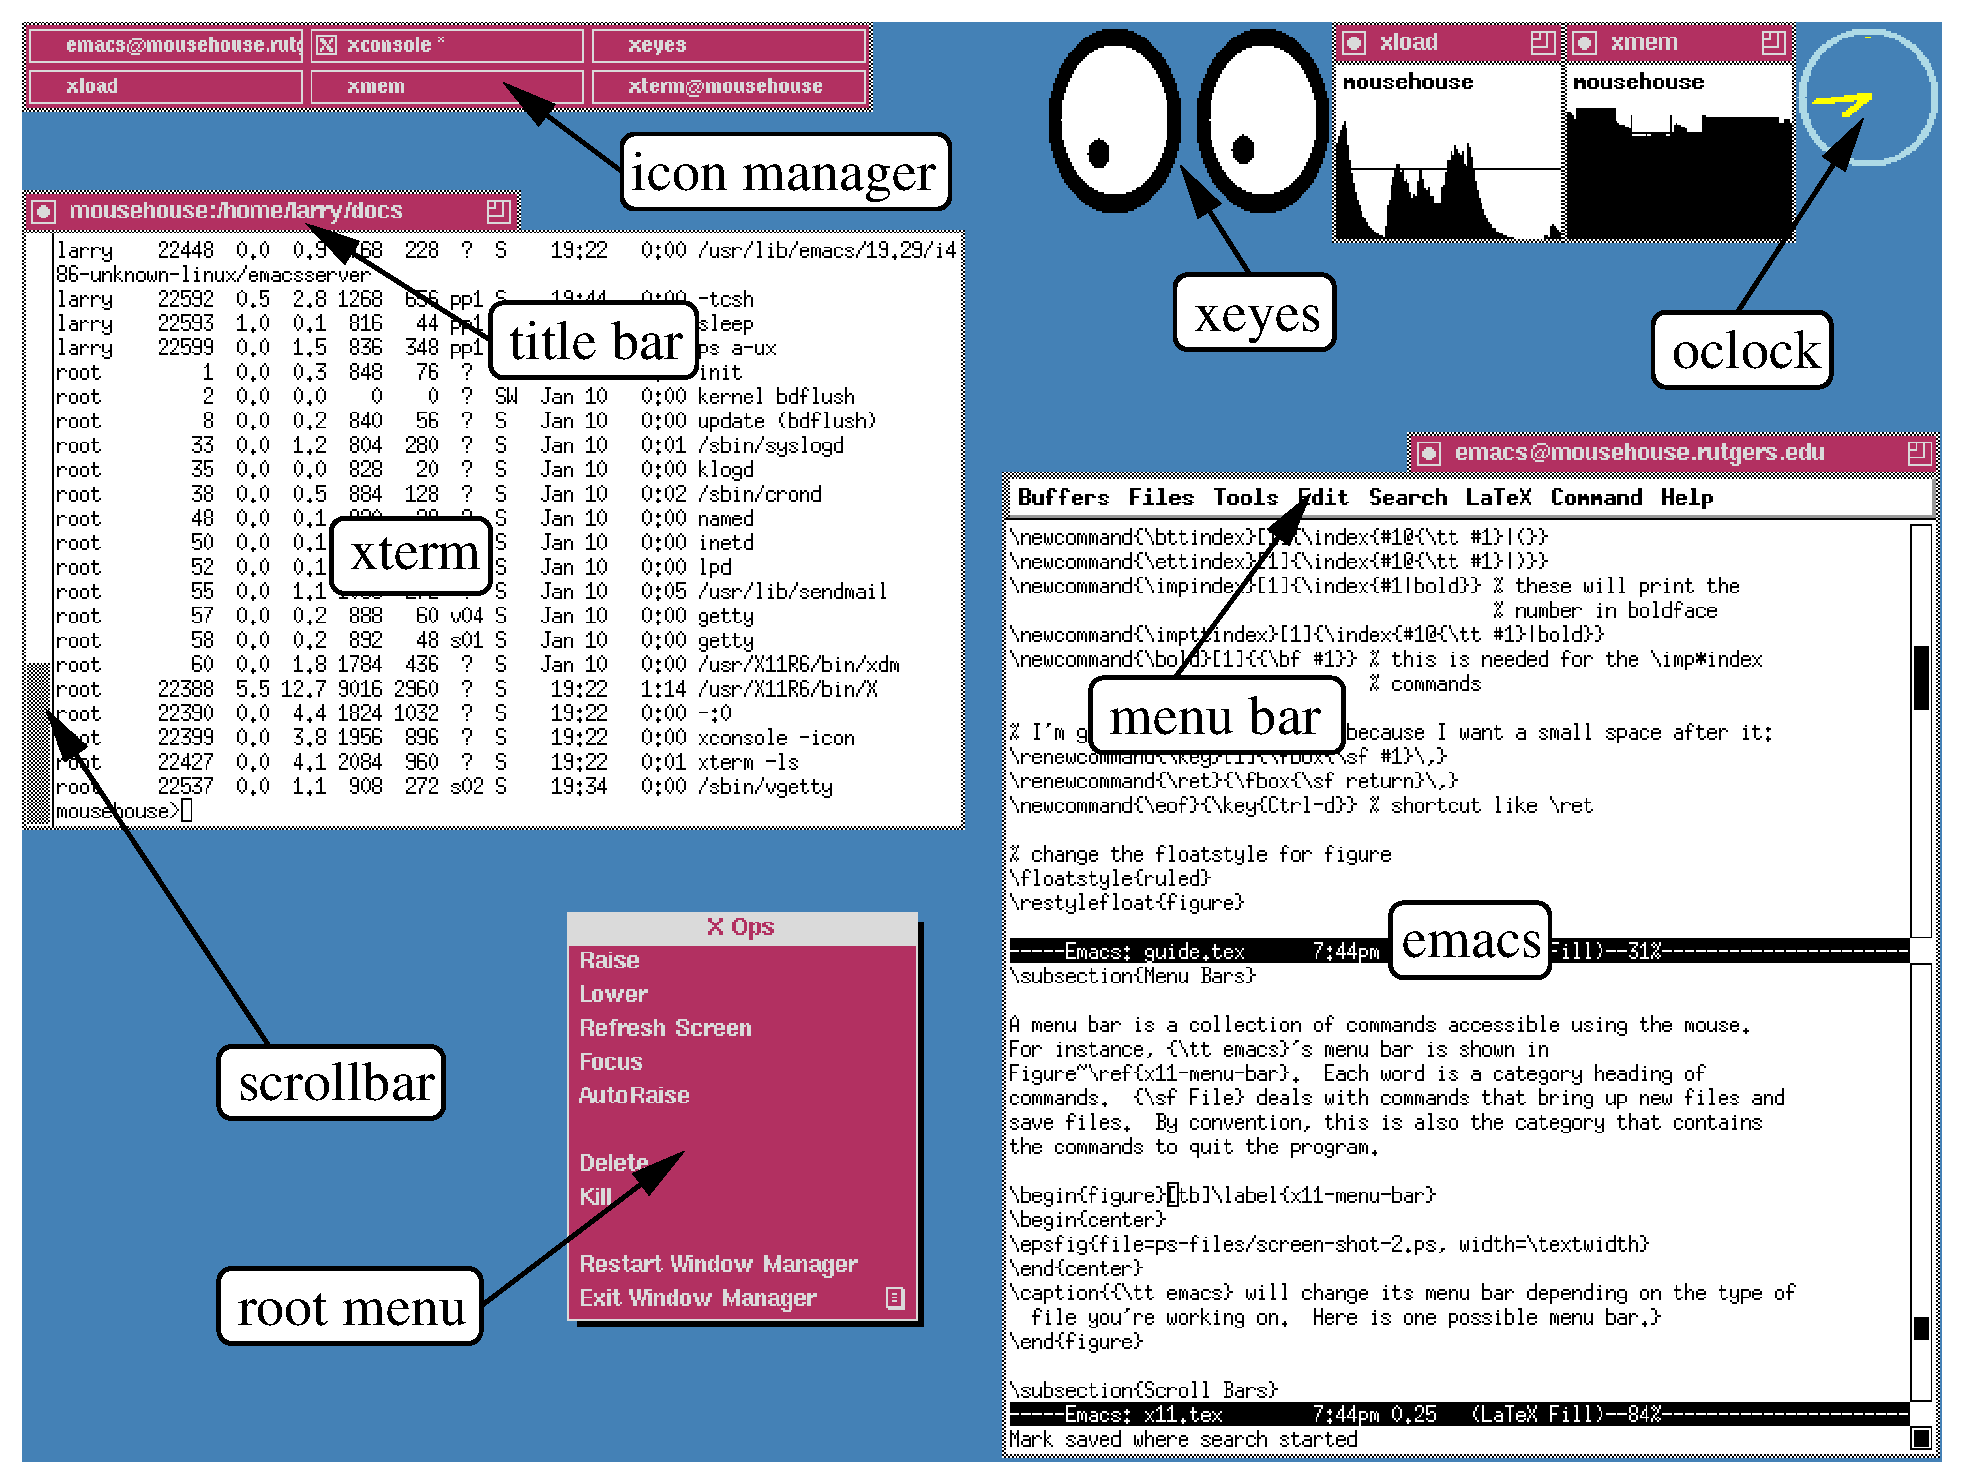
\epsfig{file=ps-files/screen-shot-5.ps, width=\linewidth}
\caption{An annotated example of a standard X screen.  In this
 example, the user is running {\tt twm}.  The standard clock has been
  replaced by a transparent clock called {\tt oclock}.}
\end{figure}

\subsection{XClock}

\begin{command}
{\tt xclock} [-digital] [-analog] [-update {\sl seconds}] [-hands {\sl
  color}]
\end{command}

I'll explain the simpliest one first: {\tt xclock}\ttindex{xclock}
functions exactly as you'd expect it would.  It ticks off the seconds,
minutes and hours in a small window.

No amounts of clicking or typing in {\tt xclock}'s window will affect
it---that's {\em all\/} it does. Or is it? In fact, there are various
different options you can give to the program to have it act in
different ways. For instance, {\tt xclock -digital} will create a
digital clock. {\tt xclock -update 1} will create a second hand that
moves every second, while {\tt -update 5} will create a second hand
that moves every 5 seconds.

For more information on {\tt xclock}'s options, consult its
manpage---{\tt man xclock}. If you're going to try running a few of
your own {\tt xclock}s, you should probably read
Section~\ref{section-multitasking} (Multitasking) to learn how to run
them in addition to your current programs.  (If you run an {\tt
  xclock} in the foreground---the usual way of running a program---and
want to get out of it, type \key{ctrl-c}.)

\subsection{XTerm} % better section name?

The window with a prompt in it (something that probably looks like
{\tt /home/larry\#}) is being controlled by a program called {\tt
  xterm}\impttindex{xterm}.  {\tt xterm} is a deceptively complicated
program.  At first glance, it doesn't seem to do much, but it actually
has to do a lot of work.  {\tt xterm} emulates a terminal so that
regular text-mode \unix\ applications work correctly.  It also
maintains a buffer of information so that you can refer back to old
commands.  (To see how to use this, look at
Section~\ref{x-scroll-bar}.)

For much of this book, we're going to be learning about the \unix\ 
command-line, and you'll find that inside your {\tt xterm} window.
In order to type into {\tt xterm}, you {\em usually\/} have to move
your mouse cursor (possibly shaped like an ``X'' or an arrow) into the
{\tt xterm} window.  However, this behavior is dependent on the window
manager.

One way of starting more programs under X is through an {\tt xterm}.
Since X programs are standard \unix\ programs, they can be run from
normal command prompts such as {\tt xterm}s.  Since running a long
term program from a {\tt xterm} would tie up the {\tt xterm} as long
as the program was running, people normally start X programs in the
background.  For more information about this, see
Section~\ref{section-multitasking}.

\section{Window Managers}

On \linux, there are two different window managers that are commonly
used.  One of them, called {\tt twm}\ttindex{twm} is short for ``Tab
Window Manager''. % this is from the manpage. is it correct?
It is larger than the other window manager usually used, {\tt fvwm}.
({\tt fvwm} stands for ``F(?) Virtual Window Manager''---the author
neglected to tie down exactly what the f stood for.)  Both {\tt twm}
and {\tt fvwm} are highly configurable, which means I can't tell you
exactly what keys do what in your particular setup.

To learn about {\tt twm}'s configuration, look at
Section~\ref{twm-config-section}. {\tt fvwm}'s configuration is
covered in Section~\ref{fvwm-config-section}.

\subsection{When New Windows are Created}

There are three possible things a window manager will do when a new
window is created.  It is possible to configure a window manager so
that an outline of the new window is shown, and you are allowed to
position it on your screen. That is called \concept{manual placement}.
If you are presented with the outline of a window, simply use the
mouse to place it where you wish it to appear and click the left mouse
button.

It is also possible that the window manager will place the new window
somewhere on the screen by itself.  This is known as 
\concept{random placement}.

Finally, sometimes an application will ask for a specific spot on the
screen, or the window manager will be configured to display certain
applications on the same place of the screen all the time. (For
instance, I specify that I want {\tt xclock} to always appear in
the upper right hand corner of the screen.)

\subsection{Focus}

The window manager controls some important things. The first thing
you'll be interested in is \concept{focus}.  The focus of the server is
which window will get what you type into the keyboard. Usually in X
the focus is determined by the position of the mouse cursor.  If the
mouse cursor is in one {\tt xterm}'s window\footnote{You can have more
  then one copy of {\tt xterm} running at the same time!}, that {\tt
  xterm} will get your keypresses.  This is different from many other
windowing systems, such as Microsoft Windows, OS/2, or the Macintosh,
where you must click the mouse in a window before that window gets
focus.  Usually under X, if your mouse cursor wanders from a
window, focus will be lost and you'll no longer be able to type there.

Note, however, that it is possible to configure both {\tt
  twm}\ttindex{twm} and {\tt fvwm}\ttindex{fvwm} so that you must
click on or in a window to gain focus, and click somewhere else to
lose it, identical to the behavior of Microsoft Windows.  Either
discover how your window manager is configured by trial and error, or
consult local documentation.

\subsection{Moving Windows}

Another very configurable thing in X is how to move windows around.
In my personal configuration of {\tt twm}, there are three different
ways of moving windows around.  The most obvious method is to move the
mouse cursor onto the \concept{title bar} and drag the window around
the screen. Unfortunately, this may be done with any of the left,
right, or middle buttons\footnote{Many PCs have only two button mice.
  If this is the case for you, you should be able to emulate a middle
  button by using the left and right buttons simultaneously.}. (To
drag, move the cursor above the title bar, and hold down on the button
while moving the mouse.)  Most likely, your configuration is
set to move windows using the \emph{left} mouse buttons.

Another way of moving windows may be holding down a key while dragging
the mouse. For instance, in {\em my\/} configuration, if I hold down
the \key{Alt} key, move the cursor above a window, I can drag the
window around using the left mouse button.

Again, you may be able to understand how the window manager is
configured by trial and error, or by seeing local
documentation. Alternatively, if you want to try to interpret the
window manager's configuration file, see
Section~\ref{twm-config-section} for {\tt twm}\ttindex{twm} or
Section~\ref{fvwm-config-section} for {\tt fvwm}\ttindex{fvwm}.

\subsection{Depth}

Since windows are allowed to overlap in X, there is a concept of
\concept{depth}.  Even though the windows and the screen are both two
dimensional, one window can be in front of another, partially or
completely obscuring the rear window.

There are several operations that deal with depth:
\begin{itemize}
\item {\bf Raising} the window, or bringing a window to the front.
  This is usually accomplished by clicking on a window's title bar
  with one of the buttons.  Depending on how the window manager is
  configured, it could be any one of the buttons. (It is also possible
  that more then one button will do the job.)

\item {\bf Lowering} the window, or pushing the window to the back.
  This can generally be accomplished by a different click in the title
  bar. It is also possible to configure some window managers so that
  one click will bring the window foward if there is anything over it,
  while that same click will lower it when it is in the front.

\item {\bf Cycling} through windows is another operation many window
  managers allow. This brings each window to the front in an orderly
  cycle.  
\end{itemize}

\subsection{Iconization}

There are several other operations that can obscure windows or hide
them completely. First is the idea of ``iconization''. Depending on
the window manager, this can be done in many different ways. In {\tt
  twm}, many people configure an {\bf icon manager}\index{icon
  manager}. This is a special window that contains a list of all the
other windows on the screen.  If you click on a name (depending on the
setup, it could be with any of the buttons!) the window
disappears---it is iconified.  The window is still active, but you
can't see it.  Another click in the icon manager restores the window
to the screen.

This is quite useful.  For instance, you could have remote {\tt
  xterm}s to many different computers that you occasionally use.
However, since you rarely use all of them at a given time, you can
keep most of the {\tt xterm} windows iconified while you work with a
small subset. The only problem with this is it becomes easy to
``lose'' windows. This causes you to create new windows that duplicate
the functionality of iconified windows.

Other window managers might create actual icons across the bottom of
the screen, or might just leave icons on the root
window.\glossary{root window}

\subsection{Resizing}

There are several different methods to resize windows under X.  Again,
it is dependent on your window manager and exactly how your window
manager is configured.  The method many Microsoft Windows users are
familiar with is to click on and drag the border of a window.  If your
window manager creates large borders that change how the mouse cursor
looks when it is moved over them, that is probably the method used to
resize windows.

Another method used is to create a ``resizing'' button on the
titlebar.  In Figure~\ref{full-x-screen}, a small button is visible on
the right of each titlebar.  To resize windows, the mouse is moved
onto the resize button and the left mouse button is held down.  You
can then move the mouse outside the borders of the window to resize
it.  The button is released when the desired size has been reached.

\subsection{Maximization}

Most window managers support maximization.  In {\tt twm}, for
instance, you can maximize the height, the width, or both dimensions
of a window. This is called ``zooming'' in {\tt twm}'s language
although I prefer the term maximization.  Different applications
respond differently to changes in their window size. (For instance,
{\tt xterm} won't make the font bigger but will give you a larger
workspace.)

Unfortunately, it is extremely non-standard on how to maximize windows.

\subsection{Menus}\label{x-menus}

Another purpose for window managers is for them to provide menus for
the user to quickly accomplish tasks that are done over and over.  For
instance, I might make a menu choice that automatically launches Emacs
or an additional {\tt xterm} for me. That way I don't need to type in
an {\tt xterm}---an especially good thing if there aren't any running
{\tt xterm}s that I need to type in to start a new program!

In general, different menus can be accessed by clicking on the root
window, which is an immovable window behind all the other ones. By
default, it is colored gray, but could look like
anything.\footnote{One fun program to try is called {\tt
    xfishtank}\ttindex{xfishtank}.  It places a small aquarium in the
  background for you.} To try to see a menu, click and hold down a
button on the desktop. A menu should pop up. To make a selection, move
(without releasing the mouse button) the cursor over one of the items
any then release the mouse button.

\section{X Attributes}

There are many programs that take advantage of X. Some programs, like
{\tt emacs}\ttindex{emacs}, can be run either as a text-mode program
{\em or\/} as a program that creates its own X window. However, most X
programs can only be run under X.

\subsection{Geometry}\index{X Window System!geometry}

There are a few things common to all programs running under X.  In X, the
concept of {\bf geometry} is where and how large a window is.  A
window's geometry has four components:
\begin{itemize}
\item The horizontal size, usually measured in pixels. (A pixel is the
  smallest unit that can be colored. Many X setups on Intel PCs have
  1024 pixels horizontally and 768 pixels vertically.) Some
  applications, like {\tt xterm} and {\tt emacs}, measure their size in
  terms of number of characters they can fit in the window. (For
  instance, eighty characters across.)
\item The vertical size, also usually measured in pixels. It's
  possible for it to be measured in characters.
\item The horizontal distance from one of the sides of the screen. For
  instance, {\tt +35} would mean make the left edge of the window
  thirty-five pixels from the left edge of the screen. On the other
  hand, {\tt -50} would mean make the right edge of the window fifty
  pixels from the right edge of the screen.  It's generally impossible to start
  the window off the screen, although a window can be moved off the
  screen.  (The main exception is when the window is very large.)
\item The vertical distance from either the top or the bottom. A
  positive vertical distance is measured from the top of the screen; a
  negative vertical distance is measured from the bottom of the
  screen.
\end{itemize}

All four components get put together into a geometry string that looks
like: {\tt 503x73-78+0}. (That translates into a window 503 pixels
long, 73 pixels high, put near the top right hand corner of the
screen.)  Another way of stating it is {\sl hsize\/}{\tt x}{\sl
  vsize\/}$\pm${\sl hplace\/}$\pm${\sl vplace\/}.

\subsection{Display}

Every X application has a display that it is associated with.  The
display is the name of the screen that the X server controls.  A
display consists of three components:

\begin{itemize}
\item The machine name that the server is running on.  At stand-alone
  \linux\ installations the server is always running on the same
  system as the clients. In such cases, the machine name can be
  omitted.
\item The number of the server running on that machine. Since any one
  machine could have multiple X servers running on it (unlikely for
  most \linux\ machines, but possible) each must have a unique number.
\item The screen number.  X supports a particular server controlling
  more than one screen at a time. You can imagine that someone wants a
  lot of screen space, so they have two monitors sitting next to each
  other. Since they don't want two X servers running on one machine
  for performance reasons, they let one X server control both screens.
\end{itemize}

These three things are put together like so: {\sl machine\/}:{\sl
  server-number\/}.{\sl screen-number\/}.

For instance, on {\tt mousehouse}, all my applications have the
display set to {\tt :0.0}, which means the first screen of the first
server on the local display. However, if I am using a remote computer,
the display might be set to {\tt mousehouse:0.0}.

By default, the display is taken from the environment variable (see
Section~\ref{section-env-variables}) named {\tt DISPLAY}, and can be
overridden with a command-line option (see
Figure~\ref{x-standard-options}). To see how {\tt DISPLAY} is set, try
the command {\tt echo \$DISPLAY}.

\begin{figure}
\begin{center}
\begin{tabular}{|l|p{.4\linewidth}|p{.4\linewidth}|}\hline
  Name & Followed by & Example\\ \hline
{\tt -geometry} & geometry of the window & {\tt xterm
  -geometry 80x24+0+90}\\ \hline
{\tt -display}  & display you want the program to appear &
                  {\tt xterm -display lionsden:0.0}\\ \hline
{\tt -fg} & the primary foreground color & {\tt xterm -fg
  yellow}\\ \hline
{\tt -bg} & the primary background color & {\tt xterm -bg blue}\\ \hline
\end{tabular}
\end{center}
\caption{Standard options for X programs.}\label{x-standard-options}
\end{figure}

\section{Common Features}

While X is a graphical user interface, it is a very uneven graphical
user interface.  It's impossible to say how any component of the
system is going to work, because every component can easily be
reconfigured, changed, and even replaced. This means it's hard to say
exactly how to use various parts of the interface.  We've already
encountered one cause of this: the different window managers and how
configurable each window manager is.

Another cause of this uneven interface is the fact that X applications
are built using things called ``widget sets''.  Included with the
standard X distribution are ``Athena widgets'' developed at MIT.
These are commonly used in free applications.  They have the
disadvantage that they are not particularly good-looking and are
somewhat harder to use than other widgets.\index{X Window
  System!Athena Widget Set}

The other popular widget set is called 
``Motif''.\index{X Window System!Motif Widget Set} Motif is a
commercial widget set similar to the user interface used in Microsoft
Windows.  Many commercial applications use Motif widgets, as well as
some free applications.  The popular World Wide Web Browser {\tt
  netscape}\ttindex{netscape} uses Motif.

Let's try to go through some of the more usually things you'll
encounter.

\subsection{Buttons}

Buttons are generally the easiest thing to use.  A button is invoked
by positioning the mouse cursor over it and clicking (pressing and
immediately releasing the mouse button) the left button.  Athena and
Motif buttons are functionally the same although they have cosmetic
differences.

\subsection{Menu Bars}

A menu bar is a collection of commands accessible using the mouse.
For instance, {\tt emacs}'s menu bar is shown in
Figure~\ref{x11-menu-bar}.  Each word is a category heading of
commands.  {\sf File} deals with commands that bring up new files and
save files.  By convention, this is also the category that contains
the command to exit the program.

To access a command, move the mouse cursor over a particular category
(such as {\sf File}) and press and hold down the left mouse button.
This will display a variety of commands.  To select one of the
commands, move the mouse cursor over that command and release the left
mouse button.  Some menu bars let you click on a category---if this is
the case, clicking on the category will display the menu until you
click on either a command, another menu, or outside the menu bar
(indicating that you are not interested in running a particular
command).

\begin{figure}[tb]
\begin{center}
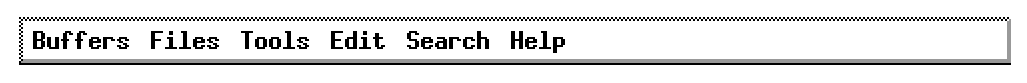
\epsfig{file=ps-files/screen-shot-2.ps, width=\textwidth}
\end{center}
\caption{{\tt emacs} will change its menu bar depending on the type of
  file you're working on.  Here is one possible menu
  bar.}\label{x11-menu-bar}
\end{figure}

\subsection{Scroll Bars}\label{x-scroll-bar}

A {\bf scroll bar} is a method to allow people to display only part of
a document, while the rest is off the screen.  For instance, the {\tt
  xterm} window is currently displaying the bottom third of the text
available in Figure~\ref{x11-scrollbar}.  It's easy to see what part
of the available text is current being displayed: the darkened part of
the scroll bar is relative to both the position and the amount of
displayed text.  If the text displayed is all there is, the entire
scroll bar is dark.  If the middle half of the text is displayed, the
middle half of the scroll bar is darkened.\index{X Window System!scrollbar}

A vertical scroll bar may be to the left or right of the text and a
horizontal one may be above or below, depending the application.

\begin{figure}[tb]
\begin{center}
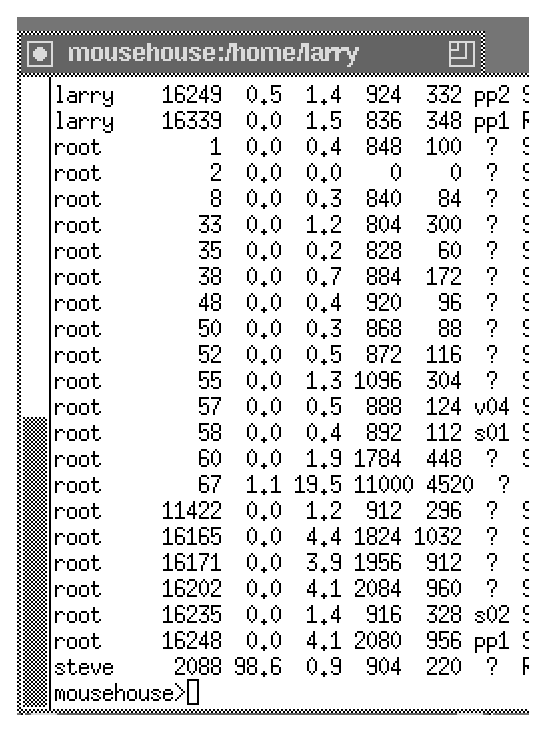
\epsfig{file=ps-files/screen-shot-3.ps, height=3in} \hspace{0.7in}

\epsfig{file=ps-files/screen-shot-4.ps, height=3in}
\end{center}
\caption{An Athena-type scroll bar is visible on the left of this {\tt
    xterm} window.  Next to it, a Motif-type scroll bar is visible on
  the {\tt netscape} window.}\label{x11-scrollbar}
\end{figure}


\subsubsection{Athena scroll bars}

Athena scroll bars operate differently from scroll bars in other
windowing systems.  Each of the three buttons of the mouse operate
differently.  To scroll upwards (that is, display material above what
is currently visible) you can click the rightmost mouse button
anywhere in the scroll bar.  To scroll downwards, click the left mouse
button anywhere in the scroll bar.

You can also jump to a particular location in the displayed material
by clicking the middle mouse button anywhere in the scroll bar.  This
causes the window to display material starting at that point in the
document.

\subsubsection{Motif scroll bars}

A Motif scroll bar acts much more like a Microsoft Windows or
Macintosh scroll bar.  An example of one is on the right in
Figure~\ref{x11-scrollbar}.  Notice that in addition to the bar, it
has arrows above and below it.  These are used for fine-tuning:
clicking either the left or middle buttons on them will scroll a small
amount such as one line; the right button does nothing.

The behavior of clicking inside the scroll bar is widely different for
Motif scroll bars than Athena scroll bars.  The right button has no
effect.  Clicking the left button above the current position scrolls
upward.  Similarly, clicking below the current position scrolls
downward.  Clicking and holding the left button \emph{on} the current
position allows one to move the bar at will.  Releasing the left
button positions the window.

Clicking the middle button anywhere on the bar will immediately jump
to that location, similar to the behavior of the Athena middle
button.  However, instead of starting to display the data at the
position clicked, that position is taken to be the \emph{midpoint} of
the data to be displayed.

\eindex{X Window System}
% Local Variables: 
% mode: latex
% TeX-master: "guide"
% End: 


% more advance shell stuff: piping, redirection, filters, more
% commands
\chapter{Working with \unix}\label{shell2-chapter}


\begin{fortune}
\begin{verse}
A UNIX saleslady, Lenore,\\
Enjoys work, but she likes the beach more.\\
\hspace{0.5in}She found a good way\\
\hspace{0.5in}To combine work and play:\\
She sells C shells by the seashore.
\end{verse}
\end{fortune}
\glossary{C shell}\glossary{Bourne shell}
\glossary{file}\glossary{input}\glossary{output}


\unix\ is a powerful system for those who know how to harness its
power.  In this chapter, I'll try to describe various ways to use
\unix's shell, {\tt bash}\ttindex{bash}, more efficently.

\section{Wildcards}\bindex{shell!wildcards}
\index{shell!globbing|see{shell, wildcards}}
\index{wildcards|see{shell, wildcards}}

In the previous chapter, you learned about the file maintence commands {\tt
cp}, {\tt mv}, and {\tt rm}.  Occasionally, you want to deal with more than
one file at once---in fact, you might want to deal with many files at once.
For instance, you might want to copy all the files beginning with {\tt
data} into a directory called {\tt \verb+~+/backup}.  You could do this by either
running many {\tt cp} commands, or you could list every file on one command
line. Both of these methods would take a long time, however, and you have a
large chance of making an error.

A better way of doing that task is to type:
\begin{screen}\begin{verbatim}
/home/larry/report# ls -F
1993-1          1994-1          data1           data5
1993-2          data-new        data2
/home/larry/report# mkdir ~/backup
/home/larry/report# cp data* ~/backup
/home/larry/report# ls -F ~/backup
data-new        data1           data2           data5
/home/larry/report#
\end{verbatim}\end{screen}

As you can see, the asterix told {\tt cp} to take all of the files
beginning with {\tt data} and copy them to {\tt \verb+~+/backup}. Can you guess
what {\tt cp d*w \verb+~+/backup} would have done?

\subsection{What {\em Really\/} Happens?}

Good question. Actually, there are a couple of special characters
intercepted by the shell, {\tt bash}\ttindex{bash}. The character
``{\tt *}'', an asterix, says ``replace this word with all the files
that will fit this specification''. So, the command {\tt cp data*
  \verb+~+/backup}, like the one above, gets changed to {\tt cp
  data-new data1 data2 data5 \verb+~+/backup} before it gets run.

To illustrate this, let me introduce a new command, {\tt
  echo}\impttindex{echo}. {\tt echo} is an extremely simple command;
it echoes back, or prints out, any parameters. Thus:

\begin{screen}\begin{verbatim}
/home/larry# echo Hello!
Hello!
/home/larry# echo How are you?
How are you?
/home/larry# cd report
/home/larry/report# ls -F
1993-1          1994-1          data1           data5
1993-2          data-new        data2
/home/larry/report# echo 199*
1993-1 1993-2 1994-1
/home/larry/report# echo *4*
1994-1
/home/larry/report# echo *2*
1993-2 data2
/home/larry/report#
\end{verbatim}
\end{screen}

As you can see, the shell expands the wildcard and passes all of the
files to the program you tell it to run. This raises an interesting
question: what happens if there are {\em no\/} files that meet the
wildcard specification? Try {\tt echo /rc/fr*og} and {\tt
  bash}\ttindex{bash} passes the wildcard specification verbatim to
the program.

Other shells, like {\tt tcsh}\ttindex{tcsh}, will, instead of just
passing the wildcard verbatim, will reply {\tt No match.} Here's the
same command run under {\tt tcsh}:

\begin{screen}\begin{verbatim}
mousehouse>echo /rc/fr*og
echo: No match.
mousehouse>
\end{verbatim}\end{screen}

The last question you might want to know is what if I wanted to have
{\tt data*} echoed back at me, instead of the list of file names?
Well, under both {\tt bash} and {\tt tcsh}, just include the string in
quotes:

\begin{minipage}{2.6in}\begin{screen}
\begin{verbatim}
/home/larry/report# echo "data*"
data*
/home/larry/report#
\end{verbatim}\end{screen}\end{minipage}\ {\large OR}\ 
\begin{minipage}{2.6in}\begin{screen}
\begin{verbatim}
mousehouse>echo "data*"
data*
mousehouse>
\end{verbatim}\end{screen}\end{minipage}

\subsection{The Question Mark}

In addition to the asterix, the shell also interprets a question mark
as a special character.  A question mark will match one, and only one
character. For instance, {\tt ls /etc/??} will display all two letter
files in the the {\tt /etc} directory.

\eindex{shell!wildcards}

\section{Time Saving with {\tt bash}}
\index{command line editing|see{shell, editing}}

\subsection{Command-Line Editing}\bindex{shell!editing}

Occasionally, you've typed a long command to {\tt bash}\ttindex{bash} and,
before you hit return, notice that there was a spelling mistake early in
the line.  You could just delete all the way back and retype everything you
need to, but that takes much too much effort! Instead, you can use the
arrow keys to move back there, delete the bad character or two, and type
the correct information.

There are many special keys to help you edit your command line, most of
them similar to the commands used in GNU Emacs\index{GNU Emacs}. For
instance, \key{C-t} flips two adjacent characters.\footnote{\key{C-t} means
hold down the key labeled ``Ctrl'', then press the ``t'' key. Then release
the ``Ctrl'' key.} You'll be able to find most of the commands in the
chapter on Emacs, Chapter~\ref{emacs-chapter}.

\eindex{shell!editing}

\subsection{Command and File Completion}\bindex{shell!completion}

Another feature of {\tt bash}\ttindex{bash} is automatic completion of
your command lines.  For instance, let's look at the following example
of a typical {\tt cp} command:

\begin{screen}\begin{verbatim}
/home/larry# ls -F
this-is-a-long-file
/home/larry# cp this-is-a-long-file shorter
/home/larry# ls -F
shorter              this-is-a-long-file
/home/larry# 
\end{verbatim}\end{screen}

It's a big pain to have to type every letter of {\tt
  this-is-a-long-file} whenever you try to access it.  So, create {\tt
  this-is-a-long-file} by copying {\tt /etc/passwd} to it\footnote{\tt cp
  /etc/passwd this-is-a-long-file}. Now, we're going to do the above {\tt
  cp} command very quickly and with a smaller chance of mistyping.

Instead of typing the whole filename, type {\tt cp th} and press and
release the \key{Tab}. Like magic, the rest of the filename shows up
on the command line, and you can type in {\tt shorter}. Unfortunately,
{\tt bash}\ttindex{bash} cannot read your thoughts, and you'll have to
type all of {\tt shorter}.

When you type \key{Tab}, {\tt bash} looks at what you've typed and
looks for a file that starts like that. For instance, if I type {\tt
  /usr/bin/ema} and then hit \key{Tab}, {\tt bash} will find {\tt
  /usr/bin/emacs} since that's the only file that begins {\tt
  /usr/bin/ema} on my system. However, if I type {\tt /usr/bin/ld} and
hit \key{Tab}, {\tt bash} beeps at me. That's because three files,
{\tt /usr/bin/ld}, {\tt /usr/bin/ldd}, and {\tt /usr/bin/ld86} all
start with {\tt /usr/bin/ld} on my system.

If you try a completion and {\tt bash} beeps, you can immediately hit
\key{Tab} again to get a list of all the files your start matches so
far. That way, if you aren't sure of the exact spelling of your file,
you can start it and scan a much smaller list of files.

\eindex{shell!completion}

\section{The Standard Input and The Standard Output}

% it might be nice to get some illustrations around here, with
% pointers showing where all the output is going

Let's try to tackle a simple problem: getting a listing of the {\tt
  /usr/bin} directory. If all we do is {\tt ls /usr/bin}, some of the
files scroll off the top of the screen. How can we see all of the
files?

\subsection{\unix\ Concepts}

The \unix\ operating system makes it very easy for programs to use the
terminal.  When a program writes something to your screen, it is using
something called \concept{standard output}.  Standard output,
abbreviated as stdout, is how the program writes things to a user. The
name for what you tell a program is \concept{standard input} (stdin).
It's possible for a program to communicate with the user without using
standard input or output, but most of the commands I cover in this
book use stdin and stdout.

For example, the {\tt ls}\ttindex{ls} command prints the list of the
directories to standard output, which is normally ``connected'' to
your terminal.  An interactive command, such as your shell, {\tt
  bash}\ttindex{bash}, reads your commands from standard input.

It is also possible for a program to write to 
\concept{standard error}, since it is very easy to make standard
output point somewhere besides your terminal. Standard error (stderr)
is almost always connected to a terminal so an actual human will read
the message.

In this section, we're going to examine three ways of fiddling with
the standard input and output: input redirection, output redirection,
and pipes.

\subsection{Output Redirection}\bindex{output redirection}

A very important feature of \unix\ is the ability to {\bf redirect}
output. This allows you, instead of viewing the results of a command,
to save it in a file or send it directly to a printer. For instance,
to redirect the output of the command {\tt ls /usr/bin}, we place a
{\tt >} sign at the end of the line, and say what file we want the
output to be put in:

\begin{screen}\begin{verbatim}
/home/larry# ls
/home/larry# ls -F /usr/bin > listing
/home/larry# ls
listing
/home/larry#
\end{verbatim}\end{screen}

As you can see, instead of writing the names of all the files, the
command created a totally new file in your home directory. Let's try
to take a look at this file using the command {\tt cat}. If you think
back, you'll remember {\tt cat} was a fairly useless command that
copied what you typed (the standard input) to the terminal (the
standard output). {\tt cat} can also print a file to the standard
output if you list the file as a parameter to {\tt cat}:

\begin{screen}\begin{verbatim}
/home/larry# cat listing
...
/home/larry#
\end{verbatim}\end{screen}

The exact output of the command {\tt ls /usr/bin} appeared in the
contents of {\tt listing}. All well and good, although it didn't solve
the original problem.\footnote{For impatient readers, the command you
  might want to try is {\tt more}. However, there's still a bit more
  to talk about before we get there.}

However, {\tt cat} does do some interesting things when it's output is
redirected. What does the command {\tt cat listing > newfile} do?
Normally, the {\tt > newfile} says ``take all the output of the
command and put it in {\tt newfile}.'' The output of the command {\tt
  cat listing} is the file {\tt listing}. So we've invented a new (and
not so efficient) method of copying files.

How about the command {\tt cat > fox}? {\tt cat} by itself reads in
each line typed at the terminal (standard input) and prints it right
back out (standard output) until it reads \key{Ctrl-d}. In this case,
standard output has been redirected into the file {\tt fox}. Now {\tt
  cat} is serving as a rudimentary editor:

\begin{quote}{\tt 
/home/larry\# cat > fox\\
The quick brown fox jumps over the lazy dog.\\
{\em press Ctrl-d}
}\end{quote}

We've now created the file {\tt fox} that contains the sentence ``The
quick brown fox jumps over the lazy dog.'' One last use of the
versitile {\tt cat} command is to con{\bf cat}enate files together.
{\tt cat} will print out every file it was given as a parameter, one
after another. So the command {\tt cat listing fox} will print out the
directory listing of {\tt /usr/bin}, and then it will print out our
silly sentence. Thus, the command {\tt cat listing fox > listandfox}
will create a new file containing the contents of both {\tt listing}
and {\tt fox}.

\eindex{output redirection}

\subsection{Input Redirection}\bindex{input redirection}

Like redirecting standard output\index{standard output}, it is also
possible to redirect standard input\index{standard input}. Instead of
a program reading from your keyboard, it will read from a file.  Since
input redirection is related to output redirection, it seems natural
to make the special character for input redirection be {\tt <}. It
too, is used after the command you wish to run.

This is generally useful if you have a data file and a command that
expects input from standard input.  Most commands also let you specify
a file to operate on, so {\tt <} isn't used as much in day-to-day
operations as other techniques.

\eindex{input redirection}

\subsection{The Pipe}\bindex{pipes}

Many \unix\ commands produce a large amount of information. For instance,
it is not uncommon for a command like {\tt ls /usr/bin} to produce more
output than you can see on your screen. In order for you to be able to see
all of the information that a command like {\tt ls /usr/bin}, it's
necessary to use another \unix\ command, called {\tt
more}\ttindex{more}.\footnote{{\tt more}\ttindex{more} is named because
that's the prompt it originally displayed: {\tt --more--}. In many versions
of \linux\ the {\tt more} command is identical to a more advanced command
that does all that {\tt more} can do and more. Proving that computer
programmers make bad comedians, they named this new program {\tt
less}\ttindex{less}.} {\tt more} will pause once every screenful
of information. For instance, {\tt more < /etc/rc} will display the file
{\tt /etc/rc} just like {\tt cat /etc/rc} would, except that {\tt more}
will let you read it.  {\tt more} also allows the command {\tt more
/etc/rc}, and that's the normal way of invoking it.

However, that doesn't help the problem that {\tt ls /usr/bin} displays more
information than you can see. {\tt more < ls /usr/bin} won't work---input
redirection only works with files, not commands! You {\em could\/} do this:

\begin{screen}\begin{verbatim}
/home/larry# ls /usr/bin > temp-ls
/home/larry# more temp-ls
...
/home/larry# rm temp-ls
\end{verbatim}\end{screen}

However, \unix\ supplies a much cleaner way of doing that. You can just use
the command {\tt ls /usr/bin | more}. The character ``{\tt |}'' indicates a
{\bf pipe}. Like a water pipe, a \unix\ pipe controls flow. Instead of
water, we're controlling the flow of information!

A useful tool with pipes are programs called {\bf
  filters}\index{filters}.  A filter is a program that reads the
standard input, changes it in some way, and outputs to standard
output. {\tt more} is a filter---it reads the data that it gets from
standard input and displays it to standard output one screen at a
time, letting you read the file.  {\tt more} isn't a great filter
because its output isn't suitable for sending to another program.

Other filters include the programs {\tt cat}\ttindex{cat}, {\tt
sort}\ttindex{sort}, {\tt head}\ttindex{head}, and {\tt
tail}\ttindex{tail}. For instance, if you wanted to read only the first ten
lines of the output from {\tt ls}, you could use {\tt ls /usr/bin | head}.

\eindex{pipes}

\section{Multitasking}\label{section-multitasking}

\subsection{Using Job Control}
\index{job control|see{shell, job control}} 

{\bf Job control}\index{shell!job control} refers to the ability to
put processes (another word for programs, essentially) in the
\concept{background} and bring them to the \concept{foreground} again.
That is to say, you want to be able to make something run while you go
and do other things, but have it be there again when you want to tell
it something or stop it.  In Unix, the main tool for job control is
the shell---it will keep track of jobs for you, if you learn how to
speak its language.

        The two most important words in that language are {\tt
fg}\ttindex{fg}, for foreground, and {\tt bg}\ttindex{bg}, for
background.  To find out how they work, use the command \ttindex{yes}
{\tt yes} at a prompt.

\begin{screen}\begin{verbatim}
/home/larry# yes
\end{verbatim}
\end{screen}

This will have the startling effect of running a long column of {\tt
  y}'s down the left hand side of your screen, faster than you can
follow.\footnote{There are good reasons for this strange command to
  exist.  Occasional commands ask for confirmation---a ``yes'' answer
  to a question.  The {\tt yes} command allows a programmer to
  automate the response to these questions.} To get them to stop,
you'd normally type \key{ctrl-c} to kill it, but instead you should
type \key{ctrl-z} this time.  It appears to have stopped, but there
will be a message before your prompt, looking more or less like this:

\begin{screen}\begin{verbatim}
[1]+   Stopped                  yes
\end{verbatim}
\end{screen}

It means that the process {\tt yes} has been \concept{suspended} in
the background.  You can get it running again by typing \ttindex{fg}
\index{foreground} {\tt fg} at the prompt, which will put it into the
foreground again.  If you wish, you can do other things first, while
it's suspended.  Try a few {\tt ls}'s or something before you put it
back in the foreground.

        Once it's returned to the foreground, the {\tt y}'s will start
coming again, as fast as before.  You do not need to worry that while
you had it suspended it was ``storing up'' more {\tt y}'s to send to the
screen: when a program is suspended the whole program doesn't run
until you bring it back to life.  (Now type \key{ctrl-c} to
kill it for good, once you've seen enough).

        Let's pick apart that message we got from the shell:

\begin{screen}\begin{verbatim}
[1]+   Stopped                yes
\end{verbatim}\end{screen}

        The number in brackets is the \index{shell!job number} {\bf job
number} of this job, and will be used when we need to refer to it
specifically.  (Naturally, since job control is all about running
multiple processes, we need some way to tell one from another).  The
{\tt +} following it tells us that this is the ``current job'' ---
that is, the one most recently moved from the foreground to the
background.  If you were to type {\tt fg}, you would put the job with
the {\tt +} in the foreground again.  (More on that later, when we discuss
% kff: changed ``get into'' to ``discuss running''
running multiple jobs at once).  The word {\tt Stopped} means that the
job is ``stopped''.  The job isn't dead, but it isn't running right
now.  \linux\ has saved it in a special suspended state, ready to jump
back into the action should anyone request it.  Finally, the {\tt yes}
is the name of the process that has been stopped.

        Before we go on, let's kill this job and start it again in a
different way.  The command is named \ttindex{kill} {\tt kill} and
can be used in the following way:

\begin{screen}\begin{verbatim}
/home/larry# kill %1
[1]+  Stopped                 yes
/home/larry#
\end{verbatim}\end{screen}
\index{jobs|see{shell, jobs}}

        That message about it being ``stopped'' again is misleading.
To find out whether it's still alive (that is, either running or
frozen in a suspended state), type \index{shell!jobs} {\tt jobs}:

\begin{screen}\begin{verbatim}
/home/larry# jobs
[1]+  Terminated                 yes
/home/larry#
\end{verbatim}\end{screen}
        
        There you have it---the job has been \index{termination}
terminated!  (It's possible that the {\tt jobs} command showed nothing
at all, which just means that there are no jobs running in the
background.  If you just killed a job, and typing {\tt jobs} shows
nothing, then you know the kill was successful.  Usually it will tell
you the job was ``terminated''.)

        Now, start {\tt yes} running again, like this:

\begin{screen}\begin{verbatim}
/home/larry# yes > /dev/null
\end{verbatim}\end{screen}

        If you read the section about input and output redirection,
you know that this is sending the output of {\tt yes} into the special
file {\tt /dev/null}.  {\tt /dev/null} is a black hole that eats any
output sent to it (you can imagine that stream of {\tt y}'s coming out
the back of your computer and drilling a hole in the wall, if that
makes you happy).
        
        After typing this, you will not get your prompt back, but you
will not see that column of {\tt y}'s either.  Although output is
being sent into {\tt /dev/null}, the job is still running in the
foreground.  As usual, you can suspend it by hitting \key{ctrl-z}.  Do that
now to get the prompt back.

\begin{screen}\begin{verbatim}
/home/larry# yes > /dev/null
["yes" is running, and we just typed ctrl-z]
[1]+  Stopped                 yes >/dev/null 

/home/larry# 
\end{verbatim}
\end{screen}

Hmm\ldots is there any way to get it to actually {\em run\/} in the
background, while still leaving us the prompt for interactive work?
The command to do that is \ttindex{bg}\index{background}{\tt bg}:

\begin{screen}\begin{verbatim}
/home/larry# bg
[1]+ yes >/dev/null  &
/home/larry# 
\end{verbatim}
\end{screen}

Now, you'll have to trust me on this one: after you typed {\tt bg},
{\tt yes > /dev/null} began to run again, but this time in the
background.  In fact, if you do things at the prompt, like {\tt ls}
and stuff, you might notice that your machine has been slowed down a
little bit (endlessly generating and discarding a steady stream of y's
does take some work, after all!)  Other than that, however, there are
no effects.  You can do anything you want at the prompt, and {\tt yes}
will happily continue to sending its output into the black hole.

        There are now two different ways you can kill it: with the
{\tt kill} command you just learned, or by putting the job in the
foreground again and hitting it with an interrupt, \key{ctrl-c}.  Let's try
the second way, just to understand the relationship between {\tt fg}
and {\tt bg} a little better;

\begin{screen}\begin{verbatim}
/home/larry# fg
yes >/dev/null 

[now it's in the foreground again.  Imagine that I hit ctrl-c to terminate it]

/home/larry#
\end{verbatim}\end{screen}

        There, it's gone.  Now, start up a few jobs running in
simultaneously, like this:

% lg: rephrase the above paragraph, maybe. It's a little awkward and
% lg: too much a meta-paragraph: a paragraph about the document
% kff: done, (good point).

\begin{screen}\begin{verbatim}
/home/larry# yes  > /dev/null &
[1] 1024
/home/larry# yes | sort > /dev/null &
[2] 1026
/home/larry# yes | uniq > /dev/null 
[and here, type ctrl-z to suspend it, please]

[3]+  Stopped                 yes | uniq >/dev/null
/home/larry#
\end{verbatim}\end{screen}

The first thing you might notice about those commands is the trailing
{\tt \&} at the end of the first two.  \index{\&} Putting an {\tt \&}
after a command tells the shell to start in running in the background
right from the very beginning.  (It's just a way to avoid having to
start the program, type \key{ctrl-z}, and then type {\tt bg}.)  So, we
started those two commands running in the background.  The third is
suspended and inactive at the moment.  You may notice that the machine
has become slower now, as the two running ones
require some amount of CPU time.

Each one told you it's job number.  The first two also showed you
their \concept{process identification numbers}, or PID's, \index{PID}
immediately following the job number.  The PID's are normally not
something you need to know, but occasionally come in handy.

        Let's kill the second one, since I think it's making your
machine slow.  You could just type {\tt kill \%2}, but that would be
too easy.  Instead, do this:

\begin{screen}\begin{verbatim}
/home/larry# fg %2
yes | sort >/dev/null
[type ctrl-c to kill it]

/home/larry#
\end{verbatim}\end{screen}

        As this demonstrates, {\tt fg} takes parameters beginning with
{\tt \%} as well.  In fact, you could just have typed this:

\begin{screen}\begin{verbatim}
/home/larry# %2
yes | sort >/dev/null
[type ctrl-c to kill it]

/home/larry#
\end{verbatim}\end{screen}

        This works because the shell automatically interprets a job
number as a request to put that job in the foreground.  It can tell
job numbers from other numbers by the preceding \index{\%} {\tt \%}.
Now type {\tt jobs} to see which jobs are left running:

\begin{screen}\begin{verbatim}
/home/larry# jobs
[1]-  Running                 yes >/dev/null  &
[3]+  Stopped                 yes | uniq >/dev/null
/home/larry#
\end{verbatim}
\end{screen}
        
The ``{\tt -}'' means that job number 1 is
second in line to be put in the foreground, if you just type {\tt fg}
without giving it any parameters.  The ``{\tt +}'' means the specified job
is first in line---a {\tt fg} without parameters will bring job number
3 to the foreground.  However, you can get to it by
naming it, if you wish:

\begin{screen}\begin{verbatim}
/home/larry# fg %1
yes >/dev/null 
[now type ctrl-z to suspend it]

[1]+  Stopped                 yes >/dev/null
/home/larry#
\end{verbatim}
\end{screen}

Having changed to job number 1 and then suspending it has also changed
the priorities of all your jobs.  You can see this with the {\tt jobs}
command:

\begin{screen}\begin{verbatim}
/home/larry# jobs
[1]+  Stopped                 yes >/dev/null
[3]-  Stopped                 yes | uniq >/dev/null
/home/larry#
\end{verbatim}
\end{screen}
        
Now they are both stopped (because both were suspended with
\key{ctrl-z}), and number 1 is next in line to come to the foreground
by default.  This is because you put it in the foreground manually,
and then suspended it.  The ``{\tt +}'' always refers to the most
recent job that was suspended from the foreground.  You can start it
running again:

\begin{screen}\begin{verbatim}
/home/larry# bg
[1]+ yes >/dev/null  &
/home/larry# jobs
[1]-  Running                 yes >/dev/null  
[3]+  Stopped                 yes | uniq >/dev/null
/home/larry#
\end{verbatim}
\end{screen}
        
Notice that now it is running, and the other job has moved back up in
line and has the {\tt +}.  Now let's kill them all so your system
isn't permanently slowed by processes doing nothing.

\begin{screen}\begin{verbatim}
/home/larry# kill %1 %3
[3]   Terminated              yes | uniq >/dev/null 
/home/larry# jobs
[1]+  Terminated              yes >/dev/null 
/home/larry#
\end{verbatim}
\end{screen}

You should see various messages about termination of jobs---nothing
dies quietly, it seems.  Figure~\vref{job-control} shows a quick
summary of what you should know for job control.

\begin{figure}[tb]
\index{shell!job control!summary}
\begin{dispitems}
\item [{\tt fg} {\sl \%job}] This is a shell command that returns a
  job to the foreground.  To find out which one this is by default,
  type {\tt jobs} and look for the one with the {\tt +}.\\ Parameters:
  Optional job number.  The default is the process identified
  with {\tt +}.

\item [{\tt \&}] When an {\tt \&} is added to the end of the command
  line, it tells the command to run in the background automatically.
  This process is then subject to all the usual methods of job control
  detailed here.

\item [{\tt bg} {\sl \%job}] This is a shell command that causes a
  suspended job to run in the background.  To find out which one this
  is by default, type {\tt jobs} and look for the one with the {\tt
    +}.\\ Parameters: Optional job number.  The default is
  the process identified with {\tt +}.

\item [{\tt kill} {\sl \%job} {\sl PID}] This is a shell
  command that causes a background job, either suspended or running,
  to terminate.  You should always specify the job number or PID, and
  if you are using job numbers, remember to precede them with a {\tt
    \%}.\\ Parameters: Either the job number (preceded by {\tt \%}) or
  PID (no {\tt \%} is necessary).  More than one process or job can be
  specified on one line.

\item [{\tt jobs}] This shell command just lists information about the
  jobs currently running or suspending.  Sometimes it also tells you
  about ones that have just exited or been terminated.

\item [\key{ctrl-c}]
        This is the generic interrupt character.  Usually, if you type
it while a program is running in the foreground, it will kill the
program (sometimes it takes a few tries).  However, not all programs
will respond to this method of termination.

\item [\key{ctrl-z}] This key combination usually causes a program to
  suspend, although a few programs ignore it.  Once suspended, the job
  can be run in the background or killed.
\end{dispitems}
\caption{A summary of commands and keys used in job control.}
\label{job-control}
\end{figure}

\subsection{The Theory of Job Control}
\index{shell!job control!concepts}

        It is important to understand that job control is done by the
shell.  There is no program on the system called {\tt fg}; rather,
{\tt fg}, {\tt bg}, {\tt \&}, {\tt jobs}, and {\tt kill} are all
shell-builtins (actually, sometimes {\tt kill} is an independent
program, but the {\tt bash} shell used by Linux has it built in).
This is a logical way to do it: since each user wants their own job
control space, and each user already has their own shell, it is
% lg: why the quotes?
% kff: good question :-)... computer techies tend
% to use the word "space" in a way unfamiliar to many people, but I
% think readers can grok it from context, now that you bring it up, so
% I have killed the quotes.
easiest to just have the shell keep track of the user's jobs.
Therefore, each user's job numbers are meaningful only to that user:
my job number [1] and your job number [1] are probably two totally
different processes.  In fact, if you are logged in more than once,
each of your shells will have unique job control data, so you as a
user might have two different jobs with the same number running in two
different shells.

        The way to tell for sure is to use the Process ID numbers
({\tt PID}'s).  These are system-wide --- each process has its own
unique {\tt PID} number.  Two different users can refer to a process
by its {\tt PID} and know that they are talking about the same process
(assuming that they are logged into the same machine!)

Let's take a look at one more command to understand what {\tt PID}s
are. The {\tt ps} command will list all running processes, including
your shell. Try it out. It also has a few options, the most important
of which (to many people) are {\tt a}, {\tt u}, and {\tt x}.  The {\tt
  a} option will list processes belonging to any user, not just your
own. The {\tt x} switch will list processes that don't have a terminal
associated with them.\footnote{This only makes sense for certain
  system programs that don't have to talk to users through a
  keyboard.} Finally, the {\tt u} switch will give additionally
information about the process that is frequently useful.

To really get an idea of what your system is doing, put them all
together: {\tt ps -aux}. You can then see the process that uses the
more memory by looking at the {\tt \%MEM} column, and the most CPU
by looking at the {\tt \%CPU} column. (The {\tt TIME} column lists the
{\em total\/} amount of CPU time used.)\glossary{CPU time} 

Another quick note about PIDs.  {\tt kill}, in addition to taking
options of the form \%{\sl job\#}, will take options of raw PIDs. So,
put a {\tt yes > /dev/null} in the background, run {\tt ps}, and look
for {\tt yes}. Then type {\tt kill PID}.\footnote{In general, it's
  easier to just kill the job number instead of using PIDs.}

        If you start to program in C on your Linux system, you will
soon learn that the shell's job control is just an interactive version
of the function calls {\tt fork} and {\tt execl}.  This is too complex
to go into here, but may be helpful to remember later on when you are
programming and want to run multiple processes from a single program.

\section{Virtual Consoles: Being in Many Places at Once}

        Linux supports \index{virtual consoles} \index{VC|see{virtual
consoles}} {\bf virtual consoles}.  These are a way of making your single
machine seem like multiple terminals, all connected to one Linux kernel.
Thankfully, using virtual consoles is one of the simplest things about
Linux: there are ``hot keys'' for switching among the consoles quickly.  To
try it, log in to your Linux system, hold down the left
\key{Alt} key, and press \key{F2} (that is, the function key number
2).\footnote{Make sure you are doing this from text consoles: if you
are running X windows or some other graphical application, it probably
won't work, although rumor has it that X Windows will soon allow
virtual console switching under Linux.}  
% I think it does now. -M ****

        You should find yourself at another login prompt.  Don't
panic: you are now on virtual console (VC) number 2!  Log in here and
do some things --- a few {\tt ls}'s or whatever --- to confirm that
this is a real login shell.  Now you can return to VC number 1, by
holding down the left \key{Alt} and pressing \key{F1}.  Or you can
move on to a {\em third} VC, in the obvious way (\key{Alt}-\key{F3}).

        Linux systems generally come with four VC's enabled by
default.  You can increase this all the way to eight; this should be
covered in \ldpsa.  It involves
editing a file in {\tt /etc} or two.  However, four should be enough
for most people.
% lg: just is more direct and better for both I&GS and UG
% yup, shouldn't take up space here with this stuff, you're right.

% Umm, the virtual consoles are enabled, there just aren't any
% shells running in them - you can start programs with stdin from
% other VCs and/or stdout to other VCs. -M ****

        Once you get used to them, VC's will probably become an
indispensable tool for getting many things done at once.  For example,
I typically run Emacs on VC 1 (and do most of my work there), while
having a communications program up on VC 3 (so I can be downloading or
uploading files by modem while I work, or running jobs on remote
machines), and keep a shell up on VC 2 just in case I want to run
something else without tying up VC 1.  
% Local Variables: 
% mode: latex
% TeX-master: "guide"
% End: 


% talks about some of the simplier commands, with discussions of
% common command-line options and uses
\chapter{Powerful Little Programs}\label{commands-chapter}

\begin{screen}\begin{verbatim}
better !pout !cry
better watchout
lpr why
santa claus <north pole >town

cat /etc/passwd >list
ncheck list 
ncheck list
cat list | grep naughty >nogiftlist
cat list | grep nice >giftlist
santa claus <north pole > town

who | grep sleeping
who | grep awake
who | egrep 'bad|good'
for (goodness sake) {
        be good
}
\end{verbatim}\end{screen}

% I need a neato quote-type thing here.
% by the way, if anyone can figure out a better way to format this so
% that the command titles stand out better (and maybe have a short
% description next to them) I'd appreciate it

\section{The Power of \unix}

The power of \unix\ is hidden in small commands that don't seem too
useful when used alone, but when combined with other commands (either
directly or indirectly) produce a system that's much more powerful and
flexible than most other operating systems.  The commands I'm
going to talk about in this chapter include {\tt sort}, {\tt grep},
{\tt more}, {\tt cat}, {\tt wc}, {\tt spell}, {\tt diff}, {\tt head},
and {\tt tail}. Unfortunately, it isn't totally intuitive what these
names mean right now.  

Let's cover what each of these utilities do seperately and then I'll
give some examples of how to use them together.\footnote{Please note
  that the short summaries on commands in this chapter are not
  comprehensive. Please consult the command's manpage if you want to
  know every option.}

\section{Operating on Files}

In addition to the commands like {\tt cd}, {\tt mv}, and {\tt rm} you
learned in Chapter~\ref{shell-chapter}, there are other commands that
just operate on files but not the data in them. These include {\tt
  touch}, {\tt chmod}, {\tt du}, and {\tt df}. All of these files
don't care what is {\em in\/} the file---the merely change some of the
things \unix\ remembers about the file.

Some of the things these commands manipulate:
\begin{itemize}
\item The time stamp\glossary{time stamp}. Each file has three dates
  associated with it.\footnote{Older filesystems in \linux\ only
    stored one date, since they were derived from Minix. If you have
    one of these filesystems, some of the information will merely be
    unavailable---operation will be mostly unchanged.} The three dates
  are the creation time (when the file was created), the last
  modification time (when the file was last changed), and the last
  access time (when the file was last read).
\item The owner. Every file in \unix\ is owned by one user or the
  other.
\item The group.  Every file also has a group of users it is
  associated with. The most common group for user files is called {\tt
    users}, which is usually shared by all the user account on the
  system.
\item The permissions\index{permissions}. Every file has permissions
  (sometimes called ``privileges'') associated with it
  which tell \unix\ who can access what file, or change it, or, in the
  case of programs, execute it. Each of these permissions can be
  toggled seperately for the owner, the group, and all other users.
\end{itemize}

\begin{command}
  {\tt touch}\impttindex{touch} {\sl file1 file2 \ldots fileN}
\end{command}

{\tt touch} will update the time stamps of the files listed on the
command line to the current time. If a file doesn't exist, {\tt touch}
will create it.  It is also possible to specify the time that {\tt
  touch} will set files to---consult the the manpage for {\tt touch}.

\begin{command}
{\tt chmod}\impttindex{chmod} [-Rfv] {\sl mode} {\sl file1 file2 \ldots fileN}
\end{command}

\bindex{file!permissions} The command used to change the permissions
on a file is called {\tt chmod}, short for {\bf ch}ange {\bf mod}e.
Before I go into how to use the command, let's discuss what
permissions are in \unix. Each file has a group of permissions
associated with it.  These permissions tell \unix\ whether or not the
file can be read from, written to, or executed as a program. (In the
next few paragraphs, I'll talk about users doing these things.  Any
programs a user runs are allowed to do the same things a user is. This
can be a security problem if you don't know what a particular program
does.)

\unix\ recognizes three different types of people: first, the owner of
the file (and the person allowed to use {\tt chmod} on that file).
Second, the ``group''.  The group of most of your files might be
``users'', meaning the normal users of the system. (To find out the
group of a particular file, use {\tt ls -l {\sl file}}.) Then, there's
everybody else who isn't the owner and isn't a member of the group,
appropriately called ``other''.

So, a file could have read and write permissions for the owner, read
permissions for the group, and no permissions for all others.  Or, for
some reason, a file could have read/write permissions for the group
and others, but {\em no\/} permissions for the owner!

Let's try using {\tt chmod} to change a few permissions. First, create
a new file using {\tt cat}, {\tt emacs}, or any other program. By
default, you'll be able to read and write this file. (The permissions
given other people will vary depending on how the system and your
account is setup.) Make sure you can read the file using {\tt
  cat}. Now, let's take away your read privilege by using {\tt chmod
  u-r {\sl filename}}. (The parameter {\tt u-r} decodes to ``user
minus read''.) Now if you try to read the file, you get a {\tt
  Permission denied} error! Add read privileges back by using {\tt
  chmod u+r {\sl filename}}.
\eindex{file!permissions} 
\index{file!privileges|see{file, permissions}}
\index{security|see{file, permissions}}

Directory permissions\index{directory!permissions} use the same three
ideas: read, write, and execute, but act slightly differently. The
read privilege allows the user (or group or others) to read the
directory---list the names of the files.  The write permission allows
the user (or group or others) to add or remove files. The execute
permission allows the user to access files in the directory or any
subdirectories. (If a user doesn't have execute permissions for a
directory, they can't even {\tt cd} to it!)

To use {\tt chmod}, replace the {\sl mode} with what to operate on,
either {\bf u}ser, {\bf g}roup, {\bf o}ther, or {\bf a}ll, and what to
do with them. (That is, use a plus sign to indicate adding a privilege
or a minus sign to indicate taking one away. Or, an equals sign will
specify the exact permissions.) The possible permissions to add are
{\bf r}ead, {\bf w}rite, and e{\bf x}ecute.

{\tt chmod}'s {\tt R} flag will change a directory's permissions, and
all files in that directory, and all subdirecties, all the way down
the line. (The `R' stands for recursive.)  The {\tt f} flag forces
{\tt chmod} to attempt to change permissions, even if the user isn't
the owner of the file. (If {\tt chmod} is given the {\tt f} flag, it
won't print an error message when it fails to change a file's
permissions.)  The {\tt v} flag makes {\tt chmod} verbose---it will
report on what it's done.

\section{System Statistics}

Commands in this section will display statistics about the operating
system, or a part of the operating system.

\begin{command}
  {\tt du}\impttindex{du} [-abs] [{\sl path1 path2 \ldots pathN}]
\end{command}

{\tt du} stands for {\bf d}isk {\bf u}sage. It will count the amount
of disk space a given directory {\em and all its subdirectories} take
up on the disk. {\tt du} by itself will return a list of how much
space every subdirectory of the current directory consumes, and, at
the very bottom, how much space the current directory (plus all the
previously counted subdirectories) use. If you give it a parameter or
two, it will count the amount of space used by those files or
directories instead of the current one.

The {\tt a} flag will display a count for files, as well as
directories. An option of {\tt b} will display, instead of kilobytes
(1024 characters), the total in bytes. One byte is the equivalent of
one letter in a text document. And the {\tt s} flag will just display
the directories mentioned on the command-line and {\em not\/} their
subdirectories.

\begin{command}
  {\tt df}\impttindex{df}
\end{command}

{\tt df} is short for ``disk filling'': it summarizes the amount of
disk space in use. For each filesystem (remember, different
filesystems are either on different drives or partitions) it shows the
total amount of disk space, the amount used, the amount available, and
the total capacity of the filesystem that's used.

One odd thing you might encounter is that it's possible for the
capacity to go over 100\%, or the used plus the available not to equal
the total. This is because \unix\ reserves some space on each
filesystem for {\tt root}. That way if a user accidentally fills the
disk, the system will still have a little room to keep on operating.

For most people, {\tt df} doesn't have any useful options.

\begin{command}
  {\tt uptime}\impttindex{uptime}
\end{command}

The {\tt uptime} program does exactly what one would suspect. It
prints the amount of time the system has been ``up''---the amount of
time from the last \unix\ boot. 

{\tt uptime} also gives the current time and the load
average.\index{load average} The load average is the average number of
jobs waiting to run in a certain time period. {\tt uptime} displays
the load average for the last minute, five minutes, and ten minutes.
A load average near zero indicates the system has been relatively
idle. A load average near one indicates that the system has been
almost fully utilized but nowhere near overtaxed. High load averages
are the result of several programs being run simultaneously.

Amazingly, {\tt uptime} is one of the few \unix\ programs that have
{\em no\/} options!

\begin{command}
  {\tt who}\impttindex{who}
\end{command}

{\tt who} displays the current users of the system and when they
logged in. If given the parameters {\tt am i} (as in: {\tt who am i}),
it displays the current user.

\begin{command}
  {\tt w}\impttindex{w} [-f] [{\sl username}]
\end{command}

The {\tt w} program displays the current users of the system and what
they're doing. (It basically combines the functionality of {\tt
  uptime}\ttindex{uptime} and {\tt who}. The header of
{\tt w} is exactly the same as {\tt uptime}, and each line shows a
user, when the logged on (and how long they've been idle). {\tt JCPU}
is the total amount of CPU time used by that user, while {\tt PCPU}
the the total amount of CPU time used by their present task.

If {\tt w} is given the option {\tt f}, it shows the remote system
they logged in from, if any. The optional parameter restricts {\tt w}
to showing only the named user.

\section{What's in the File?}

There are two major commands used in \unix\ for listing files, {\tt
  cat} and {\tt more}. I've talked about both of them in
Chapter~\ref{shell2-chapter}.

\begin{command}
{\tt cat}\impttindex{cat} [-nA] [{\sl file1 file2 \ldots fileN}]
\end{command}

{\tt cat} is not a user friendly command---it doesn't wait for you to
read the file, and is mostly used in conjuction with pipes. However,
{\tt cat} does have some useful command-line options. For instance,
{\tt n} will number all the lines in the file, and {\tt A} will show
control characters as normal characters instead of (possibly) doing
strange things to your screen. (Remember, to see some of the stranger
and perhaps ``less useful'' options, use the {\tt man} command: {\tt
  man cat}.) {\tt cat} will accept input from stdin if no files
are specified on the command-line.

\begin{command}
{\tt more}\impttindex{more} [-l] [+{\sl linenumber}] [{\sl file1 file2 \ldots fileN}]
\end{command}

{\tt more} is much more useful, and is the command that you'll want to
use when browsing ASCII text files.  The only interesting option is
{\tt l}, which will tell {\tt more} that you aren't interested in
treating the character \key{Ctrl-L} as a ``new page'' character. {\tt
  more} will start on a specified linenumber.

Since {\tt more} is an interactive command, I've summarized the major
interactive commands below:
\begin{description}
\item [\key{Spacebar}] Moves to the next screen of text.
\item [\key{d}] This will scroll the screen by 11 lines, or about half
  a normal, 25-line, screen.
\item [\key{/}] Searches for a regular expression. While a regular
  expression can be quite complicated, you can just type in a text
  string to search for. For example, {\tt /toad}\ret\ would search for
  the next occurence of ``toad'' in your current file. A slash
  followed by a return will search for the next occurence of what you
  last searched for.
\item [\key{n}] This will also search for the next occurence of your
  regular expression.
\item [\key{:}\key{n}] If you specified more than one file on the
  command line, this will move to the next file.
\item [\key{:}\key{p}] This will move the the previous file.
\item [\key{q}] Exits from {\tt more}.
\end{description}

\pagebreak
\begin{command}
  {\tt head}\impttindex{head} [-{\sl lines}] [{\sl file1 file2 \ldots fileN}]
\end{command}

{\tt head} will display the first ten lines in the listed files, or
the first ten lines of stdin if no files are specified on the
command line. Any numeric option will be taken as the number of lines
to print, so {\tt head -15 frog} will print the first fifteen lines of
the file {\tt frog}.

\begin{command}
  {\tt tail}\impttindex{tail} [-{\sl lines}] [{\sl file1 file2 \ldots fileN}]
\end{command}

Like {\tt head}, {\tt tail} will display only a fraction of the file.
Naturally, {\tt tail} will display the end of the file, or the last
ten lines that come through stdin. {\tt tail} also accepts a
option specifying the number of lines.

\begin{command}
  {\tt file} [{\sl file1 file2 \ldots fileN}]
\end{command}

The {\tt file} command attempts to identify what format a particular
file is written in. Since not all files have extentions or other easy
to identify marks, the {\tt file} command performs some rudimentary
checks to try and figure out exactly what it contains.

Be careful, though, because it is quite possible for {\tt file} to
make a wrong identification.

\section{Information Commands}

This section discusses the commands that will alter a file, perform a
certain operation on the file, or display statistics on the file.

%\begin{quote}
%  {\tt sort}\impttindex{sort} [
%\end{quote}
% should sort be discussed here, or is it complicated enough to merit
% its own section in another chapter?

\begin{command}
  {\tt grep}\impttindex{grep} [-nvwx] [-{\sl number\/}] {\sl
    expression} [{\sl file1 file2 \ldots fileN\/}]
\end{command}

One of the most useful commands in \unix\ is {\tt grep}, the
{\bf g}eneralized {\bf r}egular {\bf e}xpression {\bf p}arser. This is
a fancy name for a utility which can only search a text file.  The
easiest way to use {\tt grep} is like this:

\begin{screen}\begin{verbatim}
/home/larry# cat animals
Animals are very interesting creatures. One of my favorite animals is
the tiger, a fearsome beast with large teeth.
I also like the lion---it's really neat!
/home/larry# grep iger animals
the tiger, a fearsome beast with large teeth.
/home/larry#
\end{verbatim}\end{screen}

One disadvantage of this is, although it shows you all the lines
containing your word, it doesn't tell you where to look in the
file---no line number. Depending on what you're doing, this might be
fine. For instance, if you're looking for errors from a programs
output, you might try {\tt a.out | grep error}, where {\tt a.out} is
your program's name.

If you're interested in where the match(es) are, use the {\tt n}
switch to {\tt grep} to tell it to print line numbers. Use the {\tt v}
switch if you want to see all the lines that {\em don't\/} match the
specified expression.

Another feature of {\tt grep} is that it matches only parts of a word,
like my example above where {\tt iger} matched {\tt tiger}. To tell
{\tt grep} to only match whole words, use the {\tt w}, and the {\tt x}
switch will tell grep to only match whole lines.

If you don't specify any files, {\tt grep} will examine stdin.

\begin{command}
  {\tt wc}\impttindex{wc} [-clw] [{\sl file1 file2 \ldots fileN\/}]
\end{command}

{\tt wc} stands for {\bf w}ord {\bf c}ount. It simply counts the
number of words, lines, and characters in the file(s). If there aren't
any files specified on the command line, it operates on stdin.

The three parameters, {\tt clw}, stand for {\bf c}haracter, {\bf
  l}ine, and {\bf w}ord respectively, and tell {\tt wc} which of the
three to count. Thus, {\tt wc -cw} will count the number of characters
and words, but not the number of lines. {\tt wc} defaults to counting
everything---words, lines, and characters.

One nice use of {\tt wc} is to find how many files are in the present
directory: {\tt ls | wc -w}. If you wanted to see how many files that
ended with {\tt .c} there are, try {\tt ls *.c | wc -w}.

\begin{command}
  {\tt spell}\impttindex{spell} [{\sl file1 file2 \ldots fileN\/}]
\end{command}

{\tt spell} is a very simple \unix\ spelling program, usually for
American English.\footnote{While there are versions of this for
  several other European languages, the copy on your \linux\ machine
  is most likely for American English.} {\tt spell} is a filter, like
most of the other programs we've talked about, which sucks in an ASCII
text file and outputs all the words it considers misspellings.  {\tt
  spell} operates on the files listed in the command line, or, if
there weren't any there, stdin.

A more sophisticated spelling program, {\tt ispell}\ttindex{ispell} is
probably also available on your machine.  {\tt ispell} will offer
possible correct spellings and a fancy menu interface if a filename is
specified on the command line or will run as a filter-like program if
no files are specified.

While operation of {\tt ispell}\ttindex{ispell} should be fairly
obvious, consult the man page if you need more help.

\begin{command}
  {\tt cmp}\impttindex{cmp} {\sl file1} [{\sl file2\/}]
\end{command}

{\tt cmp} {\bf c}o{\bf mp}ares two files. The first must be listed on
the command line, while the second is either listed as the second
parameter or is read in from standard input. {\tt cmp} is very simple,
and merely tells you where the two files first differ.

\begin{command}
  {\tt diff}\impttindex{diff} {\sl file1 file2}
\end{command}

One of the most complicated standard \unix\ commands is called {\tt
  diff}. The GNU\index{GNU Project} version of {\tt diff} has over
twenty command line options! It is a much more powerful version of
{\tt cmp} and shows you what the differences are instead of merely
telling you where the first one is.

Since talking about even a good portion of {\tt diff} is beyond the
scope of this book, I'll just talk about the basic operation of {\tt
  diff}.  In short, {\tt diff} takes two parameters and displays the
differences between them on a line-by-line basis. For instance:

\begin{screen}\begin{verbatim}
/home/larry# cat frog
Animals are very interesting creatures. One of my favorite animals is
the tiger, a fearsome beast with large teeth.
I also like the lion---it's really neat!
/home/larry# cp frog toad
/home/larry# diff frog toad
/home/larry# cat dog
Animals are very nteresting creatures. One of my favorite animals is

the tiger, a fearsome beast with large teeth.
I also   like the lion---it's really neat!
/home/larry# diff frog dog
1c1,2
< Animals are very interesting creatures. One of my favorite animals is
---
> Animals are very nteresting creatures. One of my favorite animals is
> 
3c4
< I also like the lion---it's really neat!
---
> I also   like the lion---it's really neat!
/home/larry#
\end{verbatim}\end{screen}

As you can see, {\tt diff} outputs nothing when the two files are
identical.  Then, when I compared two different files, it had a
section header, {\tt 1c1,2} saying it was comparing line 1 of the left
file, {\tt frog}, to lines 1--2 of {\tt dog} and what differences it
noticed. Then it compared line 3 of {\tt frog} to line 4 of {\tt dog}.
While it may seem strange at first to compare different line numbers,
it is much more efficent then listing out every single line if there
is an extra return early in one file.

\begin{command}
  {\tt gzip}\impttindex{gzip} [-v\#] [{\sl file1 file2 \ldots fileN}]\\
  {\tt gunzip}\impttindex{gunzip} [-v] [{\sl file1 file2 \ldots
    fileN}]\\
  {\tt zcat}\impttindex{zcat} [{\sl file1 file2 \ldots fileN}]
\end{command}

These three programs are used to compress\glossary{compress} and
decompress\glossary{decompress} data.  {\tt gzip}, or GNU Zip, is the
program that reads in the original file(s) and outputs files that are
smaller. {\tt gzip} deletes the files specified on the command line
and replaces them with files that have an identical name except that
they have ``{\tt .gz}'' appended to them.

\begin{command}
  {\tt tr}\impttindex{tt} {\sl string1} {\sl string2}
\end{command}

The ``translate characters'' command operates on standard input---it
doesn't accept a filename as a parameter.  Instead, it's two
parameters are arbitrary strings.  It replaces all occurences of {\sl
  string1} in the input with {\sl string2}.  In addition to relatively
simple commands such as {\tt tr frog toad}, {\tt tr} can accept more
complicated commands.  For instance, here's a quick way of converting
lowercase characters into uppercase ones:

\begin{screen}\begin{verbatim}
/home/larry# tr [:lower:] [:upper:]
this is a WEIRD sentence.
THIS IS A WEIRD SENTENCE.
\end{verbatim}\end{screen}
  
{\tt tr} is fairly complex and usually used in small shell programs.


% Local Variables: 
% mode: latex
% TeX-master: "guide"
% TeX-master: "guide"
% End: 


% editing files with Emacs
\chapter{Editing files with Emacs}\label{emacs-chapter}

FUNNY SOMETHING OR OTHER

\bindex{emacs}
\section{What's Emacs?}

In order to get anything done on a computer, you need a way to put
text into files, and a way to change text that's already in files.  An
{\bf editor} is a program for doing this.  {\tt Emacs} is one of the
most popular editors around---partly because it's very easy for a
complete beginner to get actual work done with it.  (The classic
\unix\ editor, {\tt vi}\ttindex{vi}, is covered in
Appendix~\ref{vi-chapter}.)

To learn {\tt emacs}, you need to find a file of plain text (letters,
numbers, and the like), copy it to your home directory\footnote{For
  instance, {\tt cp /usr/src/linux/README ./README}} (we don't want to
modify the actual file, if it contains important information), and
invoke Emacs on the file:

\begin{screen}
   \begin{tt}
{\tt /home/larry\# emacs README}
   \end{tt}
\end{screen}

(Of course, if you decided to copy {\tt /etc/rc}, {\tt /etc/inittab},
or any other file, substitute that file name for {\tt README}. For
instance, if you {\tt cp /etc/rc \verb+~+/rc}, then {\tt emacs rc}.)

\xwarn ``Invoking'' Emacs can have different effects depending on where
where you do it.  From a plain console displaying only text
characters, Emacs will just take over the whole console.  If you
invoke it from X, Emacs will actually bring up its own window.
I will assume that you are doing it from a text console, but
everything carries over logically into the X Windows version---just
substitute the word ``window'' in the places I've written
``screen''. Also, remeber that you have to move the mouse pointer into
Emacs's window to type in it!

Your screen (or window, if you're using X) should now resemble
Figure~\ref{emacs-shot-1}. Most of the screen contains your text
document, but the last two lines are especially interesting if you're
trying to learn Emacs. The second-to-last line (the one with the long
string of dashes) is called the {\bf mode line}.

\begin{figure}[tbh]\label{emacs-shot-1}
\begin{center}
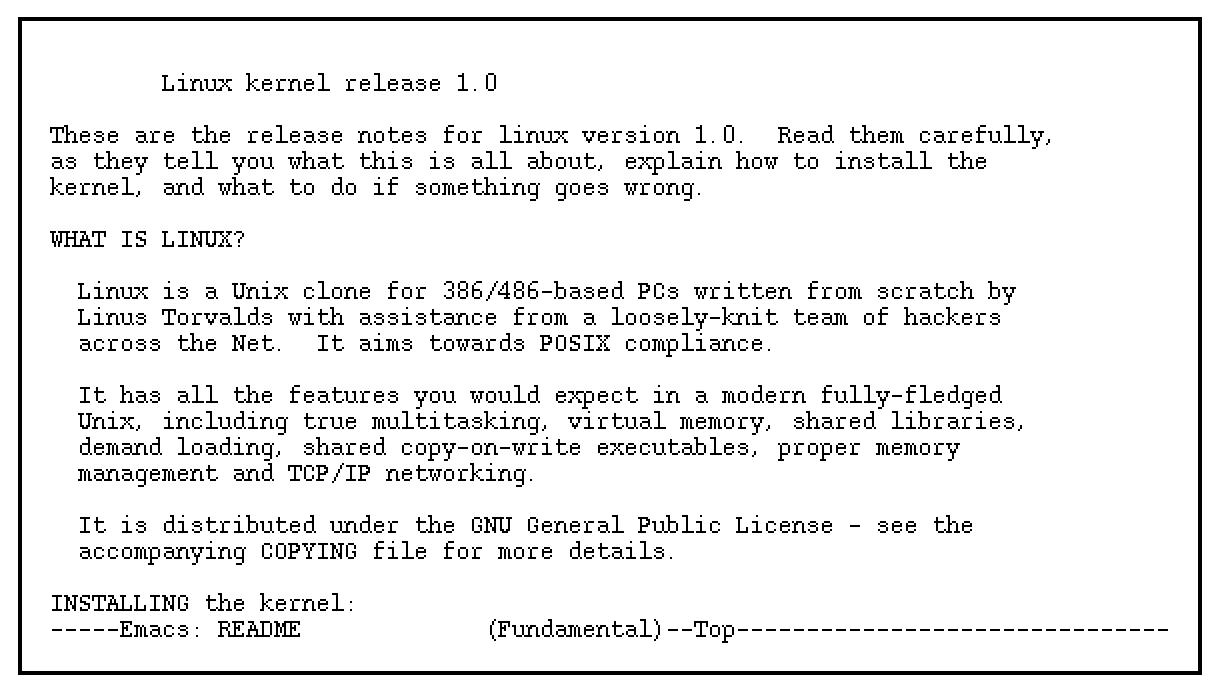
\epsfig{file=ps-files/screen-shot-1.ps, width=5in}
\end{center}
\caption{Emacs was just started with {\tt emacs README}}
\end{figure}

In my mode line, you see ``Top''. It might be ``All'' instead, and
there may be other minor differences. (Many people have the current
time displayed in the mode line.) The line immediately below the mode
line is called the {\bf minibuffer}, or sometimes the {\bf echo area}.
Emacs uses the minibuffer to flash messages at you, and occasionally
uses it to read input from you, when necessary.  In fact, right now
Emacs is telling you ``{\tt For information about the GNU Project and
  its goals, type C-h C-p.}'' Ignore it for now; we won't be making
much use of the minibuffer for a while.

Before you actually change any of the text in the file, you need to
learn how to move around.  The cursor should be at the beginning of
the file, in the upper-left corner of the screen.  To move forward,
type {\tt C-f} (that is, hold down the \key{Control} key while you
press ``f'', for ``forward'').  It will move you forward a character
at a time, and if you hold both keys down, your system's automatic
key-repeat should take effect in a half-second or so.  Notice how when
you get to the end of the line, the cursor automatically moves to the
next line.  {\tt C-b} (for ``backward'') has the opposite behavior.  And,
while we're at it, {\tt C-n} and {\tt C-p} take you to the next and
previous lines, respectively.\footnote{In case you hadn't noticed yet,
  many of Emacs's movement commands consist of combining
  \key{Control} with a single mnemonic letter.}

Using the control keys is usually the quickest way of moving around
when you're editing. The goal of {\tt Emacs} is to keep your hands
over the alpha-numeric keys of the keyboard, where most of your work
gets done. However, if you want to, the arrow keys should also work.

\xwarn In fact, when you're using X, you should be able to position
the mouse pointer and click with the left button to move the cursor
where you want. However, this is very slow---you have to move your
hand all the way to your mouse! Most people who use Emacs primarily
use the keyboard for getting around.

Use {\tt C-p} and {\tt C-b} to get all the way back to the upper-left
corner. Now keep {\tt C-b} held a little longer.  You should
hear an annoying bell sound, and see the message ``{\tt Beginning of
  buffer}'' appear in the minibuffer.  At this point you
might wonder, ``But what is a buffer?''

When Emacs works on a file, it doesn't actually work on the file
itself.  Instead, it copies the contents of the file into a special
Emacs work area called a {\bf buffer}, where you can modify it to your
heart's content.  When you are done working, you tell Emacs to save
the buffer---in other words, to write the buffer's contents into the
corresponding file.  Until you do this, the file remains unchanged,
and the buffer's contents exist only inside of Emacs.

        With that in mind, prepare to insert your first character into
the buffer.  Until now, everything we have done has been
``non-destructive'', so this is a big moment.  You can choose any
character you like, but if you want to do this in style, I suggest
using a nice, solid, capital ``X''.  As you type it, take a look at
the beginning of the mode line at the bottom of the screen.  When you
change the buffer so that its contents are no longer the same as those
of the file on disk, Emacs displays two asterisks at the beginning of
the mode line, to let you know that the buffer has been modified:

\begin{screen}
   \begin{verbatim}
--**-Emacs: some_file.txt           (Fundamental)--Top------------------------
\end{verbatim}
\end{screen}

        These two asterisks are displayed as soon as you modify the
buffer, and remain visible until you save the buffer.  You can save
the buffer multiple times during an editing session---the command to
do so is just {\tt C-x~C-s} (hold down \key{Control} and hit ``x''
and ``s'' while it's down\ldots okay, so you probably already figured
that out!).  It's deliberately easy to type, because saving your
buffers is something best done early and often.

I'm going to list a few more commands now, along with the ones you've
learned already, and you can practice them however you like.  I'd
suggest becoming familiar with them before going any further:

\begin{tabular}{ll}
{\bf {\tt C-f}}       & Move forward one character. \\
{\bf {\tt C-b}}       & Move backward one character. \\
{\bf {\tt C-n}}       & Go to next line. \\
{\bf {\tt C-p}}       & Go to previous line. \\
{\bf {\tt C-a}}       & Go to beginning of line. \\
{\bf {\tt C-e}}       & Go to end of line. \\
{\bf {\tt C-v}}       & Go to next page/screenful of text. \\
{\bf {\tt C-l}}       & Redraw the screen, with current line in center. \\
{\bf {\tt C-d}}       & Delete this character (practice this one). \\
{\bf {\tt C-k}}       & Delete text from here to end of line. \\
{\bf {\tt C-x C-s}}   & Save the buffer in its corresponding file. \\
\key{Backspace}       & Delete preceding character (the one you just typed). \\
\end{tabular}

\section{Getting Started Quickly in X}

\xwarn If all you're interesting in is editing a few files quickly, an
X user doesn't have to go much further beyond the menus at the top of
the screen: 

\begin{center}
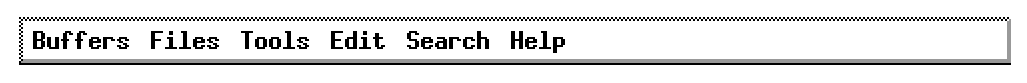
\epsfig{file=ps-files/screen-shot-2.ps,width=\textwidth}
\end{center}

These menus are not available in text mode.

When you first start Emacs, there will be four menus at the top of the
screen: {\sf Buffers}, {\sf File}, {\sf Edit}, and {\sf Help}. To use
a menu, simply move the mouse pointer over the name (like {\sf File},
click and hold down on the left button. Then, move the pointer to the
action you want and release the mouse button. If you change your mind,
move the mouse pointer away from the menu and release the button.

The {\sf Buffers} menu lists the different files you've been editing
in this incarnation of Emacs.The {\sf File} menu shows a bunch of
commands for loading and saving files---many of them will be described
later. The {\sf Edit} menu displays some commands for editing one
buffer, and the {\sf Help} menu should hopefully give on-line
documentation.

You'll notice keyboard equivalents are listed next to the choices in
the menu. Since, in the long run, they'll be quicker, you might want
to learn them. Also, for better or for worse, most of Emacs's
functionality is {\em only\/} available through the keyboard---you
might want to read the rest of this chapter.

\section{Editing Many Files at Once}

Emacs can work on more than one file at a time.  In fact, the only
limit on how many buffers your Emacs can contain is the actual amount
of memory available on the machine. The command to bring a new file
into an Emacs buffer is {\tt C-x~C-f}.  When you type it, you will be
prompted for a filename in the minibuffer:

\begin{screen}
   \begin{verbatim}
Find file: ~/
   \end{verbatim}
\end{screen}

        The syntax here is the same one used to specify files from the
shell prompt; slashes represent subdirectories, \verb+~+means your
home directory.  You also get {\bf filename completion}, meaning
that if you've typed enough of a filename at the prompt to identify
the file uniquely, you can just hit \key{Tab} to complete it (or to
show possible completions, if there are more than one).  \key{Space}
also has a role in filename completion in the minibuffer, similar to
\key{Tab}, but I'll let you experiment to find out how the two differ.
% translation: I know they're different, but I can never figure out how!
Once you have the full filename in the minibuffer, hit \key{Return},
and Emacs will bring up a buffer displaying that file.  In Emacs, this
process is known as {\bf finding} a file.  Go ahead and find some
other unimportant text file now, and bring it into Emacs (do this from
our original buffer {\tt some\_file.txt}).  Now you have a new buffer;
I'll pretend it's called {\tt another\_file.txt}, since I can't see
your mode line.

        Your original buffer seems to have disappeared---you're
probably wondering where it went.  It's still inside Emacs, and you
can switch back to it with {\tt C-x~b}.  When you type this, you will
see that the minibuffer prompts you for a buffer to switch to, and it
names a default.  The default is the buffer you'd get if you just hit
\key{Return} at the prompt, without typing a buffer name.  The default
buffer to switch to is always the one most recently left, so that when
you are doing a lot of work between two buffers, {\tt C-x~b} always
defaults to the ``other'' buffer (which saves you from having to type
the buffer name).  Even if the default buffer is the one you want,
however, you should try typing in its name anyway.

        Notice that you get the same sort of completion you got when
finding a file: hitting \key{Tab} completes as much of a buffer name
as it can, and so on.  Whenever you are being prompted for something
in the minibuffer, it's a good idea to see if Emacs is doing
completion.  Taking advantage of completion whenever it's offered will
save you a lot of typing.  Emacs usually does completion when you are
choosing one item out of some predefined list.

Everything you learned about moving around and editing text in the
first buffer applies to the new one.  Go ahead and change some text in
the new buffer, but don't save it (i.e.\ don't type {\tt C-x~C-s}).
Let's assume that you want to discard your changes without saving them
in the file.  The command for that is {\tt C-x~k}, which ``kills'' the
buffer.  Type it now.  First you will be asked which buffer to kill,
but the default is the current buffer, and that's almost always the
one you want to kill, so just hit \key{Return}.  Then you will be
asked if you {\em really\/} want to kill the buffer---Emacs always
checks before killing a buffer that has unsaved changes in it.  Just
type ``yes'' and hit \key{Return}, if you want to kill it.

        Go ahead and practice loading in files, modifying them, saving
them, and killing their buffers.  Make sure you don't modify any
important system files in a way that will cause trouble\footnote{If
you are not the ``root'' user on the machine, you shouldn't be able to
hurt the system anyway, but be careful just the same.}, of course, but
do try to have at least five buffers open at once, so you can get the
hang of switching between them.

\section{Ending an Editing Session}

When you are done with your work in Emacs, make sure that all buffers
are saved that should be saved, and exit Emacs with {\tt C-x~C-c}.
Sometimes {\tt C-x~C-c} will ask you a question or two in the
minibuffer before it lets you leave---don't be alarmed, just answer
them in the obvious ways.  If you think that you might be returning to
Emacs later, don't use {\tt C-x~C-c} at all; use {\tt C-z}, which will
suspend Emacs.  You can return to it with the shell command ``{\tt
  fg}'' later. This is more efficient than stopping and starting Emacs
multiple times, especially if you have edit the same files again
later.

\xwarn Under X, hitting {\tt C-z} will merely iconize the window. See
the section on iconization in Chapter~\ref{x-chapter}. This gives you
two ways of iconizing Emacs---the normal way your window manager
offers, and {\tt C-z}. Remember, when you iconize, a simply {\tt fg}
won't bring the window back---you'll have to use your window manager.

\section{The Meta Key}

You've already learned about one ``modifier key'' in Emacs, the
\key{Control} key.  There is a second one, called the {\bf Meta}
key, which is used almost as frequently.  However, not all keyboards
have their Meta key in the same place, and some don't have one at all.
The first thing you need to do is find where your Meta key is located.
Chances are, your keyboard's \key{Alt} keys are also Meta keys, if
you are using an IBM PC or other another keyboard that has an
\key{Alt} key.

        The way to test this is to hold down a key that you think
might be a Meta key and type ``x''.  If you see a little prompt appear
in the minibuffer (like this: {\tt M-x}) then you've found it.  To get
rid of the prompt and go back to your Emacs buffer, type {\tt C-g}.

If you didn't get a prompt, then there is still one solution.  You can
use the \key{Escape} key as a Meta key.  But instead of holding it
down while you type the next letter, you have to tap it and release it
quickly, and {\em then\/} type the letter.  This method will work
whether or not you have a real Meta key, so it's the safest way to go.
Try tapping \key{Escape} and then typing ``x'' now.  You should get
that tiny prompt again.  Just use {\tt C-g} to make it go away.  {\tt
  C-g}\index{emacs!interrupting} is the general way in Emacs to quit
out of something you don't mean to be in.  It usually beeps annoyingly
at you to let you know that you have interrupted something, but that's
fine, since that's what you intended to do if you typed {\tt
  C-g}\/!\footnote{Occasionally, even one {\tt C-g} isn't enough to
  persuade Emacs that you really wanted to interrupt what you're
  doing. Just keep at it, and Emacs will usually return to a saner
  mode.}

         The notation {\tt M-x} is analogous to {\tt C-x} (substitute
any character for ``{\tt x}'').  If you have found a real Meta key,
use that, otherwise just use the \key{Escape} key.  I will simply
write {\tt M-x} and you'll have to use your own Meta key.

\section{Cutting, Pasting, Killing and Yanking}
        
Emacs, like any good editor, allows you to cut and paste blocks of
text.  In order to do this, you need a way to define the start and end
of the block.  In Emacs, you do this by setting two locations in the
buffer, known as {\bf mark}\index{emacs!mark} and {\bf
  point}\index{emacs!point}.  To set the mark, go to the place you
want your block to begin and type {\tt C-SPC} (``{\tt SPC}'' means
\key{Space}, of course).  You should see the message ``Mark set''
appear in the minibuffer.\footnote{On some terminals, {\tt C-SPC} doesn't
  work.  For these machines, you must use {\tt C-@}.} The mark has now
been set at that place.  There will be no special highlighting
indicating that fact, but you know where you put it, and that's all
that matters.

What about {\bf point}?  Well, it turns out that you've been setting
point every time you move the cursor, because ``point'' just refers to
your current location in the buffer.  In formal terms, point is the
spot where text would be inserted if you were to type something.  By
setting the mark, and then moving to the end of the block of text, you
have actually defined a block of text.  This block is known as the
{\bf region}\index{emacs!region}.  The region always means the area
between mark and point.

Merely defining the region does not make it available for pasting.
You have to tell Emacs to copy it in order to be able to paste it.  To
copy the region, make sure that mark and point are set correctly, and
type {\tt M-w}.  It has now been recorded by Emacs.  In order to paste
it somewhere else, just go there and type {\tt C-y}.  This is known as
{\bf yanking}\index{emacs!yanking} the text into the buffer.

If you want to actually move the text of the region to somewhere else,
type {\tt C-w} instead of {\tt M-w}.  This will {\bf
  kill}\index{emacs!kill} the region---all the text inside it will
disappear.  In fact, it has been saved in the same way as if you had
used {\tt M-w}.  You can yank it back out with {\tt C-y}, as always.
The place Emacs saves all this text is known as the {\bf kill-ring}.
Some editors call it the ``clipboard'' or the ``paste buffer''.

        There's another way to do cutting and pasting: whenever you
use {\tt C-k} to kill to the end of a line, the killed text is saved
in the kill-ring.  If you kill more than one line in a row, they are
all saved in the kill-ring together, so that the next yank will paste
in all the lines at once.  Because of this feature, it is often faster
to use repeated {\tt C-k}'s to kill some text than it is to explicitly
set mark and point and use {\tt C-w}.  However, either way will work.
It's really a matter of personal preference how you do it.

\section{Searching and Replacing}

There are several ways to search for text in Emacs.  Many of them are
rather complex, and not worth going into here.  The easiest and most
entertaining way is to use {\bf isearch}\bindex{emacs!searching}.
``Isearch'' stands for ``incremental search''.  Suppose you want to
search for the string ``gadfly'' in the following buffer:

\begin{quote}
   \begin{tt}
        I was growing afraid that we would run out of gasoline, when
my passenger exclaimed ``Gadzooks!  There's a gadfly in here!''.
   \end{tt}
\end{quote}

You would move to the beginning of the buffer, or at least to some
point that you know is before the first occurence of the goal word,
``gadfly'', and type {\tt C-s}.  That puts you in isearch mode.  Now
start typing the word you are searching for, ``gadfly''.  But as soon
as you type the ``g'', you see that Emacs has jumped you to the first
occurence of ``g'' in the buffer.  If the above quote is the entire
contents of the buffer, then that would be the first ``g'' of the word
``growing''.  Now type the ``a'' of ``gadfly'', and Emacs leaps over
to ``gasoline'', which contains the first occurence of a ``ga''.  The
``d'' gets you to gadzooks, and finally, ``f'' gets you to ``gadfly'',
without your having had to type the entire word.

        What you are doing in an isearch is defining a string to
search for.  Each time you add a character to the end of the string,
the number of matches is reduced, until eventually you have entered
enough to define the string uniquely.  Once you have found the match
you are looking for, you can exit the search with \key{Return} or any
of the normal movement commands.  If you think the string you're
looking for is behind you in the buffer, then you should use {\tt
C-r}, which does an isearch backwards.

        If you encounter a match, but it's not the one you were
looking for, then hit {\tt C-s} again while still in the search.  This
will move you forward to the next complete match, each time you hit
it.  If there is no next match, it will say that the search failed,
but if you press {\tt C-s} again at that point, the search will wrap
around from the beginning of the buffer.  The reverse holds true for
{\tt C-r} --- it wraps around the end of the buffer.

        Try bringing up a buffer of plain English text and doing and
isearch for the string ``{\tt the}''.  First you'd type in as much as
you wanted, then use repeated {\tt C-s}'s to go to all instances of
it.  Notice that it will match words like ``{\tt them}'' as well,
since that also contains the substring ``{\tt the}''.  To search only
for ``{\tt the}'', you'd have to do add a space to the end of your
search string.  You can add new characters to the string at any point
in the search, even after you've hit {\tt C-s} repeatedly to find the
next matches.  You can also use \key{Backspace} or \key{Delete} to
remove characters from the search string at any point in the search,
and hitting \key{Return} exits the search, leaving you at the last
match.

        Emacs also allows you to replace all instances of a string
with some new string---this is known as {\bf query-replace}.  To
invoke it, type {\tt query-replace} and hit \key{Return}.
Completion is done on the command name, so once you have typed
``query-re'', you can just hit \key{Tab} to finish it.  Say you wish
to replace all instances of ``gadfly'' with ``housefly''.  At the
``{\tt Query replace:\, }'' prompt, type ``gadfly'', and hit
\key{Return}.  Then you will be prompted again, and you should enter
``housefly''.  Emacs will then step through the buffer, stopping at
every instance of the word ``gadfly'', and asking if you want to
replace it.  Just hit ``{\tt y}'' or ``{\tt n}'' at each instance, for
``Yes'' or ``No'', until it finishes.  If this doesn't make sense as
you read it, then try it out.
\eindex{emacs!searching}

\section{What's Really Going On Here?}

        Actually, all these {\bf keybindings} you have been learning
are shortcuts to Emacs functions.  For example, {\tt C-p} is a short
way of telling Emacs to execute the internal function {\tt
previous-line}.  However, all these internal functions can be called
by name, using {\tt M-x}.  If you forgot that {\tt previous-line} is
bound to {\tt C-p}, you could just type {\tt M-x previous-line}
\key{Return}, and it would move you up one line.  Try this now, to
understand how {\tt M-x previous-line} and {\tt C-p} are really the
same thing.

        The designer of Emacs started from the ground up, first
defining a whole lot of internal functions, and then giving
keybindings to the most commonly-used ones.  Sometimes it's easier
just to call a function explicitly with {\tt M-x} than to remember
what key it's bound to.  The function {\tt query-replace}, for
example, is bound to {\tt M-\%} in some versions of Emacs.  But who
can remember such an odd keybinding?  Unless you use query-replace
extremely often, it's easier just to call it with {\tt M-x}.

        Most of the keys you type are letters, meant to be inserted
into the text of the buffer.  So each of those keys is {\bf bound} to
the function {\tt self-insert-command}, which does nothing but insert
that letter into the buffer.  Combinations that use the \key{Control}
key with a letter are generally bound to functions that do other
things, like moving you around.  For example, {\tt C-v} is bound to a
function called {\tt scroll-up}, which scrolls the buffer up by one
screenful (meaning that your position in the buffer moves {\em
down\/}, of course).

        If you ever actually wanted to insert a Control character into
the buffer, then, how would you do it?  After all, the Control
characters are {\tt ASCII} characters, although rarely used, and you
might want them in a file.  There is a way to prevent Control
characters from being interpreted as commands by Emacs.  The key {\tt
C-q}\footnote{We call {\tt C-q} a ``key'', even though it is produced
by holding down \key{Control} and pressing ``q'', because it is a
single {\tt ASCII} character.} is bound to a special function named
{\tt quoted-insert}.  All {\tt quoted-insert} does is read the next
key and insert it literally into the buffer, without trying to
interpret it as a command.  This is how you can put Control characters
into your files using Emacs.  Naturally, the way to insert a C-q is to
press {\tt C-q} twice!

Emacs also has many functions that are not bound to any key.  For
example, if you're typing a long message, you don't want to have to
hit return at the end of every line.  You can have Emacs do it for you
(you can have Emacs do anything for you)---the command to do so is
called {\tt auto-fill-mode}, but it's not bound to any keys by
default.  In order to invoke this command, you would type ``{\tt
  M-x~auto-fill-mode}''.  ``{\bf\tt M-x}'' is the key used to call
functions by name.  You could even use it to call functions like {\tt
  next-line} and {\tt previous-line}, but that would be very
inefficient, since they are already bound to {\tt C-n} and {\tt C-p}!

        By the way, if you look at your mode line after invoking {\tt
auto-fill-mode}, you will notice that the word ``Fill'' has been added
to the right side.  As long as it's there, Emacs will fill (wrap) text
automatically.  You can turn it off by typing ``{\tt
M-x~auto-fill-mode}'' again---it's a toggle command.

        The inconvenience of typing long function names in the
minibuffer is lessened because Emacs does completion on function names
the same way it does on file names.  Therefore, you should rarely find
yourself typing in the whole function name, letter by letter.  If
you're not sure whether or not you can use completion, just hit
\key{Tab}.  It can't hurt: the worst thing that will happen is that
you'll just get a tab character, and if you're lucky, it'll turn out
that you can use completion.

\section{Asking Emacs for Help}

        Emacs has extensive help facilities---so extensive, in fact,
that we can only touch on them here.  The most basic help features are
accessed by typing {\tt C-h} and then a single letter.  For example,
{\tt C-h~k} gets help on a key (it prompts you to type a key, then
tells you what that key does).  {\tt C-h~t} brings up a short Emacs
tutorial.  Most importantly, {\tt C-h~C-h~C-h} gets you help on help,
to tell you what's available once you have typed {\tt C-h} the first
time.  If you know the name of an Emacs function ({\tt save-buffer},
for example), but can't remember what key sequence invokes it, then
use {\tt C-h~w}, for ``{\tt where-is}'', and type in the name of the
function.  Or, if you want to know what a function does in detail, use
{\tt C-h~f}, which prompts for a function name.

        Remember, since Emacs does completion on function names, you
don't really have to be sure what a function is called to ask for help
on it.  If you think you can guess the word it might start with, type
that and hit \key{Tab} to see if it completes to anything.  If not,
back up and try something else.  The same goes for file names: even if
you can't remember quite what you named some file that you haven't
accessed for three months, you can guess and use completion to find
out if you're right.  Get used to using completion as means of asking
questions, not just as a way of saving keystrokes.

        There are other characters you can type after {\tt C-h}, and
each one gets you help in a different way.  The ones you will use most
often are {\tt C-h~k}, {\tt C-h~w}, and {\tt C-h~f}.  Once you are
more familiar with Emacs, another one to try is {\tt C-h~a}, which
prompts you for a string and then tells you about all the functions
who have that string as part of their name (the ``a'' means for
``apropos'', or ``about'').

        Another source of information is the {\bf Info} documentation
reader.  Info is too complex a subject to go into here, but if you are
interested in exploring it on your own, type {\tt C-h~i} and read the
paragraph at the top of the screen.  It will tell you how get more
help.

\section{Specializing Buffers: Modes}\label{emacs-mail-mode}

Emacs buffers have {\bf modes} associated with them\footnote{To make
  matters worse, there are ``Major Modes'' and ``Minor Modes'', but
  you don't need to know about that right now.}.  The reason for this
is that your needs when writing a mail message are very different from
your needs when, say, writing a program.  Rather than try to come up
with an editor that would meet every single need all the time (which
would be impossible), the designer of Emacs\footnote{Richard
  Stallman\index{Stallman, Richard}, also sometimes referred to as
  ``{\tt rms}'', because that's his login name.} chose to have Emacs
behave differently depending on what you are doing in each individual
buffer.  Thus, buffers have modes, each one designed for some specific
activity.  The main features that distinguish one mode from another
are the keybindings, but there can be other differences as well.

        The most basic mode is {\tt fundamental} mode, which doesn't
really have any special commands at all.  In fact, here's what Emacs
has to say about Fundamental Mode:

\begin{tt}
   \begin{verbatim}
Fundamental Mode:

Major mode not specialized for anything in particular.
Other major modes are defined by comparison with this one.
\end{verbatim}
\end{tt}

        I got that information like this: I typed {\tt C-x~b}, which
is {\tt switch-to-buffer}, and entered ``foo'' when it prompted me for
a buffer name to switch to.  Since there was previously no buffer
named ``{\tt foo}'', Emacs created one and switched me to it.  It was
in {\tt fundamental-mode} by default, but it it hadn't been, I could
have typed ``{\tt M-x~fundamental-mode}'' to make it so.  All mode
names have a command called {\tt <modename>-mode} which puts the
current buffer into that mode.  Then, to find out more information
about that major mode, I typed {\tt C-h~m}, which gets you help on the
current major mode of the buffer you're in.

        There's a slightly more useful mode called {\tt text-mode},
which has the special commands {\tt M-S}, for {\tt center-paragraph},
and {\tt M-s}, which invokes {\tt center-line}.  {\tt M-S}, by the
way, means exactly what you think it does: hold down both the
\key{Meta} and the \key{Shift} key, and press ``S''.

        Don't just take my word for this---go make a new buffer, put
it into {\tt text-mode}, and type {\tt C-h~m}.  You may not understand
everything Emacs tells you when you do that, but you should be able to
get some useful information out of it.

        Here is an introduction to some of the more commonly used
modes.  If you use them, make sure that you type {\tt C-h~m} sometime
in each one, to find out more about each mode.

\section{Programming Modes}

\subsection{C Mode}

        If you use Emacs for programming in the C language\index{C}, you can
get it to do all the indentation for you automatically.  Files whose
names end in ``{\tt .c} '' or ``{\tt .h}'' are automatically brought
up in {\tt c-mode}.  This means that certain special editing commands,
useful for writing C-programs, are available.  In C-mode, \key{Tab} is
bound to {\tt c-indent-command}.  This means that hitting the
\key{Tab} key does not actually insert a tab character.  Instead, if
you hit \key{Tab} anywhere on a line, Emacs automatically indents
that line correctly for its location in the program.  This implies
that Emacs knows something about C syntax, which it does (although
nothing about semantics---it cannot insure that your program has no
errors!)

        In order to do this, it assumes that the previous lines are
indented correctly.  That means that if the preceding line is missing
a parenthesis, semicolon, curly brace, or whatever, Emacs will indent
the current line in a funny way.  When you see it do that, you will
know to look for a punctuation mistake on the line above.
        
        You can use this feature to check that you have punctuated
your programs correctly---instead of reading through the entire
program looking for problems, just start indenting lines from the top
down with \key{Tab}, and when something indents oddly, check the
lines just before it.  In other words, let Emacs do the work for you!


\subsection{Scheme Mode}
% kff: larry, I include this because people at our school are using
% this document too, and they need scheme for classes.  Also, with the
% availability of SCM, scheme seems to be gaining some popularity
% among linuxers.  Feel free to remove this subsection if you think
% it's not necessary, though.  Is there a way to do a conditional
% include in LaTeX?  Would you like me to make this multifile and use
% \include and \includeonly ?

This is a major mode that won't do you any good unless you have a
compiler or an interpreter for the Scheme programming language on your
system.  Having one is not as normal as having, say, a C compiler, but
it's becoming more and more common, so I'll cover it too.  Much of
what is true for Scheme\index{scheme} mode is true for Lisp mode as
well, if you prefer to write in Lisp\index{lisp}.

Well, to make matters painful, Emacs comes with two different Scheme
modes, because people couldn't decide how they wanted it to work.  The
one I'm describing is called {\tt cmuscheme}\ttindex{cmuscheme}, and
later on, in the section on customizing Emacs, I'll talk about how
there can be two different Scheme modes and what to do about it.  For
now, don't worry about it if things in your Emacs don't quite match up
to what I say here.  A customizable editor means an unpredictable
editor, and there's no way around that!

% todo: this won't work unless Emacs knows where to find the scheme
% interpreter.  Should we talk about that?  Yes, in the section on
% elisp, mention setting scheme-program-name.

        You can run an interactive Scheme process in Emacs, with the
command {\tt M-x run-scheme}.  This creates a buffer named ``{\tt
*scheme*}'', which has the usual Scheme prompt in it.  You can type in
Scheme expressions at the prompt, hit \key{Return}, and Scheme will
evaluate them and display the answer.  Thus, in order to interact with
the Scheme process, you could just type all your function definitions
and applications in at the prompt.  Chances are you have
previously-written Scheme source code in a file somewhere, and it
would be easier to do your work in that file and send the definitions
over to the Scheme process buffer as necessary.

        If that source file ends in ``{\tt .ss}'' or ``{\tt .scm}'',
it will automatically be brought up in {\bf Scheme mode} when you find
it with {\tt C-x~C-f}.  If for some reason, it doesn't come up in
Scheme mode, you can do it by hand with {\tt M-x scheme-mode}.  This
{\tt scheme-mode} is not the same thing as the buffer running the
Scheme process; rather, the source code buffer's being in {\tt
scheme-mode} means that it has special commands for communicating with
the process buffer.

        If you put yourself inside a function definition in the Scheme
source code buffer and type {\tt C-c~C-e}, then that definition will
be ``sent'' to the process buffer --- exactly as if you had typed it
in yourself.  {\tt C-c~M-e} sends the definition and then brings you
to the process buffer to do some interactive work.  {\tt C-c~C-l}
loads a file of Scheme code (this one works from either the process
buffer or the source code buffer).  And like other programming
language modes, hitting \key{Tab} anywhere on a line of code correctly
indents that line.

        If you're at the prompt in the process buffer, you can use
{\tt M-p} and {\tt M-n} to move through your previous commands (also
known as the {\bf input history}).  So if you are debugging the
function {\tt `rotate'}, and have already applied it to arguments in
the process buffer, like so:

\begin{screen}
   \begin{tt}
{\tt > (rotate '(a b c d e))}
   \end{tt}
\end{screen}

        then you can get that command back by typing {\tt M-p} at the
prompt later on.  There should be no need to retype long expressions
at the Scheme prompt --- get in the habit of using the input history
and you'll save a lot of time.

        Emacs knows about quite a few programming languages: C, C++,
Lisp, and Scheme are just some.  Generally, it knows how to indent
them in intuitive ways.

\subsection{Mail Mode}

        You can also edit and send mail\index{mail} in Emacs.  To enter a mail
buffer, type {\tt C-x~m}.  You need to fill in the {\tt To:} and {\tt
Subject:} fields, and then use C-n to get down below the separator
line into the body of the message (which is empty when you first start
out).  Don't change or delete the separator line, or else Emacs will
not be able to send your mail---it uses that line to distinguish
the mail's headers, which tell it where to send the mail, from the
actual contents of the message.

        You can type whatever you want below the separator line.  When
you are ready to send the message, just type {\tt C-c~C-c}, and Emacs
will send it and then make the mail buffer go away.

\section{Being Even More Efficient}

        Experienced Emacs users are fanatical about efficiency.  In
fact, they will often end up wasting a lot of time searching for ways
to be more efficient!  While I don't want that to happen to you, there
are some easy things you can do to become a better Emacs user.
Sometimes experienced users make novices feel silly for not knowing
all these tricks---for some reason, people become religious about
using Emacs ``correctly''.  I'd condemn that sort of elitism more if I
weren't about to be guilty of it myself.  Here we go:

        When you're moving around, use the fastest means available.
You know that {\tt C-f} is {\tt forward-char}---can you guess that
{\tt M-f} is {\tt forward-word}?  {\tt C-b} is {\tt backward-char}.
Guess what {\tt M-b} does?  That's not all, though: you can move
forward a sentence at a time with {\tt M-e}, as long as you write
your sentences so that there are always two spaces following the final
period (otherwise Emacs can't tell where one sentence ends and the
next one begins).  {\tt M-a} is {\tt backward-sentence}.

        If you find yourself using repeated {\tt C-f}'s to get to the
end of the line, be ashamed, and make sure that you use {\tt C-e}
instead, and {\tt C-a} to go to the beginning of the line.  If you use
many {\tt C-n}'s to move down screenfuls of text, be very ashamed, and
use {\tt C-v} forever after.  If you are using repeated {\tt C-p}'s to
move up screenfuls, be embarrassed to show your face, and use {\tt
M-v} instead.

        If you are nearing the end of a line and you realize that
there's a mispelling or a word left out somewhere earlier in the line,
{\em don't} use \key{Backspace} or \key{Delete} to get back to that
spot.  That would require retyping whole portions of perfectly good
text.  Instead, use combinations of {\tt M-b}, {\tt C-b}, and {\tt
C-f} to move to the precise location of the error, fix it, and then
use {\tt C-e} to move to the end of the line again.

        When you have to type in a filename, don't ever type in the
whole name.  Just type in enough of it to identify it uniquely, and
let Emacs's completion finish the job by hitting \key{Tab} or
\key{Space}.  Why waste keystrokes when you can waste CPU cycles
instead?

        If you are typing some kind of plain text, and somehow your
auto-filling (or auto-wrapping) has gotten screwed up, use {\tt M-q},
which is {\tt fill-paragraph} in common text modes.  This will
``adjust'' the paragraph you're in as if it had been wrapped line by
line, but without your having to go mess around with it by hand.  {\tt
M-q} will work from inside the paragraph, or from its very beginning
or end.

Sometimes it's helpful to use {\tt C-x~u}, ({\bf undo}), which will
try to ``undo'' the last change(s) you made.  Emacs will guess at how
much to undo; usually it guesses very intelligently.  Calling it
repeatedly will undo more and more, until Emacs can no longer remember
what changes were made.

\section{Customizing Emacs}

% Dang it, I *am* going to talk about elisp.  They're gonna become
% pros if it kills them!

% todo: need to talk about xscheme vs. cmuscheme and what load-path,
% .emacs, default.el and the distribution lisp dir have to do with it,
% the elisp info manual, setting keys, binding variables.  Defining
% functions?  Should we cover things like `let', or tell people to go
% learn Lisp first? 

        Emacs is {\em so} big, and {\em so} complex, that it actually
has its own programming language!  I'm not kidding: to really
customize Emacs to suit your needs, you have to write programs in this
language.  It's called Emacs Lisp, and it's a dialect of Lisp, so if
you have previous experience in Lisp, it will seem quite friendly.  If
not, don't worry: I'm not going to go into a great deal of depth,
because it's definitely best learned by doing.  To really learn about
programming Emacs, you should consult the Info pages on Emacs Lisp,
and read a lot of Emacs Lisp source code.

Most of Emacs's functionality is defined in files of Emacs
Lisp\footnote{Sometimes unofficially called ``Elisp''.} code.  Most of
these files are distributed with Emacs and collectively are known as
the ``Emacs Lisp library''.  This library's location depends on how
Emacs was installed on your system --- common locations are {\tt
  /usr/lib/emacs/lisp}, {\tt /usr/lib/emacs/19.19/lisp/}, etc.  The
``{\tt 19.19}'' is the version number of Emacs, and might be different
on your system.

        You don't need to poke around your filesystem looking for the
lisp library, because Emacs has the information stored internally, in
a variable called {\tt\bf load-path}.  To find out the value of this
variable, it is necessary to {\bf evaluate} it; that is, to have
Emacs's lisp interpreter get its value.  There is a special mode for
evaluating Lisp expressions in Emacs, called {\tt\bf
lisp-interaction-mode}.  Usually, there is a buffer called ``{\tt
*scratch*}'' that is already in this mode.  If you can't find one,
create a new buffer of any name, and type {\tt M-x
lisp-interaction-mode} inside it.

        Now you have a workspace for interacting with the Emacs Lisp
interpreter.  Type this:

\begin{screen}
   \begin{tt}
load-path
   \end{tt}
\end{screen}

        and then press {\tt C-j} at the end of it.  In
lisp-interaction-mode, {\tt C-j} is bound to {\tt
eval-print-last-sexp}.  An ``{\tt sexp}'' is an ``{\tt\bf
s-expression}'', which means a balanced group of parentheses,
including none.  Well, that's simplifying it a little, but you'll get
a feel for what they are as you work with Emacs Lisp.  Anyway,
evaluating {\tt load-path} should get you something like this:

\begin{screen}
   \begin{tt}
load-path\key{C-j} \\
("/usr/lib/emacs/site-lisp/vm-5.35" "/home/kfogel/elithp" \\
 "/usr/lib/emacs/site-lisp" "/usr/lib/emacs/19.19/lisp")
   \end{tt}
\end{screen}

        It won't look the same on every system, of course, since it is
dependant on how Emacs was installed.  The above example comes from my
386 PC running Linux.  As the above indicates, {\tt load-path} is a
list of strings.  Each string names a directory that might contain
Emacs Lisp files.  When Emacs needs to load a file of Lisp code, it
goes looking for it in each of these directories, in order.  If a
directory is named but does not actually exist on the filesystem,
Emacs just ignores it.

        When Emacs starts up, it automatically tries to load the file
{\tt .emacs} in your home directory.  Therefore, if you want to make
personal customizations to Emacs, you should put them in {\tt .emacs}.
The most common customizations are keybindings, so here's how to do
them:

\begin{screen}
   \begin{tt}
(global-set-key "\verb+\+C-cl" 'goto-line)
   \end{tt}
\end{screen}

        {\tt global-set-key} is a function of two arguments: the key
to be bound, and the function to bind it to.  The word ``{\tt
global}'' means that this keybinding will be in effect in all major
modes (there is another function, {\tt local-set-key}, that binds a
key in a single buffer).  Above, I have bound {\tt C-c~l} to the
function {\tt goto-line}.  The key is described using a string.  The
special syntax ``{\tt \verb+\+C-<char>}'' means the \key{Control}
key held down while the key {\tt <char>} is pressed.  Likewise, ``{\tt
\verb+\+M-<char>}'' indicates the \key{Meta} key.

        All very well, but how did I know that the function's name was
``{\tt goto-line}''?  I may know that I want to bind {\tt C-c~l} to
some function that prompts for a line number and then moves the cursor
to that line, but how did I find out that function's name?

        This is where Emacs's online help facilities come in.  Once you
have decided what kind of function you are looking for, you can use
Emacs to track down its exact name.  Here's one quick and dirty way to
do it: since Emacs gives completion on function names, just type {\tt
C-h~f} (which is {\tt describe-function}, remember), and then hit
\key{Tab} without typing anything.  This asks Emacs to do completion
on the empty string --- in other words, the completion will match
every single function!  It may take a moment to build the completion
list, since Emacs has so many internal functions, but it will display
as much of it as fits on the screen when it's ready.

        At that point, hit {\tt C-g} to quit out of {\tt
describe-function}.  There will be a buffer called ``{\tt
*Completions*}'', which contains the completion list you just
generated.  Switch to that buffer.  Now you can use {\tt C-s}, {\tt
isearch}, to search for likely functions.  For example, it's a safe
assumption that a function which prompts for a line number and then
goes to that line will contain the string ``{\tt line}'' in its name.
Therefore, just start searching for the string ``{\tt line}'', and
you'll find what you're looking for eventually.

        If you want another method, you can use {\tt C-h~a}, {\tt
command-apropos}, to show all functions whose names match the given
string.  The output of {\tt command-apropos} is a little harder to
sort through than just searching a completion list, in my opinion, but
you may find that you feel differently.  Try both methods and see what
you think.

        There is always the possibility that Emacs does not have any
predefined function to do what you're looking for.  In this situation,
you have to write the function yourself.  I'm not going to talk about
how to do that --- you should look at the Emacs Lisp library for
examples of function definitions, and read the Info pages on Emacs
Lisp.  If you happen to know a local Emacs guru, ask her how to do it.
Defining your own Emacs functions is not a big deal --- to give you an
idea, I have written 131 of them in the last year or so.  It takes a
little practice, but the learning curve is not steep at all.

        Another thing people often do in their {\tt .emacs} is set
certain variables to preferred values.  For example, put this in your
{\tt .emacs} and then start up a new Emacs:

\begin{screen}
   \begin{tt}
(setq inhibit-startup-message t)
   \end{tt}
\end{screen}

        Emacs checks the value of the variable {\tt
inhibit-startup-message} to decide whether or not to display certain
information about version and lack of warranty when it starts up.  The
Lisp expression above uses the command {\tt setq} to set that variable
to the value `{\tt t}', which is a special Lisp value that means {\bf
true}.  The opposite of `{\tt t}' is `{\tt nil}', which is the
designated {\bf false} value in Emacs Lisp.  Here are two things that
are in my {\tt .emacs} that you might find useful:

\begin{screen}
   \begin{tt}
(setq case-fold-search nil) ; gives case-insensitivity in searching \\
;; make C programs indent the way I like them to: \\
(setq c-indent-level 2)
   \end{tt}
\end{screen}

        The first expression causes searches (including {\tt isearch})
to be case-insensitive; that is, the search will match upper- or
lower-case versions of a character even though the search string
contains only the lower-case version.  The second expression sets the
default indentation for C language statements to be a little smaller
than it is normally --- this is just a personal preference; I find
that it makes C code more readable.

        The comment character in Lisp is ``{\tt ;}''.  Emacs ignores
anything following one, unless it appears inside a literal string,
like so:

\begin{screen}
   \begin{tt}
;; these two lines are ignored by the Lisp interpreter, but the \\
;; s-expression following them will be evaluated in full: \\
(setq some-literal-string "An awkward pause; for no purpose.")
   \end{tt}
\end{screen}

        It's a good idea to comment your changes to Lisp files,
because six months later you will have no memory of what you were
thinking when you modified them.  If the comment appears on a line by
itself, precede it with two semicolons.  This aids Emacs in indenting
Lisp files correctly.

        You can find out about internal Emacs variables the same ways
you find out about functions.  Use {\tt C-h~v}, {\tt
describe-variable} to make a completion list, or use {\tt C-h~C-a},
{\tt apropos}.  {\tt Apropos} differs from {\tt C-h~a}, {\tt
command-apropos}, in that it shows functions and variables instead of
just functions.
        
        The default extension for Emacs Lisp files is ``{\tt .el}'',
as in ``{\tt c-mode.el}''.  However, to make Lisp code run faster,
Emacs allows it to be {\bf byte-compiled}, and these files of compiled
Lisp code end in ``{\tt .elc}'' instead of ``{\tt .el}''.  The
exception to this is your {\tt .emacs} file, which does not need the
{\tt .el} extension because Emacs knows to search for it on startup.

        To load a file of Lisp code interactively, use the command
{\tt M-x load-file}.  It will prompt you for the name of the file.  To
load Lisp files from inside other Lisp files, do this:

\begin{screen}
   \begin{tt}
(load "c-mode") ; force Emacs to load the stuff in c-mode.el or .elc
   \end{tt}
\end{screen}

        Emacs will first add the {\tt .elc} extension to the filename
and try to find it somewhere in the {\tt load-path}.  If it fails, it
tries it with the {\tt .el} extension; failing that, it uses the
literal string as passed to {\tt load}.  You can byte-compile a file
with the command {\tt M-x byte-compile-file}, but if you modify the
file often, it's probably not worth it.  You should never byte-compile
your {\tt .emacs}, though, nor even give it a {\tt .el} extension.

        After your {\tt .emacs} has been loaded, Emacs searches for a
file named {\tt default.el} to load.  Usually it's located in a
directory in load-path called {\tt site-lisp} or {\tt local-elisp} or
something (see the example {\tt load-path} I gave a while ago).
People who maintain Emacs on multi-user systems use default.el to make
changes that will affect everyone's Emacs, since everybody's Emacs
loads it after their personal {\tt .emacs}.  {\tt Default.el} should
not be byte-compiled either, since it tends to be modified fairly
often.

        If a person's {\tt .emacs} contains any errors, Emacs will not
attempt to load {\tt default.el}, but instead will just stop, flashing
a message saying ``{\tt Error in init file.}'' or something.  If you
see this message, there's probably something wrong with your {\tt
.emacs}.

        There is one more kind of expression that often goes in a {\tt
.emacs}.  The Emacs Lisp library sometimes offers multiple packages
for doing the same thing in different ways.  This means that you have
to specify which one you want to use (or you'll get the default
package, which is not always the best one for all purposes).  One area
in which this happens is Emacs's Scheme interaction features.  There
are two different Scheme interfaces distributed with Emacs (in version
19 at least): {\tt xscheme} and {\tt cmuscheme}.

\begin{screen}
   \begin{verbatim}
prompt> ls /usr/lib/emacs/19.19/lisp/*scheme*
/usr/lib/emacs/19.19/lisp/cmuscheme.el
/usr/lib/emacs/19.19/lisp/cmuscheme.elc
/usr/lib/emacs/19.19/lisp/scheme.el
/usr/lib/emacs/19.19/lisp/scheme.elc
/usr/lib/emacs/19.19/lisp/xscheme.el
/usr/lib/emacs/19.19/lisp/xscheme.elc
   \end{verbatim}
\end{screen}

        I happen to like the interface offered by {\tt cmuscheme} much
better than that offered by {\tt xscheme}, but the one Emacs will use
by default is {\tt xscheme}.  How can I cause Emacs to act in
accordance with my preference?  I put this in my {\tt .emacs}:

\begin{screen}
   \begin{tt}
;; notice how the expression can be broken across two lines.  Lisp \\
;; ignores whitespace, generally: \\
(autoload 'run-scheme "cmuscheme" \\
        "Run an inferior Scheme, the way I like it." t)
   \end{tt}
\end{screen}
        
        The function {\tt autoload} takes the name of a function
(quoted with ``{\tt '}'', for reasons having to do with how Lisp
works) and tells Emacs that this function is defined in a certain
file.  The file is the second argument, a string (without the ``{\tt
.el}'' or ``{\tt .elc}'' extension) indicating the name of the file to
search for in the {\tt load-path}.  

        The remaining arguments are optional, but necessary in this
case: the third argument is a documentation string for the function,
so that if you call {\tt describe-function} on it, you get some useful
information.  The fourth argument tells Emacs that this autoloadable
function can be called interactively (that is, by using {\tt M-x}).
This is very important in this case, because one should be able to
type {\tt M-x run-scheme} to start a scheme process running under
Emacs.

        Now that {\tt run-scheme} has been defined as an autoloadable
function, what happens when I type {\tt M-x run-scheme}?  Emacs looks
at the function {\tt run-scheme}, sees that it's set to be autoloaded,
and loads the file named by the autoload (in this case, ``{\tt
cmuscheme}'').  The byte-compiled file {\tt cmuscheme.elc} exists, so
Emacs will load that.  That file {\em must} define the function {\tt
run-scheme}, or there will be an autoload error.  Luckily, it does
define {\tt run-scheme}, so everything goes smoothly, and I get my
preferred Scheme interface\footnote{By the way, {\tt cmuscheme} was
the interface I was talking about earlier, in the section on working
with Scheme, so if you want to use any of the stuff from that
tutorial, you need to make sure that you run {\tt cmuscheme}.}.

        An {\tt autoload} is a like a promise to Emacs that, when the
time comes, it can find the specified function in the file you tell it
to look in.  In return, you get some control over what gets loaded.
Also, autoloads help cut down on Emacs's size in memory, by not loading
certain features until they are asked for.  Many commands are not
really defined as functions when Emacs starts up.  Rather, they are
simply set to autoload from a certain file.  If you never invoke the
command, it never gets loaded.  This space saving is actually vital to
the functioning of Emacs: if it loaded every available file in the
Lisp library, Emacs would take twenty minutes just to start up, and
once it was done, it might occupy most of the available memory on your
machine.  Don't worry, you don't have to set all these autoloads in
your {\tt .emacs}; they were taken care of when Emacs was built.
        
\section{Finding Out More}

        I have not told you everything there is to know about Emacs.
In fact, I don't think I have even told you 1\% of what there is to
know about Emacs.  While you know enough to get by, there are still
lots of time-saving tricks and conveniences that you ought to find out
about.  The best way to do this is to wait until you find yourself
needing something, and then look for a function that does it.

        The importance of being comfortable with Emacs's online help
facilities cannot be emphasized enough.  For example, suppose you want
to be able to insert the contents of some file into a buffer that is
already working on a different file, so that the buffer contains both
of them.  Well, if you were to guess that there is a command called
{\tt insert-file}, you'd be right.  To check your educated guess, type
{\tt C-h~f}.  At the prompt in the minibuffer, enter the name of a
function that you want help on.  Since you know that there is
completion on function names, and you can guess that the command you
are looking for begins with ``insert'', you type insert and hit
\key{Tab}.  This shows you all the function names that begin with
``insert'', and ``insert-file'' is one of them.

        So you complete the function name and read about how it works,
and then use {\tt M-x insert-file}.  If you're wondering whether it's
also bound to a key, you type {\tt C-h~w~insert-file} \key{Return},
and find out.  The more you know about Emacs's help facilities, the
more easily you can ask Emacs questions about itself.  The ability to
do so, combined with a spirit of exploration and a willingness to
learn new ways of doing things, can end up saving you a lot of
keystrokes.

        To order a copy of the Emacs user's manual and/or the Emacs
Lisp Programming manual, write to:

\begin{samepage}
   \begin{quote}
Free Software Foundation \\
675 Mass Ave \\
Cambridge, MA 02139 \\
USA
   \end{quote}
\end{samepage}

        Both of these manuals are distributed electronically with
Emacs, in a form readable by using the Info documentation reader ({\tt
C-h~i}), but you may find it easier to deal with treeware than with
the online versions.  Also, their prices are quite reasonable, and the
money goes to a good cause --- quality free software!  At some point,
you should type {\tt C-h~C-c} to read the copyright conditions for
Emacs.  It's more interesting than you might think, and will help
clarify the concept of free software.  If you think the term ``free
software'' just means that the program doesn't cost anything, please
do read that copyright as soon as you have time!

\eindex{emacs}

% Local Variables: 
% mode: latex
% TeX-master: "guide"
% End: 


% variables of sorts---configuration: .profile, .bashrc, .bash_logout
% (or whatever bash calls a script to be run at logout). Shell
% variables, environment variables, aliases
% kff: What else ought I cover?  Can you think of anything?

\chapter{I Gotta Be Me!}\label{configuration-chapter}

\begin{quote}
  If God had known we'd need foresight, she would have given it to us.
\end{quote}

\section{{\tt bash} Customization}

One of the distinguishing things about the Unix philosophy is that the
system's designers did not attempt to predict every need that users
might have; instead, they tried to make it easy for each individual
user to tailor the environment to their own particular needs.  This is
mainly done through {\bf configuration files}\index{configuration
  files}. These are also known as ``init files''\index{init files},
``rc files''\index{rc files} (for ``run control''), or even ``dot
files'', because the filenames often begin with ``{\tt .}''. If you'll
recall, filenames that start with ``{\tt .}'' aren't normally
displayed by {\tt ls}.

The most important configuration files are the ones used by the shell.
Linux's default shell is {\tt bash}\ttindex{bash}, and that's the
shell this chapter covers. Before we go into how to customize {\tt
  bash}, we should know what files {\tt bash} looks at.

\subsection{Shell Startup}

There are several different ways {\tt bash} can run. It can run as a
{\bf login shell}\index{login shell}, which is how it runs when you
first login. The login shell should be the first shell you see.

Another way {\tt bash} can run is as an {\bf interactive
  shell}\index{interactive shell}. This is any shell which presents a
prompt to a human and waits for input. A login shell is also an
interactive shell. A way you can get a non-login interactive shell is,
say, a shell inside {\tt xterm}\ttindex{xterm}. Any shell that
was created by some other way besides logging in is a non-login shell.

Finally, there are {\bf non-interactive shells}\index{non-interactive
  shell}. These shells are used for executing a file of commands, much
like MS-DOS\index{MS-DOS}'s batch files---the files that end in {\tt
  .BAT}. These {\bf shell scripts}\index{shell scripts} function like
mini-programs. While they are usually much slower than a regular
compiled program, it is often true that they're easier to write.

Depending on the type of shell, different files will be used at shell
startup:

\begin{center}
\begin{tabular}{|l|l|}\hline
  \multicolumn{1}{|c|}{Type of Shell} &
     \multicolumn{1}{c|}{Action}\\ \hline
  Interactive login & The file {\tt .bash\_profile} is read and
                      executed\\ \hline
  Interactive       & The file {\tt .bashrc} is read and \ttindex{.bashrc}
                      executed\\ \hline
  Non-interactive   & The shell script is read and executed \\ \hline
\end{tabular}
\end{center}

\subsection{Startup Files}

Since most users want to have largely the same environment no matter
what type of interactive shell they wind up with, whether or not it's
a login shell, we'll start our configuration by putting a very simple
command into our {\tt .bash\_profile}: ``{\tt source
  \verb+~+/.bashrc}''. The {\tt source}\ttindex{source} command tells
the shell to interprete the argument as a shell script. What it means
for us is that everytime {\tt .bash\_profile} is run, {\tt .bashrc} is
{\em also\/} run.

Now, we'll just add commands to our {\tt .bashrc}. If you ever want a
command to only be run when you login, add it to your {\tt
  .bash\_profile}.

\subsection{Aliasing}\label{aliasing-section}

        What are some of the things you might want to customize?
Here's something that I think about 90\% of Bash users have put in
their {\tt .bashrc}:

\begin{screen}\begin{verbatim}
alias ll="ls -l"
\end{verbatim}\end{screen}

That command defined a shell {\bf alias}\impindex{shell!alias} called
{\tt ll} that ``expands'' to the normal shell command ``{\tt ls~-l}''
when invoked by the user.  So, assuming that Bash has read that
command in from your {\tt .bashrc\/}, you can just type {\tt ll} to
get the effect of ``{\tt ls~-l}'' in only half the keystrokes.  What
happens is that when you type {\tt ll} and hit \key{Return}, Bash
intercepts it, because it's watching for aliases, replaces it with
``{ls~-l}'', and runs that instead.  There is no actual program called
{\tt ll} on the system, but the shell automatically translated the
alias into a valid program.

Some sample aliases are in Figure~\ref{sample-aliases}.  You could put
them in your own {\tt .bashrc}. One especially interesting alias is
the first one. With that alias, whenever someone types {\tt ls}, they
automatically have a {\tt -F} flag tacked on. (The alias
doesn't try to expand itself again.) This is a common way of adding
options that you use every time you call a program.

Notice the comments with the {\tt \#} character in
Figure~\ref{sample-aliases}. Whenever a {\tt \#} appears, the shell
ignores the rest of the line.\index{shell!comments}

\begin{figure}\label{sample-aliases}
\begin{screen}\begin{verbatim}
alias ls="ls -F"          # give characters at the end of listing
alias ll="ls -l"          # special ls
alias la="ls -a"
alias ro="rm *~; rm .*~"  # this removes backup files created by Emacs
alias rd="rmdir"          # saves typing!
alias md="mkdir"
alias pu=pushd            # pushd, popd, and dirs weren't covered in this
alias po=popd             # manual---you might want to look them up
alias ds=dirs             # in the bash manpage
# these all are just keyboard shortcuts
alias to="telnet cs.oberlin.edu"
alias ta="telnet altair.mcs.anl.gov"
alias tg="telnet wombat.gnu.ai.mit.edu"
alias tko="tpalk kold@cs.oberlin.edu"
alias tjo="talk jimb@cs.oberlin.edu"
alias mroe="more"         # spelling correction!
alias moer="more"
alias email="emacs -f rmail" # my mail reader
alias ed2="emacs -d floss:0 -fg \"grey95\" -bg \"grey50\""
                          # one way of invoking emacs
\end{verbatim}\end{screen}
\caption{Some sample aliases for {\tt bash}.}
\end{figure}        

You might have noticed a few odd things about them.  First of all, I
leave off the quotes in a few of the aliases---like {\tt pu}.
Strictly speaking, quotes aren't necessary when you only have one word
on the right of the equal sign. 

It never hurts to have quotes either, so don't let me get you
into any bad habits.  You should certainly use them if you're going to
be aliasing a command with options and/or arguments:

\begin{screen}\begin{verbatim}
alias rf="refrobnicate -verbose -prolix -wordy -o foo.out"
\end{verbatim}\end{screen}

Also, the final alias has some funky quoting going on:

\begin{screen}\begin{verbatim}
alias ed2="emacs -d floss:0 -fg \"grey95\" -bg \"grey50\""
\end{verbatim}\end{screen}

As you might have guessed, I wanted to pass double-quotes in the
options themselves, so I had to quote those with a backslash to
prevent {\tt bash} from thinking that they signaled the end of the
alias.

Finally, I have actually aliased two common typing mistakes, ``mroe''
and ``moer'', to the command I meant to type, {\tt more}.  Aliases do
not interfere with your passing arguments to a program. The following
works just fine:

\begin{screen}\begin{verbatim}
/home/larry# mroe hurd.txt
\end{verbatim}\end{screen}

In fact, knowing how to make your own aliases is probably at least
half of all the shell customization you'll ever do.  Experiment a
little, find out what long commands you find yourself typing
frequently, and make aliases for them.  You'll find that it makes
working at a shell prompt a much more pleasant experience.

\subsection{Environment Variables}\label{section-env-variables}

Another major thing one does in a {\tt .bashrc} is set {\bf
  environment variables}\index{environment variables}.  And what are
environment variables?  Let's go at it from the other direction:
suppose you are reading the documentation for the program {\tt
  fruggle}, and you run across these sentences:

\begin{quote}
  Fruggle normally looks for its configuration file, {\tt .frugglerc},
  in the user's home directory.  However, if the environment variable
  {\tt FRUGGLEPATH} is set to a different filename, it will look there
  instead.
\end{quote}

Every program executes in an {\bf environment}\index{environment}, and
that environment is defined by the shell that called the
program\footnote{Now you see why shells are so important.  Imagine if
  you had to pass a whole environment by hand every time you called a
  program!}.  The environment could be said to exist ``within'' the
shell.  Programmers have a special routine for querying the
environment, and the {\tt fruggle} program makes use of this routine.
It checks the value of the environment variable {\tt FRUGGLEPATH}.  If
that variable turns out to be undefined, then it will just use the
file {\tt .frugglerc} in your home directory.  If it is defined,
however, {\tt fruggle} will use the variable's value (which should
be the name of a file that {\tt fruggle} can use) instead of the
default {\tt .frugglerc}.

Here's how you can change your environment in {\tt bash}\ttindex{bash}:

\begin{screen}\begin{verbatim}
/home/larry# export PGPPATH=/home/larry/secrets/pgp
\end{verbatim}\end{screen}

        You may think of the {\tt export} command as meaning ``Please
export this variable out to the environment where I will be calling
programs, so that its value is visible to them.''  There are actually
reasons to call it {\tt export}, as you'll see later.

This particular variable is used by Phil Zimmerman\index{Zimmerman,
  Paul}'s infamous public-key encryption program, {\tt
  pgp}\ttindex{pgp}.  By default, {\tt pgp} uses your home directory
as a place to find certain files that it needs (containing encryption
keys), and also as a place to store temporary files that it creates
when it's running.  By setting variable {\tt PGPPATH} to this value, I
have told it to use the directory {\tt /home/larry/secrets/pgp}
instead. I had to read the {\tt pgp} manual to find out the exact name
of the variable and what it does, but it is farily standard to use the
name of the program in capital letters, prepended to the suffix
``PATH''.

It is also useful to be able to query the environment:

\begin{screen}\begin{verbatim}
/home/larry# echo $PGPPATH
/home/larry/.pgp
/home/larry#
\end{verbatim}\end{screen}

        Notice the ``\$''; you prefix an environment variable with a
dollar sign in order to extract the variable's value.  Had you typed
it without the dollar sign, {\tt echo} would have simply echoed its
argument(s):

\begin{screen}
   \begin{verbatim}
/home/larry# echo PGPPATH
PGPPATH
/home/larry#
   \end{verbatim}
\end{screen}

The ``\$'' is used to {\em evaluate} environment variables, but it
only does so in the context of the shell---that is, when the shell is
interpreting.  When is the shell interpreting?  Well, when you are
typing commands at the prompt, or when {\tt bash} is reading commands
from a file like {\tt .bashrc}, it can be said to be ``interpreting''
the commands.

There's another command that's very useful for querying the
environment: {\tt env}\impttindex{env}. {\tt env} will merely list all
the environment variables. It's possible, especially if you're using
X, that the list will scroll off the screen. If that happens, just
pipe {\tt env} through {\tt more}: {\tt env | more}.

A few of these variables can be fairly useful, so I'll cover
them. Look at Figure~\ref{env-variables}.  Those four variables are
defined automatically when you login: you don't set them in your {\tt
  .bashrc} or {\tt .bash\_login}.

\begin{figure}\label{env-variables}
\begin{center}
\begin{tabular}{|l|l|l|}\hline
  \multicolumn{1}{|c|}{Variable name} &
    \multicolumn{1}{c|}{Contains} &
    \multicolumn{1}{c|}{Example}\\ \hline
  {\tt HOME} & Your home directory & {\tt /home/larry} \\ \hline
  {\tt TERM} & Your terminal type & {\tt xterm}, {\tt vt100}, or {\tt
    console} \\ \hline
  {\tt SHELL} & The path to your shell & {\tt /bin/bash} \\ \hline
  {\tt USER} & Your login name & {\tt larry} \\ \hline
  {\tt PATH} & A list to search for programs &
    {\tt /bin:/usr/bin:/usr/local/bin:/usr/bin/X11}\\ \hline
\end{tabular}
\end{center}
\caption{Some important environment variables.}
\end{figure}

Let's take a closer look at the {\tt TERM} variable.\index{terminals}
To understand that one, let's look back into the history of \unix: The
operating system needs to know certain facts about your console, in
order to perform basic functions like writing a character to the
screen, moving the cursor to the next line, etc.  In the early days of
computing, manufacturers were constantly adding new features to their
terminals: first reverse-video, then maybe European character sets,
eventually even primitive drawing functions (remember, these were the
days before windowing systems and mice).  However, all of these new
functions represented a problem to programmers: how could they know
what a terminal supported and didn't support? And how could they
support new features without making old terminals worthless?

In \unix, the answer to these questions was {\tt
  /etc/termcap}\ttindex{/etc/termcap}. {\tt /etc/termcap} is a list of
all of the terminals that your system knows about, and how they
control the cursor. If a system administrator got a new terminal, all
they'd have to do is add an entry for that terminal into {\tt
  /etc/termcap} instead of rebuilding all of \unix. Sometimes, it's
even simplier. Along the way, Digital Equipment
Corporation\index{Digital Equipment Corporation}'s vt100\index{vt100}
terminal became a pseudo-standard, and many new terminals were built
so that they could emulate it, or behave as if they were a vt100.

Under \linux, {\tt TERM}'s value is sometimes {\tt console}, which is
a vt100-like terminal with some extra features.

\bindex{shell!search path}
Another variable, {\tt PATH}, is also crucial to the proper functioning of
the shell.  Here's mine:

\begin{screen}\begin{verbatim}
/home/larry# env | grep ^PATH
PATH=/home/larry/bin:/bin:/usr/bin:/usr/local/bin:/usr/bin/X11:/usr/TeX/bin
/home/larry#
\end{verbatim}\end{screen}

Your {\tt PATH} is a colon-separated list of the directories the shell
should search for programs, when you type the name of a program to
run.  When I type {\tt ls} and hit \key{Return}, for example, the Bash
first looks in {\tt /home/larry/bin}, a directory I made for storing
programs that I wrote.  However, I didn't write {\tt ls} (in fact, I
think it might have been written before I was born!).  Failing to find
it in {\tt /home/larry/bin}, Bash looks next in {\tt /bin}---and there
it has a hit!  {\tt /bin/ls} does exist and is executable, so Bash
stops searching for a program named {\tt ls} and runs it.  There might
well have been another {\tt ls} sitting in the directory {\tt
  /usr/bin}, but {\tt bash} would never run it unless I asked for it by
specifying an explicit pathname:

\begin{screen}\begin{verbatim}
/home/larry# /usr/bin/ls
\end{verbatim}\end{screen}

        The {\tt PATH} variable exists so that we don't have to type
in complete pathnames for every command.  When you type a command,
Bash looks for it in the directories named in {\tt PATH}, in order,
and runs it if it finds it.  If it doesn't find it, you get a rude
error:

\begin{screen}\begin{verbatim}
/home/larry# clubly
clubly: command not found
\end{verbatim}\end{screen}

        Notice that my {\tt PATH} does not have the current directory,
``{\tt .}'', in it.  If it did, it might look like this:

\begin{screen}\begin{verbatim}
/home/larry# echo $PATH
.:/home/larry/bin:/bin:/usr/bin:/usr/local/bin:/usr/bin/X11:/usr/TeX/bin
/home/larry#
\end{verbatim}\end{screen}

        This is a matter of some debate in Unix-circles (which you are
now a member of, whether you like it or not).  The problem is that
having the current directory in your path can be a security hole.
Suppose that you {\tt cd} into a directory where somebody has left a
``Trojan Horse'' program called {\tt ls}, and you do an {\tt ls}, as
would be natural on entering a new directory.  Since the current
directory, ``{\tt .}'', came first in your {\tt PATH}, the shell would
have found this version of {\tt ls} and executed it.  Whatever
mischief they might have put into that program, you have just gone
ahead and executed (and that could be quite a lot of mischief indeed).
The person did not need root privileges to do this; they only needed
write permission on the directory where the ``false'' {\tt ls} was
located.  It might even have been their home directory, if they knew
that you would be poking around in there at some point.

        On your own system, it's highly unlikely that people are
leaving traps for each other.  All the users are probably friends or
colleagues of yours.  However, on a large multi-user system (like many
university computers), there could be plenty of unfriendly programmers
whom you've never met.  Whether or not you want to take your chances
by having ``{\tt .}'' in your path depends on your situation; I'm not
going to be dogmatic about it either way, I just want you to be aware
of the risks involved\footnote{Remember that you can always execute
programs in the current directory by being explicit about it, i.e.:
``{\tt ./foo}''\,.}.  Multi-user systems really are communities, where
people can do things to one another in all sorts of unforseen ways.

        The actual way that I set my {\tt PATH} involves most of what
you've learned so far about environment variables.  Here is what is
actually in my {\tt .bashrc}:

\begin{screen}\begin{verbatim}
export PATH=${PATH}:.:${HOME}/bin:/bin:/usr/bin:/usr/local/bin:/usr/bin/X11:/usr/TeX/bin
\end{verbatim}\end{screen}

\eindex{shell!search path}
        Here, I am taking advantage of the fact that the {\tt HOME}
variable is set before Bash reads my {\tt .bashrc}, by using its value
in setting my {\tt PATH}.  The curly braces (``{\tt \{\ldots\}}'') are
a further level of quoting; they delimit the extent of what the ``\$''
is to evaluate, so that the shell doesn't get confused by the text
immediately following it (``{\tt /bin}'' in this case).  Here is
another example of the effect they have:

\begin{screen}\begin{verbatim}
/home/larry# echo ${HOME}foo
/home/larryfoo
/home/larry#
\end{verbatim}\end{screen}

Without the curly braces, I would get nothing, since there is no
environment variables named {\tt HOMEfoo}.

\begin{screen}\begin{verbatim}
/home/larry# echo $HOMEfoo

/home/larry#
\end{verbatim}\end{screen}

Let me clear one other thing up in that path: the meaning of ``{\tt
  \${PATH}}''.  What that does is includes the value of any {\tt PATH}
variable {\em previously\/} set in my new {\tt PATH}. Where would the
old variable be set? The file {\tt /etc/profile} serves as a kind of
global {\tt .bash\_profile} that is common to all users.  Having one
centralized file like that makes it easier for the system
administrator to add a new directory to everyone's {\tt PATH} or
something, without them all having to do it individually. If you
include the old path in your new path, you won't lose any directories
that the system already setup for you.

You can also control what your prompt looks like.  This is done by
setting the value of the environment variable {\bf PS1}.  Personally,
I want a prompt that shows me the path to the current working
directory---here's how I do it in my {\tt .bashrc}:

\begin{screen}\begin{verbatim}
export PS1='$PWD# '
\end{verbatim}\end{screen}

\bindex{shell!quoting}
As you can see, there are actually {\em two} variables being
used here.  The one being set is {\tt PS1}, and it is being set to the
value of {\tt PWD}, which can be thought of as either ``Print Working
Directory'' or ``Path to Working Directory''.  But the evaluation of
{\tt PWD} takes place inside single quotes.  The single quotes serve
to evaluate the expression inside them, which itself evaluates the
variable {\tt PWD}.  If you just did {\tt export~PS1=\$PWD}, your
prompt would constantly display the path to the current directory {\em
  at the time that\/} {\tt PS1} {\em was set\/}, instead of constantly
updating it as you change directories.  Well, that's sort of
confusing, and not really all that important.  Just keep in mind that
you need the quotes if you want the current directory displayed in
your prompt.

You might prefer {\tt export PS1='\$PWD>'}, or even the name of your
system: {\tt export PS1=`hostname`'>'}. Let me dissect that last
example a little further.

That last example used a {\em new\/} type of quoting, the back
quotes. These don't protect something---in fact, you'll notice that
``hostname'' doesn't appear anywhere in the prompt when you run
that. What actually happens is that the command inside the backquotes
gets evaluated, and the output is put in place of the backquotes and
the command name. 

Try {\tt echo `ls`} or {\tt wc `ls`}. As you get more experienced
using the shell, this technique gets more and more powerful.

\eindex{shell!quoting}

There's a lot more to configuring your {\tt .bashrc}, and not enough
room to explain it here.  You can read the {\tt bash} man page for
more, or ask questions of experienced Bash users.  Here is a complete
{\tt .bashrc} for you to study; it's fairly standard, although the
search path is a little long.

\begin{screen}\begin{verbatim}
# some random stuff:
ulimit -c unlimited
export history_control=ignoredups
export PS1='$PWD>'
umask 022

# application-specific paths:
export MANPATH=/usr/local/man:/usr/man
export INFOPATH=/usr/local/info
export PGPPATH=${HOME}/.pgp

# make the main PATH:
homepath=${HOME}:~/bin
stdpath=/bin:/usr/bin:/usr/local/bin:/usr/ucb/:/etc:/usr/etc:/usr/games
pubpath=/usr/public/bin:/usr/gnusoft/bin:/usr/local/contribs/bin
softpath=/usr/bin/X11:/usr/local/bin/X11:/usr/TeX/bin
export PATH=.:${homepath}:${stdpath}:${pubpath}:${softpath}
# Technically, the curly braces were not necessary, because the colons
# were valid delimiters; nevertheless, the curly braces are a good
# habit to get into, and they can't hurt.

# aliases
alias ls="ls -CF"
alias fg1="fg %1"
alias fg2="fg %2"
alias tba="talk sussman@tern.mcs.anl.gov"
alias tko="talk kold@cs.oberlin.edu"
alias tji="talk jimb@totoro.bio.indiana.edu"
alias mroe="more"
alias moer="more"
alias email="emacs -f vm"
alias pu=pushd
alias po=popd
alias b="~/.b"
alias ds=dirs
alias ro="rm *~; rm .*~"
alias rd="rmdir"
alias ll="ls -l"
alias la="ls -a"
alias rr="rm -r"
alias md="mkdir"
alias ed2="emacs -d floss:0 -fg \"grey95\" -bg \"grey50\""

function gco
{
  gcc -o $1 $1.c -g
}
\end{verbatim}\end{screen}

% $ <- to confuse emacs's highlighting

% **** here I am

\section{The X Window System Init Files}

\xwarn Most people prefer to do their work inside a graphical
environment, and for \unix\ machines, that usually means using X.  If
you're accustomed to the Macintosh\index{Macintosh} or to Microsoft
Windows\index{Microsoft Windows}, the X Window System may take a
little getting used to, especially in how it is customized.

With the Macintosh or Microsoft Windows, you customize the environment
from {\em within} the environment: if you want to change your
background, for example, you do by clicking on the new color in some
special graphical setup program.  In X, system defaults are controlled
by text files, which you edit directly---in other words, you'd type
the actual color name into a file in order to set your background to
that color.

        There is no denying that this method just isn't as slick as
some commercial windowing systems.  I think this tendency to remain
text-based, even in a graphical environment, has to do with the fact
that X was created by a bunch of programmers who simply
weren't trying to write software that their grandparents could use.
This tendency may change in future versions of X (at least I
hope it will), but for now, you just have to learn to deal with more
text files.  It does at least give you very flexible and precise
control over your configuration.

        Here are the most important files for configuring X:

\begin{samepage}
\begin{tabular}{ll}
{\bf {\tt .xinitrc}}    & A script run by X when it starts up. \\
{\bf {\tt .twmrc}}      & Read by an X window manager, {\tt twm}\ttindex{twm}. \\
{\bf {\tt .fvwmrc}}     & Read by an X window manager, {\tt fvwm}\ttindex{fvwm}. \\
\end{tabular}
\end{samepage}
        
        All of these files should be located in your home directory,
if they exist at all.

        The {\tt .xinitrc} is a simple shell script that gets run when
X is invoked.  It can do anything any other shell script can
do, but of course it makes the most sense to use it for starting up
various X programs and setting window system parameters.  The
last command in the {\tt .xinitrc} is usually the name of a window
manager to run, for example {\tt /usr/bin/X11/twm}.

        What sort of thing might you want to put in a {\tt .xinitrc}
file?  Perhaps some calls to the {\tt xsetroot} program, to make your
root (background) window and mouse cursor look the way you want them
to look.  Calls to {\tt xmodmap}, which tells the server\footnote{The
``server'' just means the main X process on your machine, the
one with which all other X programs must communicate in order to use
the display.  These other programs are known as ``clients'', and the
whole deal is called a ``client-server'' system.} how to interpret the
signals from your keyboard.  Any other programs you want started every
time you run X (for example, {\tt xclock}).

        Here is some of my {\tt .xinitrc}; yours will almost certainly
look different, so this is meant only as an example:

\begin{screen}\begin{verbatim}
#!/bin/sh
# The first line tells the operating system which shell to use in
# interpreting this script.  The script itself ought to be marked as
# executable; you can make it so with "chmod +x ~/.xinitrc". 

# xmodmap is a program for telling the X server how to interpret your
# keyboard's signals.  It is *definitely* worth learning about. You
# can do "man xmodmap", "xmodmap -help", "xmodmap -grammar", and more.
# I don't guarantee that the expressions below will mean anything on
# your system (I don't even guarantee that they mean anything on
# mine):
xmodmap -e 'clear Lock'
xmodmap -e 'keycode 176 = Control_R'
xmodmap -e 'add control = Control_R'
xmodmap -e 'clear Mod2'
xmodmap -e 'add Mod1 = Alt_L Alt_R'

# xset is a program for setting some other parameters of the X server:
xset m 3 2 &       # mouse parameters
xset s 600 5 &     # screen saver prefs  
xset s noblank &   # ditto
xset fp+ /home/larry/x/fonts # for cxterm
# To find out more, do "xset -help".

# Tell the X server to superimpose fish.cursor over fish.mask, and use
# the resulting pattern as my mouse cursor:
xsetroot -cursor /home/lab/larry/x/fish.cursor /home/lab/larry/x/fish.mask &

# a pleasing background pattern and color:
xsetroot -bitmap /home/lab/larry/x/pyramid.xbm -bg tan

# todo: xrdb here?  What about .Xdefaults file?

# You should do "man xsetroot", or "xsetroot -help" for more
# information on the program used above. 

# A client program, the imposing circular color-clock by Jim Blandy:
/usr/local/bin/circles &

# Maybe you'd like to have a clock on your screen at all times?
/usr/bin/X11/xclock -digital &

# Allow client X programs running at occs.cs.oberlin.edu to display
# themselves here, do the same thing for juju.mcs.anl.gov:
xhost occs.cs.oberlin.edu
xhost juju.mcs.anl.gov

# You could simply tell the X server to allow clients running on any
# other host (a host being a remote machine) to display here, but this
# is a security hole -- those clients might be run by someone else,
# and watch your keystrokes as you type your password or something!
# However, if you wanted to do it anyway, you could use a "+" to stand
# for all possible hostnames, instead of a specific hostname, like
# this:
# xhost +

# And finally, run the window manager:
/usr/bin/X11/twm
# Some people prefer other window managers.  I use twm, but fvwm is
# often distributed with Linux too:
# /usr/bin/X11/fvwm
\end{verbatim}\end{screen}

%        [Larry, or someone, does it matter if the window manager is
%started in the background or not?  It seems to work fine either way;
%I'm wondering if there's any point recommending an ``\&'' or not.
%-Karl] I believe we want it without an ``&'' so the server exits
% at the same time as the window manager

        Notice that some commands are run in the background (i.e.:
they are followed with a ``\&''), while others aren't.  The
distinction is that some programs will start when you start X
and keep going until you exit---these get put in the background.
Others execute once and then exit immediately. {\tt xsetroot} is one
such; it just sets the root window or cursor or whatever, and then
exits.

        Once the window manager has started, it will read its own init
file, which controls things like how your menus are set up, which
positions windows are brought up at, icon control, and other
earth-shakingly important issues.  If you use {\tt twm}, then this
file is {\tt .twmrc} in your home directory.  If you use {\tt fvwm},
then it's {\tt .fvwmrc}, etc.  I'll deal with only those two, since
they're the window managers you'll be most likely to encounter with
Linux.

\subsection{Twm Configuration}\label{twm-config-section}

\bttindex{twm}
The {\tt .twmrc} is not a shell script---it's actually written in a
language specially made for {\tt twm}, believe it or
not!\footnote{This is one of the harsh facts about init files: they
  generally each have their own idiosyncratic command language.  This
  means that users get very good at learning command languages
  quickly.  I suppose that it would have been nice if early Unix
  programmers had agreed on some standard init file format, so that we
  wouldn't have to learn new syntaxes all the time, but to be fair
  it's hard to predict what kinds of information programs will need.}
The main thing people like to play with in their {\tt .twmrc} is
window style (colors and such), and making cool menus, so here's an
example {\tt .twmrc} that does that:

\begin{screen}
    \begin{verbatim}
# Set colors for the various parts of windows.  This has a great
# impact on the "feel" of your environment.
Color
{
    BorderColor "OrangeRed"
    BorderTileForeground "Black"
    BorderTileBackground "Black"
    TitleForeground "black"
    TitleBackground "gold"
    MenuForeground "black"
    MenuBackground "LightGrey"
    MenuTitleForeground "LightGrey"
    MenuTitleBackground "LightSlateGrey"
    MenuShadowColor "black"
    IconForeground "DimGray"
    IconBackground "Gold"
    IconBorderColor "OrangeRed"
    IconManagerForeground "black"
    IconManagerBackground "honeydew"
}

# I hope you don't have a monochrome system, but if you do...
Monochrome
{
    BorderColor "black"
    BorderTileForeground "black"
    BorderTileBackground "white"
    TitleForeground "black"
    TitleBackground "white"
}

# I created beifang.bmp with the program "bitmap".  Here I tell twm to
# use it as the default highlight pattern on windows' title bars:
Pixmaps
{
    TitleHighlight "/home/larry/x/beifang.bmp"
}

# Don't worry about this stuff, it's only for power users :-)
BorderWidth     2
TitleFont       "-adobe-new century schoolbook-bold-r-normal--14-140-75-75-p-87-iso8859-1"
MenuFont        "6x13"
IconFont        "lucidasans-italic-14"
ResizeFont      "fixed"
Zoom 50
RandomPlacement

# These programs will not get a window titlebar by default:
NoTitle
{
  "stamp"
  "xload"
  "xclock"
  "xlogo"
  "xbiff"
  "xeyes"
  "oclock"
  "xoid"
}

# "AutoRaise" means that a window is brought to the front whenever the
# mouse pointer enters it.  I find this annoying, so I have it turned
# off.  As you can see, I inherited my .twmrc from people who also did
# not like autoraise.
AutoRaise 
{
  "nothing"     # I don't like auto-raise  # Me either  # nor I
}

# Here is where the mouse button functions are defined.  Notice the
# pattern: a mouse button pressed on the root window, with no modifier
# key being pressed, always brings up a menu.  Other locations usually
# result in window manipulation of some kind, and modifier keys are
# used in conjunction with the mouse buttons to get at the more
# sophisticated window manipulations.
#
# You don't have to follow this pattern in your own .twmrc -- it's
# entirely up to you how you arrange your environment.

# Button = KEYS : CONTEXT : FUNCTION
# ----------------------------------
Button1 =      : root    : f.menu "main"
Button1 =      : title   : f.raise
Button1 =      : frame   : f.raise
Button1 =      : icon    : f.iconify
Button1 = m    : window  : f.iconify

Button2 =      : root    : f.menu "stuff"
Button2 =      : icon    : f.move
Button2 = m    : window  : f.move
Button2 =      : title   : f.move
Button2 =      : frame   : f.move
Button2 = s    : frame   : f.zoom
Button2 = s    : window  : f.zoom

Button3 =      : root    : f.menu "x"
Button3 =      : title   : f.lower
Button3 =      : frame   : f.lower
Button3 =      : icon    : f.raiselower

# You can write your own functions; this one gets used in the menu
# "windowops" near the end of this file:
Function "raise-n-focus"
{
    f.raise
    f.focus
}

# Okay, below are the actual menus referred to in the mouse button
# section).  Note that many of these menu entries themselves call
# sub-menus.  You can have as many levels of menus as you want, but be
# aware that recursive menus don't work.  I've tried it. 

menu "main"
{
"Vanilla"       f.title
"Emacs"         f.menu "emacs"
"Logins"        f.menu "logins"
"Xlock"         f.menu "xlock"
"Misc"          f.menu "misc"
}

# This allows me to invoke emacs on several different machines.  See
# the section on .rhosts files for more information about how this
# works: 
menu "emacs"
{
"Emacs"      f.title
"here"       !"/usr/bin/emacs &"
""           f.nop
"phylo"      !"rsh phylo \"emacs -d floss:0\" &"
"geta"       !"rsh geta \"emacs -d floss:0\" &"
"darwin"     !"rsh darwin \"emacs -d floss:0\" &"
"ninja"      !"rsh ninja \"emacs -d floss:0\" &"
"indy"       !"rsh indy \"emacs -d floss:0\" &"
"oberlin"    !"rsh cs.oberlin.edu \"emacs -d floss.life.uiuc.edu:0\" &"
"gnu"        !"rsh gate-1.gnu.ai.mit.edu \"emacs -d floss.life.uiuc.edu:0\" &"
}

# This allows me to invoke xterms on several different machines.  See
# the section on .rhosts files for more information about how this
# works: 
menu "logins"
{
"Logins"     f.title
"here"       !"/usr/bin/X11/xterm -ls -T `hostname` -n `hostname` &"
"phylo"      !"rsh phylo \"xterm -ls -display floss:0 -T phylo\" &"
"geta"       !"rsh geta \"xterm -ls -display floss:0 -T geta\" &"
"darwin"     !"rsh darwin \"xterm -ls -display floss:0 -T darwin\" &"
"ninja"      !"rsh ninja \"xterm -ls -display floss:0 -T ninja\" &"
"indy"       !"rsh indy \"xterm -ls -display floss:0 -T indy\" &"
}

# The xlock screensaver, called with various options (each of which
# gives a different pretty picture):
menu "xlock"
{
"Hop"   !"xlock -mode hop &"
"Qix"   !"xlock -mode qix &"
"Flame" !"xlock -mode flame &"
"Worm" !"xlock -mode worm &"
"Swarm" !"xlock -mode swarm &"
"Hop NL"   !"xlock -mode hop -nolock &"
"Qix NL"   !"xlock -mode qix -nolock &"
"Flame NL" !"xlock -mode flame -nolock &"
"Worm NL" !"xlock -mode worm -nolock &"
"Swarm NL" !"xlock -mode swarm -nolock &"
}

# Miscellaneous programs I run occasionally:
menu "misc"
{
"Xload"         !"/usr/bin/X11/xload &"
"XV"            !"/usr/bin/X11/xv &"
"Bitmap"        !"/usr/bin/X11/bitmap &"
"Tetris"        !"/usr/bin/X11/xtetris &"
"Hextris"       !"/usr/bin/X11/xhextris &"
"XRoach"        !"/usr/bin/X11/xroach &"
"Analog Clock"  !"/usr/bin/X11/xclock -analog &"
"Digital Clock" !"/usr/bin/X11/xclock -digital &"
}

# This is the one I bound to the middle mouse button:
menu "stuff"
{
"Chores"       f.title
"Sync"         !"/bin/sync"
"Who"          !"who | xmessage -file - -columns 80 -lines 24 &"
"Xhost +"      !"/usr/bin/X11/xhost + &"
"Rootclear"    !"/home/larry/bin/rootclear &"
}

# X functions that are sometimes convenient:
menu "x"
{
"X Stuff"               f.title
"Xhost +"               !"xhost + &"
"Refresh"               f.refresh
"Source .twmrc"         f.twmrc
"(De)Iconify"           f.iconify
"Move Window"           f.move
"Resize Window"         f.resize
"Destroy Window"        f.destroy
"Window Ops"            f.menu "windowops"
""                      f.nop
"Kill twm"              f.quit
}

# This is a submenu from above:
menu "windowops"
{
"Window Ops"            f.title
"Show Icon Mgr"         f.showiconmgr
"Hide Icon Mgr"         f.hideiconmgr
"Refresh"               f.refresh
"Refresh Window"        f.winrefresh
"twm version"           f.version
"Focus on Root"         f.unfocus
"Source .twmrc"         f.twmrc
"Cut File"              f.cutfile
"(De)Iconify"           f.iconify
"DeIconify"             f.deiconify
"Move Window"           f.move
"ForceMove Window"      f.forcemove
"Resize Window"         f.resize
"Raise Window"          f.raise
"Lower Window"          f.lower
"Raise or Lower"        f.raiselower
"Focus on Window"       f.focus
"Raise-n-Focus"         f.function "raise-n-focus"
"Destroy Window"        f.destroy
"Kill twm"              f.quit
}
    \end{verbatim}
\end{screen}

        Whew!  Believe me, that's not even the most involved .twmrc
I've ever seen.  It's quite probable that some decent example {\tt
.twmrc} files came with your X.  Take a look in the directory
{\tt /usr/lib/X11/twm/} or {\tt /usr/X11/lib/X11/twm} and see what's
there.

        One bug to watch out for with {\tt .twmrc} files is forgetting
to put the \& after a command on a menu.  If you notice that X
just freezes when you run certain commands, chances are that this is
the cause.  Break out of X with
\key{Control}-\key{Alt}-\key{Backspace}, edit your {\tt .twmrc}, and
try again.
\ettindex{twm}

\subsection{Fvwm Configuration}\label{fvwm-config-section}
\bttindex{fvwm}

        If you are using {\tt fvwm}, the directory {\tt
/usr/lib/X11/fvwm/} (or {\tt /usr/X11/lib/X11/fvwm/}) has some good
example config files in it, as well.

        [Folks: I don't know anything about fvwm, although I might be
able to grok something from the example config files.  Then again, so
could the reader :-).  Also, given the decent but small system.twmrc
in the above-mentioned directory, I wonder if it's worth it for me to
provide that lengthy example with my own .twmrc.  It's in for now, but
I don't know whether we want to leave it there or not.  -Karl]
\ettindex{fvwm}

\section{Other Init Files}

        Some other initialization files of note are:

\begin{samepage}
\begin{tabular}{ll}
{\bf {\tt .emacs}}    & Read by the Emacs text editor when it starts up. \\
{\bf {\tt .netrc}}    & Gives default login names and passwords for ftp. \\
{\bf {\tt .rhosts}}   & Makes your account remotely accessible. \\
{\bf {\tt .forward}}  & For automatic mail forwarding. \\
\end{tabular}
\end{samepage}

\subsection{The Emacs Init File}
        If you use {\tt emacs} as your primary editor, then the {\tt
.emacs} file is quite important.  It is dealt with at length in
Chapter~\ref{emacs-chapter}.

\subsection{FTP Defaults}
        Your .netrc file allows you to have certain {\tt ftp} defaults
set before you run {\tt ftp}.  Here is a small sample {\tt .netrc}:

  \begin{screen}
    \begin{verbatim}
machine floss.life.uiuc.edu login larry password fishSticks
machine darwin.life.uiuc.edu login larry password fishSticks
machine geta.life.uiuc.edu login larry password fishSticks
machine phylo.life.uiuc.edu login larry password fishSticks
machine ninja.life.uiuc.edu login larry password fishSticks
machine indy.life.uiuc.edu login larry password fishSticks

machine clone.mcs.anl.gov login fogel password doorm@
machine osprey.mcs.anl.gov login fogel password doorm@
machine tern.mcs.anl.gov login fogel password doorm@
machine altair.mcs.anl.gov login fogel password doorm@
machine dalek.mcs.anl.gov login fogel password doorm@
machine juju.mcs.anl.gov login fogel password doorm@

machine sunsite.unc.edu login anonymous password larry@cs.oberlin.edu
    \end{verbatim}
  \end{screen}

        Each line of your {\tt .netrc} specifies a machine name, a
login name to use by default for that machine, and a password.  This
is a great convenience if you do a lot of {\tt ftp}-ing and are tired
of constantly typing in your username and password at various sites.
The {\tt ftp} program will try to log you in automatically using the
information found in your {\tt .netrc} file, if you {\tt ftp} to one
of the machines listed in the file.

        You can tell {\tt ftp} to ignore your .netrc and not attempt
auto-login by invoking it with the {\tt -n} option: ``{\tt ftp~-n}''.

        You must make sure that your {\tt .netrc} file is readable
{\em only} by you.  Use the {\tt chmod} program to set the file's read
permissions.  If other people can read it, that means they can find
out your password at various other sites.  This is about as big a
security hole as one can have; to encourage you to be careful, {\tt
ftp} and other programs that look for the {\tt .netrc} file will
actually refuse to work if the read permissions on the file are bad.

        There's more to the {\tt .netrc} file than what I've said;
when you get a chance, do ``{\tt man~.netrc}'' or ``{\tt man~ftp}''.

\subsection{Allowing Easy Remote Access to Your Account}

        If you have an {\tt .rhosts} file in your home directory, it
will allow you to run programs on this machine remotely.  That is, you
might be logged in on the machine {\tt cs.oberlin.edu}, but with a
correctly configured {\tt .rhosts} file on {floss.life.uiuc.edu}, you
could run a program on {\tt floss.life.uiuc.edu} and have the output
go to {\tt cs.oberlin.edu}, without ever having to log in or type a
password.

        A {\tt .rhosts} file looks like this:

  \begin{screen}
    \begin{verbatim}
frobnozz.cs.knowledge.edu jsmith
aphrodite.classics.hahvaahd.edu wphilps
frobbo.hoola.com trixie
    \end{verbatim}
  \end{screen}

        The format is fairly straightforward: a machine name, followed
by username.  Suppose that that example is in fact my {\tt .rhosts}
file on {\tt floss.life.uiuc.edu}.  That would mean that I could run
programs on floss, with output going to any of the machines listed, as
long as I were also logged in as the corresponding user given for that
machine when I tried to do it.

        The exact mechanism by which one runs a remote program is
usually the {\tt rsh} program.  It stands for ``remote shell'', and
what it does is start up a shell on a remote machine and execute a
specified command.  For example:

\begin{screen}\begin{verbatim}
frobbo$ whoami
trixie
frobbo$ rsh floss.life.uiuc.edu "ls ~"
foo.txt    mbox   url.ps    snax.txt
frobbo$ rsh floss.life.uiuc.edu "more ~/snax.txt"
[snax.txt comes paging by here]
\end{verbatim}\end{screen}

        User trixie at floss.life.uiuc.edu, who had the example {\tt
.rhosts} shown previously, explicitly allows trixie at
frobbo.hoola.com to run programs as trixie from floss.

        You don't have to have the same username on all machines to
make a {\tt .rhosts} work right.  Use the ``{\tt -l}'' option to {\tt
rsh}, to tell the remote machine what username you'd like to use for
logging in.  If that username exists on the remote machine, and has a
{\tt .rhosts} file with your current (i.e.:~local) machine and
username in it, then your {\tt rsh} will succeed.

\begin{screen}\begin{verbatim}
frobbo$ whoami
trixie
frobbo$ rsh -l larry floss.life.uiuc.edu "ls ~"
[Insert a listing of my directory on floss here]
\end{verbatim}\end{screen}

        This will work if user {\tt larry} on {\tt
floss.life.uiuc.edu} has a {\tt .rhosts} file which allows {\tt
trixie} from {\tt frobbo.hoopla.com} to run programs in his account.
Whether or not they are the same person is irrelevant: the only
important things are the usernames, the machine names, and the entry
in larry's {\tt .rhosts} file on floss.  Note that trixie's {\tt
.rhosts} file on frobbo doesn't enter into it, only the one on the
remote machine matters.

        There are other combinations that can go in a {\tt .rhosts}
file---for example, you can leave off the username following a remote
machine name, to allow any user from that machine to run programs as
you on the local machine!  This is, of course, a security risk:
someone could remotely run a program that removes your files, just by
virtue of having an account on a certain machine.  If you're going to
do things like leave off the username, then you ought to make sure
that your {\tt .rhosts} file is readable by you and no one else.

\subsection{Mail Forwarding}
        You can also have a {\tt .forward} file, which is not strictly
speaking an ``init file''.  If it contains an email address, then all
mail to you will be forwarded to that address instead.  This is useful
when you have accounts on many different systems, but only want to
read mail at one location.

        There is a host of other possible initialization files.  The
exact number will vary from system to system, and is dependent on the
software installed on that system.  One way to learn more is to look
at files in your home directory whose names begin with ``{\tt .}''.
These files are not all guaranteed to be init files, but it's a good
bet that most of them are.

\section{Seeing Some Examples}

% Heh heh, do you think this is a big mistake?  I'll risk it for
% now...

The ultimate example I can give you is a running Linux system.  So, if
you have Internet access, feel free to telnet to {\tt
  floss.life.uiuc.edu}.  Log in as ``guest'', password ``explorer'',
and poke around.  Most of the example files given here can be found in
{\tt /home/kfogel}, but there are other user directories as well.  You
are free to copy anything that you can read.  Please be careful: floss
is not a terribly secure box, and you can almost certainly gain root
access if you try hard enough.  I prefer to rely on trust, rather than
constant vigilance, to maintain security.
% Local Variables: 
% mode: latex
% TeX-master: "guide"
% End: 


% network programs
\chapter{Talking to Others}\label{network-chapter}

% should we cover Mosaic?

\begin{quote}
``One basic notion underlying Usenet is that it is a cooperative.''

Having been on Usenet for going on ten years, I disagree with
this. The basic notion underlying Usenet is the flame.\\
\raggedleft Chuq Von Rospach
\end{quote}

Modern \unix\ operating systems are very good at talking to other
computers, or networking. Two different \unix\ computers can
exchange information in many, many different ways.  This chapter is
going to try to talk about how you can take advantage of that strong
network ability.

We'll try to cover electronic mail, Usenet news, and several basic
\unix\ utilities used for communication.

\section{Electronic Mail}

One of the most popular standard features of \unix\ is electronic
mail. With it, you are spared the usual hassle of finding an envelope,
a piece of paper, a pen, a stamp, and the postal service, and,
instead, given the hassle of negotiating with the computer.

\subsection{Sending Mail}

All you need to do is type {\tt mail {\sl username}}\impttindex{mail}
and type your message.

For instance, suppose I wanted to send mail to a user named {\tt sam}:

\begin{screen}\begin{verbatim}
/home/larry# mail sam
Subject: The user documentation
Just testing out the mail system.
EOT
/home/larry#
\end{verbatim}\end{screen}

The {\tt mail}\ttindex{mail} program is very simple. Like {\tt cat},
it accepts input from standard input, one line at a time, until it
gets the end-of-text character on a line by itself: \eof. So, to send
my message off I had to hit return and then \eof.

{\tt mail} is the quickest way to send mail, and is quite useful when
used with pipes and redirection. For instance, if I wanted to mail
the file {\tt report1} to ``Sam'', I could {\tt mail sam < report1},
or I could have even run ``{\tt sort report1 | mail sam}''.

However, the downside of using {\tt mail} to send mail means a very
crude editor. You can't change a line once you've hit return! So, I
recommend you send mail (when not using a pipe or redirection) is with
Emacs's\index{Emacs} mail mode.  It's covered in
Section~\ref{emacs-mail-mode}.

\subsection{Reading Mail}

\begin{command}
  {\tt mail}\impttindex{mail} [{\sl user}]
\end{command}

The {\tt mail} program offers a clumsy way of reading mail. If you
type {\tt mail} without any parameters, you'll see the following:

\begin{screen}\begin{verbatim}
/home/larry# mail
No mail for larry
/home/larry#
\end{verbatim}\end{screen}

I'm going to send myself some mail so I can play around with the
mailreader:

\begin{screen}\begin{verbatim}
/home/larry# mail larry
Subject: Frogs!
and toads!
EOT
/home/larry# echo "snakes" | mail larry
/home/larry# mail
Mail version 5.5 6/1/90.  Type ? for help.
"/usr/spool/mail/larry": 2 messages 2 new
>N  1 larry                 Tue Aug 30 18:11  10/211   "Frogs!"
 N  2 larry                 Tue Aug 30 18:12   9/191  
& 
\end{verbatim}\end{screen}

The prompt inside the mail program is an ampersand (``{\tt \&}''). It
allows a couple of simple commands, and will give a short help screen
if you type {\tt ?} and then \ret.

The basic commands for {\tt mail} are:

\begin{dispitems}
\item [{\tt t} {\sl message-list}] Show (or {\bf t}ype) the messages
  on the screen.
\item [{\tt d} {\sl message-list}] Delete the messages.
\item [{\tt s} {\sl message-list} {\sl file}] Save the messages into
  {\sl file}.
\item [{\tt r} {\sl message-list}] Reply to the messages---that is,
  start composing a new message to whoever sent you the listed
  messages.
\item [{\tt q}] Quit and save any messages you didn't delete into a
  file called {\tt mbox} in your home directory.
\end{dispitems}

What's a {\sl message-list}? It consists of a list of integers
seperated by spaces, or even a range, such as {\tt 2-4} (which is
identical to ``{\tt 2 3 4}''). You can also enter the username of the
sender, so the command {\tt t sam} would {\bf t}ype all the mail from
Sam. If a message list is omitted, it is assumed to be the last
message displayed (or typed).

There are several problems with the {\tt mail} program's reading
facilities. First of all, if a message is longer than your screen, the
mail program doesn't stop! You'll have to save it and use {\tt more}
on it later. Second of all, it doesn't have a very good interface for
old mail---if you wanted to save mail and read it later.

Emacs also has a facility for reading mail, called {\tt rmail}, but it
is not covered in this book. Additionally, most Linux systems have
several other mailreaders available, such as {\tt elm}\ttindex{elm} or
{\tt pine}\ttindex{pine}.

% what about the .forward file!!! ****

\section{More than Enough News}

% nn?

\section{Searching for People}

\subsection{The {\tt finger} command}

The {\tt finger} command allows you to get information on other users
on your system and across the world.  Undoubtably the {\tt finger}
command was named based on the AT\&T\index{AT\&T} advertisements
exhorting people to ``reach out and touch someone''.  Since \unix\ has
its roots in AT\&T, this was probably amusing to the author.

\begin{command}
  {\tt finger}\impttindex{finger} [-slpm] [{\sl user}][{\sl @machine}]
\end{command}

The optional parameters to {\tt finger} may be a little
confusing. Actually, it isn't that bad. You can ask for information on
a local user (``sam''), information on another machine
(``@lionsden''), information on a remote user (``sam@lionsden''), and
just information on the local machine (nothing).

Another nice feature is, if you ask for information about a user and
there isn't an account name that is exactly what you asked for, it
will try and match the real name with what you specified. That would
mean that if I ran {\tt finger Greenfield}, I would be told that the
account {\tt sam} exists for Sam Greenfield.

\begin{screen}\begin{verbatim}
/home/larry# finger sam
Login: sam                              Name: Sam Greenfield
Directory: /home/sam                    Shell: /bin/tcsh
Last login Sun Dec 25 14:47 (EST) on tty2
No Plan.
/home/larry# finger greenfie@gauss.rutgers.edu
[gauss.rutgers.edu]
Login name: greenfie                    In real life: Greenfie
Directory: /gauss/u1/greenfie           Shell: /bin/tcsh
On since Dec 25 15:19:41 on ttyp0 from tiptop-slip-6439
13 minutes Idle Time
No unread mail
Project: You must be joking!
No Plan.
/home/larry# finger
Login    Name                 Tty  Idle  Login Time   Office     Office Phone
larry    Larry Greenfield      1   3:51  Dec 25 12:50
larry    Larry Greenfield      p0        Dec 25 12:51
/home/larry# 
\end{verbatim}\end{screen}

The {\tt -s} option tells {\tt finger} to always display the short
form (what you normally get when you finger a machine), and the {\tt
  -l} option tells it to always use the long form, even when you
finger a machine. The {\tt -p} option tells {\tt finger} that you
don't want to see {\tt .forward}, {\tt .plan}, or {\tt .project}
files, and {\tt -m} tells {\tt finger} that, if you asked for
information about a user, only give information about an account
name---don't try to match the name with a real name.

\subsection{Plans and Projects}

Now, what's a {\tt .plan}\ttindex{.plan} and a {\tt
  .project}\ttindex{.project}, anyway? They're files stored in a
user's home directory that are displayed whenever they're fingered.
You can create your own {\tt .plan} and {\tt .project} files---the
only restriction is that only the first line of a {\tt .project} file
is displayed.

Also, everybody must have execute privileges in your home directory
({\tt chmod a+x \verb+~+/}) and everybody has to be able to read the
{\tt .plan} and {\tt .project} files ({\tt chmod a+r \verb+~+/.plan
  \verb+~+/.project}).

\section{Using Systems by Remote}

% telnet, rlogin

\begin{command}
  {\tt telnet}\impttindex{telnet} {\sl remote-system}
\end{command}

The principal way of using a remote \unix\ system is through {\tt
  telnet}.  {\tt telnet} is usually a fairly simple program to use:

\begin{screen}\begin{verbatim}
/home/larry# telnet lionsden
Trying 128.2.36.41...
Connected to lionsden
Escape character is '^]'.

lionsden login: 
\end{verbatim}\end{screen}
  
As you can see, after I issue a {\tt telnet} command, I'm presented
with a login prompt for the remote system.  I can enter any username
(as long as I know the password!) and then use that remote system
almost the same as if I was sitting there.

The normal way of exiting {\tt telnet} is to {\tt logout} on the
remote system, but another way is to type the escape character, which
(as in the example above) is usually \key{Ctrl-]}.  This presents me
with a new prompt titled {\tt telnet>}.  I can now type {\tt quit} and
\ret and the connection to the other system will be closed and {\tt
  telnet} will exit.  (If you change your mind, simply hit return and
you'll be returned to the remote system.)

\xwarn If you're using X, let's create a new {\tt xterm} for the other
system we're travelling to. Use the command ``{\tt xterm -title
  "lionsden" -e telnet lionsden \&}''\ttindex{xterm}. This will create
a new {\tt xterm} window that's automatically running {\tt telnet}.
(If you do something like that often, you might want to create an
alias or shell script for it.)

\section{Exchanging Files}

% ftp

\begin{command}
  {\tt ftp}\impttindex{ftp} {\sl remote-system}
\end{command}

The normal way of sending files between \unix\ systems is {\tt ftp},
for the {\bf file transfer protocol}.  After running the {\tt ftp}
command, you'll be asked to login to the remote system, much like {\tt
  telnet}.  After doing so, you'll get a special prompt: an {\tt ftp}
prompt.

The {\tt cd} command works as normal, but on the remote system: it
changes your directory on the \emph{other} system.  Likewise, the {\tt
  ls} command will list your files on the remote system.

The two most important commands are {\tt get} and {\tt put}.  {\tt
  get} will transfer a file from the remote system locally, and {\tt
  put} will take a file on the local system and put in on the remote
one.  Both commands work on the directory in which you started {\tt
  ftp} locally and your current directory (which you could have
  changed through {\tt cd}) remotely.

One common problem with {\tt ftp} is the distinction between text and
binary files.  {\tt ftp} is a very old protocol, and there use to be
advantages to assuming that files being transferred are text files.
Some versions of {\tt ftp} default to this behavior, which means any
programs that get sent or received will get corrupted.  For safety,
use the {\tt binary} command before using {\tt get} or {\tt put}.

To exit {\tt ftp} use the {\tt bye} command.

\section{Travelling the Web}

World Wide Web, or WWW, is a popular use of the Internet.  It consists
of {\bf pages}, each associated with its own URL---{\bf uniform
  resource locator}.  URLs are the funny sequence of in the form {\tt
  http://www.rutgers.edu/}.  Pages are generally written in HTML ({\bf
  hypertext markup language}).
\index{URL}\glossary{URL}\glossary{uniform resource locator}
\glossary{HTML}\glossary{hypertext markup language}

HTML allows the writer of a document to link certain words or phrases
(or pictures) to other documents anywhere else in the Web.  When a
user is reading one document, she can quickly move to another by
clicking on a key word or a button and been presented with another
document---possibly from thousands of miles away.

\begin{command}
  {\tt netscape} [{\sl url}]
\end{command}

\xwarn The most popular web browser on \linux\ is {\tt
  netscape}\ttindex{netscape}, which is a commercial browser sold (and
given away) by Netscape Communications Corporation.  {\tt netscape}
only runs under X.

{\tt netscape} tries to be as easy to use as possible and uses the
Motif widget set to display a very Microsoft Windows-like appearance.
The basic strategy for using {\tt netscape} is that underlined blue
words are links, as are many pictures.  (You can tell which pictures
are links by clicking on them.)  By clicking on these words with your
left mouse button, you'll be presented with a new page.

\linux\ supports many other browsers, including the original web
browser {\tt lynx}\ttindex{lynx}.  {\tt lynx} is a text browser---it
won't display any of the pictures that the Web is currently associated
with---but it will work without X.

\begin{command}
  {\tt lynx}\impttindex{lynx} [{\sl url}]
\end{command}

It's somewhat harder to learn how to use {\tt lynx}, but generally
playing with the arrow keys will let you get the hand of it.  The up
and down arrow keys move between links on a given page, which the
right arrow key follows the current (highlighted) link.  The left
arrow key will reload the previous page.  To quit {\tt lynx}, type
\key{q}.  {\tt lynx} has many other key commands---consult the manpage
for more.


% Local Variables: 
% mode: latex
% TeX-master: "guide"
% End: 


% programs to play with
% this can be a variety of things. Currently, it contains some
% oversized commands that have non-standard interfaces. I'd like to
% cover any of the bigger commands that have their own documentation
% briefly. We might want to move these things somewhere else
%From mau@beatles.cselt.stet.it Mon Jan 10 08:48:23 1994
%Date: Mon, 10 Jan 1994 10:14:49 +0100
%From: Maurizio Codogno <mau@beatles.cselt.stet.it>
%Subject: Much behind
%To: greenfie@gauss.rutgers.edu
%X-Envelope-To: greenfie@gauss.rutgers.edu
%Content-Transfer-Encoding: 8BIT
%
%At the moment I only completed sections about find(1) and dd(1). I'm
%attaching them below, because I'd like to know whether my approach to
%the presentation is satisfactory...
%
%ciao, .mau.
%
%=======================
%
%testi
\chapter{Funny Commands}\label{funny-chapter}

Well, most people who had to do with the UNIX commands exposed in this
chapter will not agree with this title. ``What the heck! You have just
shown me that the Linux interface is very standard, and now we have a
bunch of commands, each one working in a completely different way. I will
never remember all those options, and you are saying that they are {\em
funny}\/?'' Yes, you have just seen an example of hackers' humor. Besides,
look at it from the bright side: there is no MS-DOS equivalent of these
commands. If you need them, you have to purchase them, and you never know
how their interface will be. Here they are a useful -- and inexpensive --
add-on, so enjoy!

The set of commands dwelled on in this chapter covers {\tt find}, which lets
the user search in the directory tree for specified groups of files; {\tt
tar}, useful to create some archive to be shipped or just saved; {\tt dd},
the low-level copier; and {\tt sort}, which \ldots yes, sorts files. A
last proviso: these commands are by no means standardized, and while a
core of common options could be found on all $*$IX systems, the (GNU)
version which is explained below, and which you can find in your Linux 
system, has usually many more capabilities. So if you plan to use other
UNIX-like operating systems, please don't forget to check their man page
in the target system to learn the maybe not-so-little differences.

\section{{\tt find}, the file searcher}

\subsection{Generalities}

Among the various commands seen so far, there were some which let the user
recursively go down the directory tree in order to perform some action: the
canonical examples are {\tt ls -R} and {\tt rm -R}. Good.  {\tt find} is
{\em the} recursive command. Whenever you are thinking ``Well, I have to do
so-and-so on all those kind of files in my own partition'', you have better
think about using {\tt find}. In a certain sense the fact that {\tt find}
finds files is just a side effect: its real occupation is to evaluate.


The basic structure of the command is as follows:

\begin{command}
{\tt find}\impttindex{find} {\em path} [\ldots] {\em expression} [\ldots]
\end{command}

This at least on the GNU version; other version do not allow to specify
more than one path, and besides it is very uncommon the need to do such a
thing. The rough explanation of the command syntax is rather simple: you
say from where you want to start the search (the {\em path} part;
with GNU find you can omit this and it will be taken as default the
current directory {\tt .}), and which kind of search you want to
perform (the {\em expression} part). 

The standard behavior of the command is a little tricky, so it's worth to
note it. Let's suppose that in your home directory there is a directory
called garbage, containing a file foobar. You happily type {\tt find .\
-name foobar} (which as you can guess searches for files named foobar), and
you obtain \ldots nothing else than the prompt again. The trouble lies in
the fact that {\tt find} is by default a silent command; it just returns 0
if the search was completed (with or without finding anything) or a
non-zero value if there had been some problem. This does not happen with
the version you can find on Linux, but it is useful to remember it anyway.

\subsection{Expressions}

The {\em expression} part can be divided itself in four different groups
of keywords: {\em options}, {\em tests}, {\em actions}, and {\em
operators}. Each of them can return a true/false value, together with a
side effect. The difference among the groups is shown below.

\begin{description}

\item [options] affect the overall operation of find, rather than the
processing of a single file. An example is {\sf -follow}, which instructs
{\tt find} to follow symbolic links instead of just stating the inode.
They always return true.

\item [tests] are real tests (for example, {\sf -empty} checks whether the
file is empty), and can return true or false.

\item [actions] have also a side effect
the name of the considered file. They can return true or false too.

\item [operators] do not really return a value (they can conventionally be
considered as true), and are used to build compress expression. An example
is {\sf -or}, which takes the logical OR of the two subexpressions on its
side. Notice that when juxtaposing expression, a -and is implied.

\end{description}

Note that {\tt find} relies upon the shell to have the command line parsed;
it means that all keyword must be embedded in white space and especially
that a lot of nice characters have to be escaped, otherwise they would be
mangled by the shell itself. Each escaping way (backslash, single and
double quotes) is OK; in the examples the single character keywords will be
usually quoted with backslash, because it is the simplest way (at least in 
my opinion. But it's me who is writing these notes!)

\subsection{Options}

Here there is the list of all options known by GNU version of {\tt find}.
Remember that they always return true. 

\begin{itemize}

\item {\sf -daystart} measures elapsed time not from 24 hours ago but from
last midnight. A true hacker probably won't understand the utility of
such an option, but a worker who programs from eight to five does
appreciate it.

\item {\sf -depth} processes each directory's contents before the
directory itself. To say the truth, I don't know many uses of this, apart
for an emulation of {\tt rm -F} command (of course you cannot delete a
directory before all files in it are deleted too \ldots

\item {\sf -follow} deferences (that is, follows) symbolic links. It
implies option -noleaf; see below.

\item {\sf -noleaf} turns off an optimization which says ``A directory
  contains two fewer subdirectories than their hard link count''. If
  the world were perfect, all directories would be referenced by each
  of their subdirectories (because of the {\tt ..} option), as {\tt .}
  inside itself, and by it's ``real'' name from its parent directory.

  That means that every directory must be referenced at least twice
  (once by itself, once by its parent) and any additional references
  are by subdirectories. In practice however, symbolic links and
  distributed filesystems\footnote{Distributed filesystems allow files
    to appear like their local to a machine when they are actually located
    somewhere else.} can disrupt this. This option makes {\tt find}
  run slightly slower, but may give expected results.

\item {\sf -maxdepth {\it levels\/}}, {\sf -mindepth {\it levels\/}}, where
{\it levels} is a non-negative integer, respectively say that at most or
at least {\it levels} levels of directories should be searched. A couple
of examples is mandatory: {\tt -maxdepth 0} indicates that it the command
should be performed just on the arguments in the command line, i.e.,
without recursively going down the directory tree; {\tt -mindepth 1}
inhibits the processing of the command for the arguments in the command
line, while all other files down are considered.

\item {\sf -version} just prints the current version of the program.

\item {\sf -xdev}, which is a misleading name, instructs {\tt find} {\bf
not} to cross device, i.e.\ changing filesystem. It is very useful when
you have to search for something in the root filesystem; in many machines
it is a rather small partition, but a {\tt find /} would otherwise search
the whole structure!

\end{itemize}

\subsection{Tests}

The first two tests are very simple to understand: {\sf -false} always
return false, while {\sf -true} always return true. Other tests which
do not need the specification of a value are {\sf -empty}, which returns
true whether the file is empty, and the couple {\sf -nouser} / {\sf
-nogroup}, which return true in the case that no entry in {\tt /etc/passwd}
or {\tt /etc/group} match the user/group id of the file owner. This is a
common thing which happens in a multiuser system; a user is deleted, but
files owned by her remain in the strangest part of the filesystems, and due
to Murphy's laws take a lot of space.

Of course, it is possible to search for a specific user or group. The
tests are {\sf -uid {\sl nn}} and {\sf -gid {\sl nn}}. Unfortunately it is
not possibile to give directly the user name, but it is necessary to use
the numeric id, {\em nn}.


allowed to use the forms $+nn$, which means ``a value strictly greater
than {\em nn\/}'', and $-nn$, which means ``a value strictly less than
{\em nn\/}''. This is rather silly in the case of UIDs, but it will turn
handy with other tests.

Another useful option is {\sf -type {\em c\/}}, which returns true if the
file is of type {\em c\/}. The mnemonics for the possible choices are the
same found in {\tt ls}; so we have {\bf b} when the file is
a block special; {\bf c} when the file is character special; {\bf d} for
directories; {\bf p} for named pipes; {\bf l} for symbolic links, and {\bf
s} for sockets. Regular files are indicated with {\bf f}. A related test is
{\sf -xtype}, which is similar to -type except in the case of symbolic
links. If -follow has not been given, the file pointed at is checked,
instead of the link itself. Completely unrelated is the test {\sf
-fstype} {\em type\/}. In this case, the filesystem type is checked. I
think that the information is got from file {\tt /etc/mtab}, the one
stating the mounting filesystems; I am certain that types nfs, tmp, msdos
and ext2 are recognized.

Tests {\sf -inum {\em nn\/}} and {\sf -links {\em nn\/}} check whether the
file has inode number {\em nn\/}, or {\em nn\/} links, while {\sf -size
{\em nn\/}} is true if the file has {\em nn\/} 512-bytes blocks allocated.
(well, not precisely: for sparse files unallocated blocks are counted
too). As nowadays the result of {\tt ls -s} is not always measured in
512-bytes chunks (Linux for example uses 1k as the unit), it is possible
to append to {\em nn} the character $b$, which means to count in butes, or
$k$, to count in kilobytes.

Permission bits are checked through the test {\sf -perm {\em mode\/}}. If
{\em mode\/} has no leading sign, then the permission bits of the file must 
exactly match them. A leading $-$ means that all permission bits must be
set, but makes no assumption for the other; a leading $+$ is satisfied
just if any of the bits are set. Oops! I forgot saying that the mode is
written in octal or symbolically, like you use them in {\tt chmod}.

Next group of tests is related to the time in which a file has been last
used. This comes handy when a user has filled his space, as usually there
are many files he did not use since ages, and whose meaning he has forgot.
The trouble is to locate them, and {\tt find} is the only hope in sight.
{\sf -atime {\em nn\/}} is true if the file was last accessed {\em nn}
days ago, {\sf -ctime {\em nn\/}} if the file status was last changed {\em
nn\/} days ago -- for example, with a {\tt chmod} -- and {\sf -mtime {\em
nn\/}} if the file was last modified {\em nn\/} days ago. Sometimes you
need a more precise timestamp; the test {\sf -newer {\em file\/}} is
satisfied if the file considered has been modified later than {\em
file\/}. So, you just have to use {\tt touch} with the desidered date, and
you're done. GNU find add the tests {\sf -anewer} and {\sf -cnewer} which
behave similarly; and the tests {\sf -amin}, {\sf -cmin} and {\sf -mmin}
which count time in minutes instead than 24-hours periods.

Last but not the least, the test I use more often. {\sf -name {\em
pattern\/}} is true if the file name exactly matches {\em pattern\/},
which is more or less the one you would use in a standard {\tt ls}. Why
`more or less'? Because of course you have to remember that all the 
parameters are processed by the shell, and those lovely metacharacters
are expanded. So, a test like {\tt -name foo*} won't return what you want,
and you should either write {\tt -name foo\*} or {\tt -name "foo*"}. This
is probably one of the most common mistakes made by careless users, so
write it in BIG letters on your screen. Another problem is that, like with
{\tt ls}, leading dots are not recognized. To cope with this, you can use
test {\sf -path {\em pattern\/}} which does not worry about dot and
slashes when comparing the path of the considered file with {\em
pattern\/}.

\subsection{Actions}

I have said that actions are those which actually do something. Well, {\sf
-prune} rather does not do something, i.e.\ descending the directory tree
(unless -depth is given). It is usally find together with -fstype, to
choose among the various filesystems which should be checked.

The other actions can be divided into two broad categories;

\begin{itemize}

\item Actions which {\em print\/} something. The most obvious of these --
and indeed, the default action of {\tt find} -- is {\sf -print} which just
print the name of the file(s) matching the other conditions in the command
line, and returns true. A simple variants of -print is {\sf -fprint {\em
file\/}}, which uses {\em file\/} instead of standard output, {\sf -ls}
lists the current file in the same format as {\tt ls -dils}; {\sf -printf
{\em format\/}} behaves more or less like C function printf(), so that you
can specify how the output should be formatted, and {\sf -fprintf {\em
file format\/}} does the same, but writing on {\em file}. These action too
return true.

\item Actions which {\em execute\/} something. Their syntax is a little
odd and they are used widely, so please look at them.

{\sf -exec {\em command\/} \verb-\;-} the command is executed, and the
action returns true if its final status is 0, that is regular execution
of it.  The reason for the {\tt \verb-\;-} is rather logical: {\tt find}
does not know where the command ends, and the trick to put the exec
action at the end of the command is not applicable. Well, the best way
to signal the end of the command is to use the character used to do this
by the shell itself, that is `{\tt ;}', but of course a semicolon all
alone on the command line would be eaten by the shell and never sent to
{\tt find}, so it has to be escaped. The second thing to remember is how
to specify the name of the current file within {\em command}, as
probably you did all the trouble to build the expression to do
something, and not just to print {\tt date}. This is done by means of the
string \verb-{}-. Some old versions of {\tt find} require that it must
be embedded in white space -- not very handy if you needed for example
the whole path and not just the file name -- but with GNU find could be
anywhere in the string composing {\em command}. And shouldn't it be
escaped or quoted, you surely are asking? Amazingly, I never had to do
this neither under tcsh nor under bash (sh does not consider \verb-{- and
\verb-}- as special characters, so it is not much of a problem). My idea
is that the shells ``know'' that \verb-{}- is not an option making sense,
so they do not try to expand them, luckily for {\tt find} which can obtain
it untouched.

{\sf -ok {\em command\/} \verb-\;-} behaves like -exec, with the
difference that for each selected file the user is asked to confirm the
command; if the answer starts with {\tt y} or {\tt Y}, it is executed,
otherwise not, and the action returns false.

\end{itemize}

\subsection{Operators}

There are a number of operators; here there is a list, in order of
decreasing precedence.

\begin{description}

\item[{\sf $\backslash$( {\em expr\/} $\backslash$)}]
~\vspace{-\itemsep}\vspace{-\itemsep}
\item[~]
forces the precedence order. The parentheses must of course be quoted, as
they are meaningful for the shell too.

\item[{\sf ! {\em expr\/}}]
~\vspace{-\itemsep}\vspace{-\itemsep}
\item[{\sf -not {\em expr\/}}] 
~\vspace{-\itemsep}\vspace{-\itemsep}
\item[~]
change the truth value
of expression, that is if {\em expr\/} is true, it becomes false. The
exclamation mark needn't be escaped, because it is followed by a white
space.

\item[{\sf {\em expr1 expr2} }]
~\vspace{-\itemsep}\vspace{-\itemsep}
\item[{\sf {\em expr1\/} -a {\em expr2\/} }]
~\vspace{-\itemsep}\vspace{-\itemsep}
\item[{\sf {\em expr1\/} -and {\em expr2\/} }] 
~\vspace{-\itemsep}\vspace{-\itemsep}
\item[~] all correspond to the
logical AND operation, which in the first and most common case is implied.
{\em expr2\/} is not evaluated, if {\em expr1\/} is false.

\item[{\sf {\em expr1\/} -o {\em expr2\/} }]
~\vspace{-\itemsep}\vspace{-\itemsep}
\item[{\sf {\em expr1\/} -or {\em expr2\/} }] 
~\vspace{-\itemsep}\vspace{-\itemsep}
\item[~] correspond to the
logical OR operation.  {\em expr2\/} is not evaluated, if {\em expr1\/} is 
true.

\item[{\sf {\em expr1\/} , {\em expr2\/} }] 
~\vspace{-\itemsep}\vspace{-\itemsep}
\item[~] is the list statement; both
{\em expr1\/} and {\em expr2\/} are evaluated (together with all side
effects, of course!), and the final value of the expression is that of
{\em expr2\/}.

\end{description}

\subsection{Examples}

Yes, {\tt find} has just too many options, I know. But there are a lot of
cooked instances which are worth to remember, because they are usen very
often. Let's see some of them.

\begin{verbatim}
% find . -name foo\* -print
\end{verbatim}
finds all file names starting with {\tt foo}. If the string is embedded in
the name, probably it is more sensitive to write something like {\tt
"*foo*"}, rather than {\tt \*foo\*}.

\begin{verbatim}
% find /usr/include -xtype f -exec grep foobar \
           /dev/null {} \;
\end{verbatim}
is a grep executed recursively starting from directory /usr/include. In
this case, we are interested both in regular file and in symbolic links
which point to regular files, hence the -xtype test. Many times it is
simpler to avoid specyfing it, especially if we are rather sure no binary
file contains the wanted string. And why the /dev/null in the command?
It's a trick to force grep to write the file name where a match has been
found. The command grep is applied to each file in a different invocation, 
and so it doesn't think it is necessary to output the file name. But now 
there are {\em two\/} files, i.e.\ the current one and {\tt /dev/null}! 
Another possibility should be to pipe the command to {\tt xargs} and let it
perform the grep. I just tried it, and completely smashed my filesystem
(together with these notes which I am tring to recover by hand {\tt :-(} ).

\begin{verbatim}
% find /  -atime +1 -fstype ext2 -name core \
              -exec rm {} \;
\end{verbatim}
is a classical job for crontab. It deletes all file named {\tt core} in
filesystems of type ext2 which have not been accessed in the last 24
hours. It is possible that someone wants to use the core file to perform a
post mortem dump, but nobody could remember what he was doing after 24
hours\ldots

\begin{verbatim}
% find /home -xdev -size +500k -ls > piggies
\end{verbatim}
is useful to see who has those files who clog the filesystem. Note the use
of -xdev; as we are interested in just one filesystem, it is not necessary
to descend other filesystems mounted under {\tt /home}.

\subsection{A last word}

Keep in mind that {\tt find} is a very time consuming command, as it has
to access each and every inode of the system in order to perform its
operation. It is therefore wise to combine how many operations you need in
a unique invocation of {\tt find}, especially in the `housekeeping' jobs
usually ran via a crontab job. A enlightening example is the following:
let's suppose that we want to delete files ending in {\tt .BAK} and change
the protection of all directories to 771 and that of all files ending in
{\tt .sh} to 755. And maybe we are mounting NFS filesystems on a dial-up link,
and we'd like not to check for files there. Why writing three different
commands? The most effective way to accomplish the task is this:

\begin{verbatim}
% find . \( -fstype nfs -prune \) -o \
         \( -type d       -a -exec chmod 771 {} \; \) -o \
         \( -name "*.BAK" -a -exec /bin/rm {}   \; \) -o \
         \( -name "*.sh"  -a -exec chmod 755 {} \; \) 
\end{verbatim}

It seems ugly (and with much abuse of backslashes!), but looking closely at
it reveals that the underlying logic is rather straightforward. Remember that
what is really performed is a true/false evaluation; the embedded command
is just a side effect. But this means that it is performed only if {\tt
find} must evaluate the exec part of the expression, that is only if the
left side of the subexpression evaluates to true. So, if for example the
file considered at the moment is a directory then the first exec is
evaluated and the permission of the inode is changed to 771; otherwise it
forgets all and steps to the next subexpression. Probably it's easier to
see it in practice than to writing it down; but after a while, it will
become a natural thing.

\section{{\tt tar}, the tape archiver}

\subsection{Introduction}

\subsection{Main options}

\subsection{Modifiers}

\subsection{Examples}

\section{{\tt dd}, the data duplicator}

Legend says that back in the mists of time, when the first UNIX was
created, its developers needed a low level command to copy data between
devices. As they were in a hurry, they decided to borrow the syntax used
by IBM-360 machines, and to develop later an interface consistent with
that of the other commands. Time passed, and all were so used with the odd
way of using {\tt dd} that it stuck. I don't know whether it is true, but
it is a nice story to tell.

\subsection{Options}

To say the truth, {\tt dd} it's not completely unlike the other Unix
command: it is indeed a {\bf filter}, that is it reads by default from the
standard input and writes to the standard output. So if you just type dd
at the terminal it remains quiet, waiting for input, and a ctrl-C is the
only sensitive thing to type.

The syntax of the command is as follows:

\vspace{1ex}
\begin{command}
  {\tt dd}\impttindex{dd} [if={\sl file}] [of={\sl file}] [ibs={\sl
    bytes}] [obs={\sl bytes}] [bs={\sl bytes}] [cbs={\sl bytes}]
  [skip={\sl blocks}]\\
  \hspace{.5in} [seek={\sl blocks}] [count={\sl blocks}]
  [conv=\{ascii, ebcdic, ibm, block, unblock,\\
  \hspace{.5in} lcase, ucase, swab, noerror, notrunc, sync\}]
\end{command}

All options are of the form {\em option$=$value}. No
space is allowed either before or after the equal sign; this used to
be annoying, because the shell did not expand a filename in this
situation, but the version of {\tt bash} present in Linux is rather
smart, so you don't have to worry about that.  It is important also to
remember that all numbered values ({\tt bytes} and {\tt blocks} above)
can be followed by a multiplier. The possible choices are {\bf b} for
block, which multiplies by 512, {\bf k} for kilobytes (1024), {\bf w}
for word (2), and {\tt x}{\bf m} multiplies by {\bf m}.

The meaning of options if explained below.

\begin{itemize}

\item {\sf if={\em filein\/}} and {\sf of={\em fileout\/}} instruct {\tt
dd} to respectively read from {\em filein\/} and write to {\em fileout\/}.
In the latter case, the output file is truncated to the value given to {\tt
seek}, or if the keyword is not present, to 0 (that is deleted), before
performing the operation. But look below at option {\tt notrunc}.

\item {\sf ibs={\em nn\/}} and {\sf obs={\em nn\/}} specify how much
bytes should be read or write at a time. I think that the default is 1
block, i.e.\ 512 bytes, but I am not very sure about it: certainly it works
that way with plain files. These parameters are very
important when using special devices as input or output; for example,
reading from the net should set {\tt ibs} at 10k, while a high density
3.5'' floppy has as its natural block size 18k. Failing to set these
values could result not only in longer time to perform the command, but
even in timeout errors, so be careful.

\item {\sf bs={\em nn\/}} both reads and writes {\em nn\/} bytes at a time.
It overrides {\tt ibs} and {\tt obs} keywords.

\item {\sf cbs={\em nn\/}} sets the conversion buffers to {\em nn\/}
bytes. This buffer is used when translating from ASCII to EBCDIC, or from 
an unblocked device to a blocked one. For example, files created under VMS
have often a block size of 512, so you have to set {\tt cbs} to 1b when 
reading a foreign VMS tape. Hope that you don't have to mess
with these things!

\item {\sf skip={\em nbl\/}} and {\sf seek={\em nbl\/}} tell the program to
skip {\em nbl\/} blocks respectively at the beginning of input and at the
beginning of output. Of course the latter case makes sense if conversion
{\tt notrunc} is given, see below. Each block's size is the value of {\tt
ibs} ({\tt obs}). Beware: if you did not set {\tt ibs} and write {\tt
skip=1b} you are actually skipping 512$\times$512 bytes, that is 256KB\@. It
was not precisely what you wanted, wasn't it?

\item {\sf count={\em nbl\/}} means to copy only {\em nbl\/} blocks from
input, each of the size given by {\tt ibs}. This option, together with the
previous, turns useful if for example you have a corrupted file and you
want to recover how much it is possible from it. You just skip the
unreadable part and get what remains.

\item {\sf conv={\em conversion\/},[{\em conversion\/}\ldots]} convert the
file as specified by its argument. Possible conversions are {\sf ascii},
which converts from EBCDIC to ASCII; {\sf ebcdic} and {\tt ibm}, which both
perform an inverse conversion (yes, there is not a unique conversion from
EBCDIC to ASCII\@! The first is the standard one, but the second works
better when printing files on a IBM printer); {\sf block}, which pads
newline-terminated records to the size of {\tt cbs}, replacing newline with 
trailing spaces; {\sf unblock}, which performs the opposite (eliminates
trailing spaces, and replaces them with newline); {\sf lcase} and {\sf
ucase}, to convert test to lowercase and uppercase; {\sf swab}, which
swaps every pair of input bytes (for example, to use a file containing
short integers written on a 680x0 machine in an Intel-based machine you
need such a conversion); {\sf noerror}, to continue processing after read
errors; {\sf sync}, which pads input block to the size of {\tt ibs} with
trailing NULs.

\end{itemize}

\subsection{Examples}

The canonical example is the one you have probably bumped at when you
tried to create the first Linux diskette: how to write to a floppy without a
MS-DOS filesystem. The solution is simple:
\begin{verbatim}
% dd if=disk.img of=/dev/fd0 obs=18k count=80
\end{verbatim}
I decided not to use {\tt ibs} because I don't know which is the better
block size for a hard disk, but in this case no harm would have been if
instead of {\tt obs} I use {\tt bs} -- it could even be a trifle
quicker. Notice the explicitation of the number of sectors to write (18KB
is the occupation of a sector, so {\tt count} is set to 80) and the use of
the low-level name of the floppy device.

Another useful application of {\tt dd} is related to the network backup. Let's
suppose that we are on machine {\sl alpha} and that on machine {\sl beta}
there is the tape unit {\tt /dev/rst0} with a tar file we are interested
in getting. We have the same rights on both machines, but there is no
space on {\sl beta} to dump the tar file. In this case, we could write
\begin{verbatim}
% rsh beta 'dd if=/dev/rst0 ibs=8k obs=20k' | tar xvBf - 
\end{verbatim}
to do in a single pass the whole operation. In this case, we have used the
facilities of {\tt rsh} to perform the reading from the tape. Input and
output sizes are set to the default for these operations, that is 8KB for
reading from a tape and 20KB for writing to ethernet; from the point of
view of the other side of the tar, there is the same flow of bytes which
could be got from the tape, except the fact that it arrives in a rather
erratic way, and the option B is necessary.

I forgot: I don't think at all that {\tt dd} is an acronym for ``data
duplicator'', but at least this is a nice way to remember its meaning
\ldots

\section{{\tt sort}, the data sorter}

\subsection{Introduction}

\subsection{Options}

\subsection{Examples}



% bugs, and what to do about them!
% common error messages, how to solve them
\chapter{Errors, Mistakes, Bugs, and Other Unpleasantries}\label{error-chapter}

\begin{quote}
\unix\ was never designed to keep people from doing stupid things,
because that policy would also keep them from doing clever things.\\
\raggedleft Doug Gwyn
\end{quote}

\section{Avoiding Errors}

Many users report frustration with the \unix\ operating system at one
time or another, frequently because of their own doing.  A feature of
the \unix\ operating system that many users' love when they're working
well and hate after a late-night session is how very few commands ask
for confirmation.  When a user is awake and functioning, they rarely
think about this, and it is an assest since it let's them work
smoother.

However, there are some disadvantages.  {\tt rm} and {\tt mv} never
ask for confirmation and this frequently leads to problems.  Thus,
let's go through a small list that might help you avoid total
disaster:

\begin{itemize}
\item Keep backups!  This applies especially to the one user
  system---all system adminstrators should make regular backups of
  their system!  Once a week is good enough to salvage many files.
  See the \ldpsa\ for more information.
\item Individual user's should keep there own backups, if possible.
  If you use more than one system regularly, try to keep updated
  copies of all your files on each of the systems.  If you have access
  to a floppy drive, you might want to make backups onto floppies of
  your critical material.  At worst, keep additional copies of your
  most important material lying around your account {\em in a seperate
    directory\/}!
\item Think about commands, especially ``destructive'' ones like {\tt
    mv}, {\tt rm}, and {\tt cp} before you act.  You also have to be
  careful with redirection ({\tt >})---it'll overwrite your files when
  you aren't paying attention. Even the most harmless of commands can
  become sinister:
\begin{screen}\begin{verbatim}
/home/larry/report# cp report-1992 report-1993 backups
\end{verbatim}\end{screen}
can easily become disaster:
\begin{screen}\begin{verbatim}
/home/larry/report# cp report-1992 report-1993
\end{verbatim}\end{screen}
\item The author also recommends, from his personal experience, not to
  do file maintanence late at night.  Does you directory structure
  look a little messy at 1:32am?  Let it stay---a little mess never
  hurt a computer.
\item Keep track of your present directory.  Sometimes, the prompt
  you're using doesn't display what directory you are working in, and
  danger strikes.  It is a sad thing to read a post on {\tt
    comp.unix.admin}\footnote{A international discussion group on
    Usenet, which talks about administring \unix\ computers.} about a
  {\tt root} user who was in {\tt /} instead of {\tt /tmp}!  For
  example:
  \begin{screen}\begin{verbatim}
mousehouse> pwd
/etc
mousehouse> ls /tmp
passwd
mousehouse> rm passwd
\end{verbatim}\end{screen}

The above series of commands would make the user very unhappy, seeing
how they have just removed the password file for their system. Without
it, people can't login!
\end{itemize}

\section{What to do When Something Goes Wrong}



\section{Not Your Fault}

Unfortunately for the programmers of the world, not all problems are
caused by user-error. \unix\ and \linux\ are complicated systems, and
all known versions have bugs.  Sometimes these bugs are hard to find
and only appear under certain circumstances.  

First of all, what is a bug?  An example of a bug is if you ask the
computer to compute ``5+3'' and it tells you ``7''. Although that's a
trivial example of what can go wrong, most bugs in computer programs
involve arithmetic in some extremely strange way. 

\subsection{When Is There a Bug}

If the computer gives a wrong answer (verify that the answer is
wrong!) or crashes, it is a bug. If any one program crashes or gives
an operating system error message, it is a bug.

If a command never finishes running can be a bug, but you must make
sure that you didn't tell it to take a long time doing whatever you
wanted it to do.  Ask for assistance if you didn't know what the
command did.

Some messages will alert you of bugs.  Some messages are not bugs.
Check Section~\ref{kernel-messages} and any other documentation to
make sure they aren't normal informational messages.  For instance,
messages like ``disk full'' or ``lp0 on fire'' aren't software
problems, but something wrong with your hardware---not enough disk
space, or a bad printer.

If you can't find anything about a program, it is a bug in the
documentation, and you should contact the author of that program and
offer to write it yourself. If something is incorrect in existing
documentation\footnote{Especially this one!}, it is a bug with that
manual. If something appears incomplete or unclear in the manual, that
is a bug.

If you can't beat {\tt gnuchess}\ttindex{gnuchess} at chess, it is a
flaw with your chess algorithm, but not necessarily a bug with your
brain.

\subsection{Reporting a Bug}\label{error-reporting}

After you are sure you found a bug, it is important to make sure that
your information gets to the right place.  Try to find what program is
causing the bug---if you can't find it, perhaps you could ask for help
in {\tt comp.os.linux.help} or {\tt comp.unix.misc}. Once you find the
program, try to read the manual page to see who wrote it.

The preferred method of sending bug reports in the \linux\ world is
via electronic mail. If you don't have access to electronic mail, you
might want to contact whoever you got \linux\ from---eventually,
you're bound to encounter someone who either has electronic mail, or
sells \linux\ commercially and therefore wants to remove as many bugs
as possible.  Remember, though, that no one is under any obligation to
fix any bugs unless you have a contract!

When you send a bug report in, include all the information you can
think of.  This includes:
\begin{itemize}
\item A description of what you think is incorrect.  For instance,
  ``I get 5 when I compute 2+2'' or ``It says {\tt segmentation
    violation -- core dumped}.'' It is important to say exactly what
  is happening so the maintainer can fix {\em your\/} bug!
\item Include any relevant environment variables.
\item The version of your kernel (see the file {\tt /proc/version})
  and your system libraries (see the directory {\tt /lib}---if you
  can't decipher it, send a listing of {\tt /lib}).
\item How you ran the program in question, or, if it was a kernel bug,
  what you were doing at the time.
\item {\bf All} peripheral information.  For instance, the command
  {\tt w}\ttindex{w} may not be displaying the current process for
  certain users. Don't just say, ``{\tt w} doesn't work when for a
  certain user''.  The bug could occur because the user's name is
  eight characters long, or when he is logging in over the network.
  Instead say, ``{\tt w} doesn't display the current process for user
  {\tt greenfie} when he logs in over the network.''
\item And remember, be polite.  Most people work on free software for
  the fun of it, and because they have big hearts.  Don't ruin it for
  them---the \linux\ community has already disillusioned too many
  developers, and it's still early in \linux's life!
\end{itemize}

% Local Variables: 
% mode: latex
% TeX-master: "guide"
% End: 


% from here on, we're dealing with appendices
\appendix

% vi appendix
\chapter{Introduction to Vi}\label{vi-chapter}

\bttindex{vi}

{\tt vi} (pronounced ``vee eye'') is really the only editor you can
find at almost every \unix\ installation. It was originally written at
the University of California at 
Berkeley\index{University of California, Berkeley} and versions can be
found it almost every vendor's edition of \unix, including \linux. It
is initially somewhat hard to get used to, but it has many powerful
features. In general, we suggest that a new user learn
Emacs\ttindex{emacs}, which is generally easier to use. However,
people who will use more than one platform or find they dislike Emacs
may want to try to learn {\tt vi}.

%This chapter is designed to unearth the mysteries of {\tt vi}. Some
%people will convulse at the mere mention of {\tt vi}, and will declare
%that users no longer should be subjected to "Vicious".  Others
%overflow with admiration for the speed, flexibility and power that
%{\tt vi} offers its loyal users. In reality personal taste dictates
%what tools are the best to use. Some like sports-cars, others like
%luxury-cars, and the same applies to computer hardware, operating
%systems and in this case editors.  The object of this chapter and the
%tutorials, is so that you can better evaluate whether or not {\tt vi}
%suits you.

A brief historical view of {\tt vi} is necessary to understand how the
key \key{k}\ can mean move cursor up one line and why there are three
different modes of use. If you are itchy to learn the editor, then the
two tutorials will guide you from being a raw beginner, through to
having enough knowledge of the command set you are ever likely to
need. The chapter also incorporates a command guide, which makes a
useful reference to keep by the terminal.

Even if {\tt vi} does not become your regular text editor, the
knowledge of its use is not wasted. It is almost certain that the
\unix\ system you are using will have some variant of the {\tt vi}
editor.  It may be necessary to use {\tt vi} while installing another
editor, such as Emacs. Many Unix tools, applications and games use a
subset of the {\tt vi} command set.

\section{A Quick History of Vi}

Early text editors were line oriented and typically were used from
dumb printing terminals. A typical editor that operates in this mode
is {\bf Ed}\ttindex{ed}. The editor is powerful and efficient, using a
very small amount of computer resources, and worked well with the
display equipment of the time.  {\tt vi} offers the user a visual
alternative with a significantly expanded command set compared with
{\tt ed}.

{\tt vi} as we know it today started as the line editor {\tt
  ex}\ttindex{ex}.  In fact {\tt ex} is seen as a special editing mode of
{\tt vi}, although actually the converse is true. The visual component
of {\tt ex} can be initiated from the command line by using the {\tt
  vi} command, or from within {\tt ex}.

The {\tt ex}/{\tt vi} editor was developed at the University of
California at Berkeley\index{University of California, Berkeley} by
William Joy\index{Joy, William}. It was originally supplied as an
unsupported utility until its official inclusion in the release of
AT\&T System 5 Unix.  It has steadily become more popular, even with
the challenges of more modern full screen editors.

Due to the popularity of {\tt vi} there exists many clone variants and
versions can be found for most operation systems. It is not the
intention of this chapter to include all the commands available under
{\tt vi} or its variants. Many clones have expanded and changed the
original behaviour of {\tt vi}. Most clones do not support all the
original commands of {\tt vi}. 

If you have a good working knowledge of {\tt ed} then {\tt
  vi} offers a smaller learning curve to master. Even if you have no
intention of using {\tt vi} as your regular editor, a basic knowledge
of {\tt vi} can only be an asset.

\section{Quick Ed Tutorial}
\bttindex{ed}

The aim of this tutorial is to get you started using {\tt
  ed}. {\tt ed} is designed to be easy to use, and requires
little training to get started. The best way to learn is to practice,
so follow the instructions and try the editor before discounting its
practical advantages.

\subsection{Creating a file}
{\tt ed} is only capable of editing one file at a time. Follow the next
example to create your first text file using {\tt ed}.

\begin{verbatim}
/home/larry# ed
a
This is my first text file using Ed.
This is really fun.
.
w firstone.txt
/home/larry# q
\end{verbatim}

You can verify the file's contents using the Unix concatenate utility.
\begin{verbatim}
/home/larry# cat firstone.txt
\end{verbatim}

The above example has illustrated a number of important points. When
invoking {\tt ed} as above you will have an empty file. The key
\key{a}\ is used to add text to the file. To end the text entering
session, a period \key{.}\ is used in the first column of the text. To
save the text to a file, the key \key{q}\ is used in combination with
the file's name and finally, the key \key{q}\ is used to exit the
editor.

The most important observation is the two modes of operation.
Initially the editor is in command mode. A command is defined by
characters, so to ascertain what the user's intention is, {\tt
  ed} uses a {\bf text mode}, and a {\bf command mode}.

\subsection{editing a existing file}
To add a line of text to an existing file follow the next example. 
\begin{verbatim}
/home/larry# ed firstone.txt
a
This is a new line of text.
.
w
q
\end{verbatim}
        
If you check the file with {\tt cat} you'll see that a new line was
inserted between the original first and second lines. How did {\tt ed} know
where to place the new line of text?

When {\tt ed} reads in the file it keeps track of the current line.
The command \key{a}\ will add the text after the current line. {\tt
  ed} can also place the text before the current line with the key
command \key{i}. The effect will be the insertion of the text before
the current line.

Now it is easy to see that {\tt ed} operates on the text, line by line. All commands
can be applied to a chosen line.

To add a line of text at the end of a file.
\begin{verbatim}
/home/larry# ed firstone.txt
        $a
        The last line of text.
        .
        w
        q
\end{verbatim}

The command modifier \key{\$}\ tells {\tt ed} to add the line after the last 
line. To add the line after the first line the modifier would be \key{1}.
The power is now available to select the line to either add a line of text
after the line number, or insert a line before the line number.

How do we know what is on the current line? The command key \key{p}\ 
will display the contents of the current line. If you want to change
the current line to line 2 and see the contents of that line then do
the following.
\begin{verbatim}
/home/larry# ed firstone.txt
        2p
        q
\end{verbatim}

\subsection{Line numbers in detail}
        You have seen how to display the contents of the current line, by
the use of the \key{p} command. We also know there are line number modifiers
for the commands. To print the contents of the second line.
\begin{verbatim}
        2p
\end{verbatim}

        There are some special modifiers that refer to positions that can
change, in the lifetime of the edit session. The {\key \$} is the last line
of the text. To print the last line.
\begin{verbatim}
        $p
\end{verbatim}

The current line number uses the special modifier symbol {\key .}. To
display the current line using a modifier.
\begin{verbatim}
        .p
\end{verbatim}

This may appear to be unnecessary, although it is very useful in the context of
line number ranges.

To display the contents of the text from line 1 to line 2 the range needs 
to be supplied to {\tt ed}.
\begin{verbatim}
        1,2p
\end{verbatim}

The first number refers to the starting line, and the second refers to the
finishing line. The current line will subsequently be the second number of the command
range. 

        If you want to display the contents of the file from the start to
the current line.
\begin{verbatim}
        1,.p
\end{verbatim}

        To display the contents from the current line to the end of the
file.
\begin{verbatim}
        .,$p
\end{verbatim}

        All that is left is to display the contents of the entire file which
is left to you.

        How can you delete the first 2 lines of the file.
\begin{verbatim}
        1,2d
\end{verbatim}

The command key {\key d} deletes the text line by line. If you wanted
to delete the entire contents you would issue.
\begin{verbatim}
        1,$d
\end{verbatim}

If you have made to many changes and do not want to save the contents
of the file, then the best option is to quit the editor without
writing the file beforehand.

Most users do not use {\tt ed} as the main editor of choice. The more modern
editors offer a full edit screen and more flexible command sets.  Ed
offers a good introduction to {\tt vi} and helps explain where its
command set originates.

\ettindex{ed}

\section{Quick Vi Tutorial}
The aim of this tutorial is to get you started using the {\tt vi} editor. This
tutorial assumes no {\tt vi} experience, so you will be exposed to the ten most basic
{\tt vi} commands.
These fundamental commands are enough to perform the bulk of your editing needs, and
you can expand your {\tt vi} vocabulary as needed. It is recommended you
have a machine to practice with, as you proceed through the tutorial.

\subsection{Invoking vi}
To invoke vi, simply type the letters {\tt vi} followed by the name
of the file you wish to create.  You will see a screen with
a column of tildes (\verb"~") along the left side. {\tt vi} is now in 
command mode.  Anything you type will be understood as a command, not
as text to be input.  In order to input text, you must type a command.
The two basic input commands are the following:

\begin{verbatim}
     i     insert text to the left of the cursor
     a     append text to the right of the cursor
\end{verbatim}

Since you are at the beginning of an empty file, it doesn't matter 
which of these you type. Type one of them, and then type in the 
following text (a poem by Augustus DeMorgan found in {\em The Unix Programming 
Environment} by B.W. Kernighan and R. Pike):

\begin{verbatim}
     Great fleas have little fleas<Enter>
       upon their backs to bite 'em,<Enter>
     And little fleas have lesser fleas<Enter>
       and so ad infinitum.<Enter>
     And the great fleas themselves, in turn,<Enter>
       have greater fleas to go on;<Enter>
     While these again have greater still,<Enter>
       and greater still, and so on.<Enter>
     <Esc>
\end{verbatim}

Note that you press the \key{Esc} key to end insertion and return 
to command mode.

\subsection{Cursor movement commands}

\begin{verbatim}
     h     move the cursor one space to the left
     j     move the cursor one space down
     k     move the cursor one space up
     l     move the cursor one space to the right
\end{verbatim}

These commands may be repeated by holding the key down. Try moving 
around in your text now. If you attempt an impossible movement, 
e.g., pressing the letter {\bf k} when the cursor is on the top line, 
the screen will flash, or the terminal will beep.  Don't worry, it won't 
bite, and your file will not be harmed.

\subsection{Deleting text}
\begin{verbatim}
     x     delete the character at the cursor
     dd    delete a line
\end{verbatim}

Move the cursor to the second line and position it so that it 
is underneath the apostrophe in {\em 'em}. Press the letter \key{x}, and 
the {\em '} will disappear. Now press the letter \key{i} to move into 
insert mode and type the letters {\bf th}. Press \key{Esc} when you 
are finished.

\subsection{File saving}
\begin{verbatim}
     :w    save (write to disk)
     :q    exit 
\end{verbatim}

Make sure you are in command mode by pressing the \key{Esc} key. Now
type {\bf :w}. This will save your work by writing it to a disk file.

The command for quitting vi is \key{q}. If you wish to combine saving 
and quitting, just type {\bf :wq}. There is also a convenient abbreviation 
for {\bf :wq} --- {\bf ZZ}. Since much of your programming work will consist of 
running a program, encountering a problem, calling up the program in 
the editor to make a small change, and then exiting from the editor to 
run the program again, {\bf ZZ} will be a command you use often. 
(Actually, {\bf ZZ} is not an exact synonym for {\bf :wq} --- if you have not 
made any changes
to the file you are editing since the last save, {\bf ZZ} will just exit
>from the editor whereas {\bf :wq} will (redundantly) save before exiting.)

If you have hopelessly messed things up and just want to start 
all over again, you can type {\bf :q!} (remember to press the \key{Esc} 
key first). If you omit the {\bf !}, vi will not allow you to quit 
without saving.

\subsection{What's next}

The ten commands you have just learned should be enough for your 
work. However, you have just scratched the surface of 
the vi editor. There are commands to copy material from 
one place in a file to another, to move material from one place 
in a file to another, to move material from one file to another, 
to fine tune the editor to your personal tastes, etc. In all, 
there about 150 commands.

\section{Advanced Vi Tutorial}
The advantage and power of {\tt vi} is the ability to use it successfully
with only knowing a small subset of the commands. Most users of {\tt vi}
feel a bit awkward at the start, however after a small amount of time they find
the need for more command knowledge.

The following tutorial is assuming the user has completed the quick
tutorial (above) and hence feels comfortable with {\tt vi}. It will
expose some of the more powerful features of {\tt ex}/{\tt vi} from
copying text to macro definitions.  There is a section on {\tt ex} and
its settings which helps customize the editor. This tutorial describes
the commands, rather then taking you set by set through each of them.
It is recommended you spend the time trying the commands out on some
example text, which you can afford to destroy.

This tutorial does not expose all the commands of {\tt vi} though all of the
commonly used commands and more are covered. Even if you choose to use
an alternative text editor, it is hoped you will appreciate {\tt vi} and
what it offers those who do choose to use it.

\subsection{Moving around}
The most basic functionality of an editor, is to move the cursor around in the text.
Here are more movement commands.
\begin{verbatim}
        h          move the cursor one space to the left
        j          move one line down
        k          move one line up
        l          move one line right

        Some implementations also allow the arrows keys to move the cursor.

        w          move to the start of the next word
        e          move to the end of the next word
        E          move to the end of the next word before a space
        b          move to the start of the previous word
        0          move to the start of the line
        ^          move to the first word of the current line
        $          move to the end of the line
        <CR>       move to the start of the next line
        -          move to the start of the previous line
        G          move to the end of the file
        1G         move to the start of the file
        nG         move to line number n
        <Cntl> G   display the current line number
        %          to the matching bracket
        H          top line of the screen
        M          middle line of the screen
        L          bottom of the screen
        n|         more cursor to column n
\end{verbatim}

The screen will automatically scroll when the cursor reaches either the top
or the bottom of the screen. There are alternative commands which can control
scrolling the text.

\begin{verbatim}
        <Cntl> f   scroll forward a screen
        <Cntl> b   scroll backward a screen
        <Cntl> d   scroll down half a screen
        <Cntl> u   scroll down half a screen
\end{verbatim}

        The above commands control cursor movement. Some of the commands
use a command modifier in the form of a number preciding the command. This
feature will usually repeat the command that number of times.

To move the cursor a number of positions left.
\begin{verbatim}
        nl         move the cursor n positions left
\end{verbatim}

If you wanted to enter a number or spaces in front of the some text you could
use the command modifier to the insert command. Enter the repeat number then
\key{i} followed by the space then press \key{ESC}.
\begin{verbatim}
        ni         insert some text and repeat the text n times.
\end{verbatim}

The commands that deal with lines use the modifier to refer to line numbers.
The \key{G} is a good example.

\begin{verbatim}
        1G         Move the cursor to the first line.
\end{verbatim}

{\tt vi} has a large set of commands which can be used to move the cursor
around the file. Single character movement through to direct line placement
of the cursor. {\tt vi} can also place the cursor at a selected line from the
command line.
\begin{verbatim}
        vi +10 myfile.tex
\end{verbatim}
This command opens the file called {\em myfile.tex} and places the cursor
10 lines down from the start of the file.

Try out some of the commands in this section. Very few people
can remember all of them in one session. Most users use only a subset of the
above commands. 

You can move around, so how do you change the text?

\subsection{Modifing Text}

        The aim is to change the contents of the file and {\tt vi} offers a
very large set of commands to help in this process. 

This section will focus on adding text, changing the existing text
and deleting the text. At the end of this section you will have the 
knowledge to create any text file desired. The remaining sections
focus on more desireable and convenient commands.

        When entering text, multiple lines can be entered by using the
\key{return} key. If a typing mistake needs to be corrected and you are on the
entering text on the line in question. You can use the \key{backspace} key to 
move the cursor over the text. The different implementations of {\tt vi} 
behave differently. Some just move the cursor back and the text can still
be viewed and accepted. Others will remove the text as you backspace. Some
clones even allow the arrow keys to be used to move the cursor when
in input mode. This is not normal {\tt vi} behaviour. If the text is visable
and you use the \key{ESC} key when on the line you have backspaced on the
text after the cursor will be cleared. Use your editor to become accustomed
to its' behaviour.

\begin{verbatim}
        a           Append some text from the current cursor postion
        A           Append at the end of the line
        i           Insert text to the Left of the cursor
        I           Inserts text to the Left of the first non-white character
                        on current line
        o           Open a new line and adds text Below current line
        O           Open a new line and adds text Above the current line
\end{verbatim}

        We give it and we take it away. {\tt vi} has a small set of delete
commands which can be enhanced with the use of command modifiers.

\begin{verbatim}
        x           Delete one character from under the cursor
        dw          Delete from the current position to the end of the word
        dd          Delete the current line.
        D           Delete from the current position to the end of the line
\end{verbatim}

The modifiers can be used to add greater power to the commands.
The following examples are a subset of the posibilities.
\begin{verbatim}
        nx          Delete n characters from under the cursor
        ndd         Delete n lines
        dnw         Deletes n words. (Same as ndw)
        dG          Delete from the current position to the end of the file
        d1G         Delete from the current postion to the start of the file
        d$          Delete from current postion to the end of the line
                    (This is the same as D)
        dn$         Delete from current line the end of the nth line
\end{verbatim}

The above command list shows the delete operating can be very powerfull.
This is evident when applied in combination with the cursor movement
commands. One command to note is \key{D} since it ignores the modifier
directives.

On occasions you may need to undo the changes. The following commands
restore the text after changes.
\begin{verbatim}
        u           Undo the last command
        U           Undo the current line from all changes on that line
        :e!         Edit again. Restores to the state of the last save
\end{verbatim}
{\tt vi} not only allows
you to undo changes, it can  reverse the undo. Using the command
\key{5dd} delete 5 lines then restore the lines with \key{u}. The changes
can be restored by the \key{u} again.

{\tt vi} offers commands which allow changes to the text to be made
without first deleting then typing in the new version.
\begin{verbatim}
        rc          Replace the character under the cursor with c
                    (Moves cursor right if repeat modifier used eg 2rc)
        R           Overwrites the text with the new text
        cw          Changes the text of the current word
        c$          Changes the text from current position to end of the line
        cnw         Changes next n words.(same as ncw)
        cn$         Changes to the end of the nth line
        C           Changes to the end of the line (same as c$)
        cc          Changes the current line
        s           Substitutes text you type for the current character
        ns          Substitutes text you type for the next n characters
\end{verbatim}

The series of change commands which allow a string of characters to be
entered are exited with the\key{ESC} key.

The \key{cw} command started from the current location in the word to the
end of the word. When using a change command that specifies a distance 
the change will apply. {\tt vi} will place a {\bf \$} at the last character
position. The new text can overflow or underflow the original text length.

\subsection{Copying and Moving sections of text}

        Moving text involves a number of commands all combined to achieve
the end result. This section will introduce named and unnamed buffers along
with the commands which cut and paste the text.

Coping text involves three main steps.
\begin{enumerate}
\item {\bf Yanking} (copying) the text to a buffer.
\item {\bf Moving} the cursor to the destination location.
\item {\bf Pasting} (putting) the text to the edit buffer.
\end{enumerate}

To {\bf Yank} text to the unnamed use \key{y} command.
\begin{verbatim}
        yy          Move a copy of the current line to the unnamed buffer.
        Y           Move a copy of the current line to the unnamed buffer.
        nyy         Move the next n lines to the unnamed buffer
        nY          Move the next n lines to the unnamed buffer
        yw          Move a word to the unnamed buffer.
        ynw         Move n words to the unnamed buffer.
        nyw         Move n words to the unnamed buffer.
        y$          Move the current position to the end of the line.
\end{verbatim}

The unnamed buffer is a tempory buffer that is easily currupted by other
common commands. On occations the text my be needed for a long period
of time. In this case the named buffers would be used. {\tt vi} has 26
named buffers. The buffers use the letters of the alphabet as the
identification name. To distinguish the difference between a command
or a named buffer, {\tt vi} uses the \key{"} character. 
When using a named buffer by the lowercase letter the contents are over written while
the uppercase version appends to the current contents.
\begin{verbatim}
        "ayy        Move current line to named buffer a.
        "aY         Move current line to named buffer a.
        "byw        Move current word to named buffer b.
        "Byw        Append the word the contents of the named buffer b.
        "by3w       Move the next 3 words to named buffer b.
\end{verbatim}

Use the \key{p} command to paste the contents of the cut buffer to the
edit buffer.
\begin{verbatim}
        p           Paste from the unnamed buffer to the RIGHT of the cursor
        P           Paste from the unnamed buffer to the LEFT of the cursor
        nP          Paste n copies of the unnamed buffer to the LEFT of the cursor
        "ap         Paste from the named buffer a RIGHT of the cursor.
        "b3P        Paste 3 copies from the named buffer b LEFT of the cursor.
\end{verbatim}

When using {\tt vi} within an xterm you have one more option for copying text.
Highlight the section of text you wish to copy by draging the mouse cursor
over text.
Holding down the left mouse button and draging the mouse from the start
to the finish will invert the text. This automatically places the text into 
a buffer reserved by the X server. To paste the text press the middle button.
Remmember the put {\tt vi} into insert mode as the input could be interpreted
as commands and the result will be unknown. Using the same techinque a single
word can be copied by double clicking the left mouse button over the word. Just
the single word will be copied. Pasting is the same as above. The buffer 
contents will only change when a new highlighted area is created.

Moving the text has three steps.
\begin{enumerate}
\item {\bf Delete} text to a named or unnamed buffer.
\item {\bf Moving} the cursor the to destination location.
\item {\bf Pasting} the named or unnamed buffer.
\end{enumerate}

The process is the same as copying with the change on step one to delete.
When the command \key{dd} is performed the line is deleted and placed into
the unnamed buffer. You can then paste the contents just as you had
when copying the text into the desired position.

\begin{verbatim}
         "add       Delete the line and place it into named buffer a.
         "a4dd      Delete 4 lines and place into named buffer a.
         dw         Delete a word and place into unnamed buffer
\end{verbatim}
See the section on modifying text for more examples of deleting text.

On the event of a system crash the named and unnamed buffer contents are
lost but the edit buffers content can be recovered (See Usefull commands).

\subsection{Searching and replacing text}

{\tt vi} has a number of search command. You can search for individual
charaters through to regular expressions.

The main two character based search commands are \key{f} and \key{t}.
\begin{verbatim}
         fc         Find the next character c. Moves RIGHT to the next.
         Fc         Find the next character c. Moves LEFT to the preceding.
         tc         Move RIGHT to character before the next c.
         Tc         Move LEFT to the character following the preceding c.
                    (Some clones this is the same as Fc)
         ;          Repeats the last f,F,t,T command
         ,          Same as ; but reverses the direction to the orginal command.
\end{verbatim}

If the character you were searching for was not found, {\tt vi} will
beep or give some other sort of signal.

{\tt vi} allows you to search for a string in the edit buffer.
\begin{verbatim}
         /str       Searches Right and Down for the next occurance of str.
         ?str       Searches Left and UP for the next occurance of str.
         n          Repeat the last / or ? command
         N          Repeats the last / or ? in the Reverse direction.
\end{verbatim}

 When using the \key{/} or \key{?} commands a line will be cleared along
the bottom of the screen. You enter the search string followed by \key{RETURN}.

The string in the command \key{/} or \key{?} can be a regular expression. A
regular expression is a description of a set of characters. The description
is build using text intermixed with special characters. The special
characters in regular expressions are {\bf . * [] \ \^ \$}.

\begin{verbatim}
         .          Matches any single character except newline.
         \          Escapes any special characters.
         *          Matches 0 or More occurances of the preceding character.
         []         Matches exactly one of the enclosed characters.
         ^          Match of the next character must be at the begining of the line.
         $          Matches characters preceding at the end of the line.
         [^]        Matches anything not enclosed after the not character.
         [-]        Matches a range of characters.
\end{verbatim}

        The only way to get use to the regular expression is to use them.
Following is a series of examples.

\begin{verbatim}
         c.pe       Matches cope, cape, caper etc
         c\.pe      Matches c.pe, c.per etc
         sto*p      Matches stp, stop, stoop etc
         car.*n     Matches carton, cartoon, carmen etc
         xyz.*      Matches xyz to the end of the line.
         ^The       Matches any line starting with The.
         atime$     Matches any line ending with atime.
         ^Only$     Matches any line with Only as the only word in the line.
         b[aou]rn   Matches barn, born, burn.
         Ver[D-F]   Matches VerD, VerE, VerF.
         Ver[^1-9]  Matches Ver followed by any non digit.
        the[ir][re] Matches their,therr, there, theie.
  [A-Za-z][A-Za-z]* Matches any word.
\end{verbatim}

        {\tt vi} uses {\tt ex} command mode to perform search and replace
operations. All commands which start with a colon are requests in {\tt ex} 
mode. 

The search and replace command allows regular expression to be used over
a range of lines and replace the matching string. The user can ask for
confirmation before the substitution is performed. It may be well worth
a review of line number representation in the {\tt ed} tutorial.
\begin{verbatim}
         :<start>,<finish>s/<find>/<replace>/g   General command

         :1,$s/the/The/g      Search the entire file and replace the with The.
         :%s/the/The/g        % means the complete file. (Same as above).
         :.,5s/^.*//g         Delete the contents from the current to 5th line.
         :%s/the/The/gc       Replace the with The but ask before substituting.
         :%s/^....//g         Delete the first four characters on each line.
\end{verbatim}

The search command is very powerfull when combined with the regular expression
search strings. If the \key{g} directive is not included then the change is
performed only on the first occurance of a match on each line. 

Sometimes you may want to use the original search string in the replacement
result. You could retype the command on the line but {\tt vi} allows 
the replacement string to contain some special characters.
\begin{verbatim}
         :1,5s/help/&ing/g    Replaces help with helping on the first 5 lines.
         :%s/ */&&/g          Double the number of spaces between the words.
\end{verbatim}

Using the complete match string has its limits hence {\tt vi} uses the
escaped parentheses \key{\\(} and \key{\\)} to select the range of the
substitution.  Using an escaped digit \key{\\1} which identifies the
range in the order of the definition the replacement can be build.
\begin{verbatim}
         :s/^\(.*\):.*/\1/g   Delete everything after and including the colon.
         :s/\(.*\):\(.*\)/\2:\1/g    Swap the words either side of the colon.
\end{verbatim}

You will most likely read the last series of gems again. {\tt vi}
offers powerfull commands that many more modern editors do not or can
not offer.  The cost for this power is also the main argument against
{\tt vi}. The commands can be difficult to learn and read. Though most
good things can be a little awkward at first.  With a little practice
and time, the {\tt vi} command set will become second nature.

\ettindex{vi}
% Local Variables: 
% mode: latex
% TeX-master: "guide"
% End: 


% the GPL
\chapter{The GNU General Public License}\label{GNU-GPL}

\centerline{\bf GNU GENERAL PUBLIC LICENSE}
\centerline{Version 2, June 1991}

Copyright \copyright\ 1989, 1991 Free Software Foundation, Inc.
675 Mass Ave, Cambridge, MA 02139, USA

Everyone is permitted to copy and distribute verbatim copies
of this license document, but changing it is not allowed.

\section*{Preamble}

  The licenses for most software are designed to take away your
freedom to share and change it.  By contrast, the GNU General Public
License is intended to guarantee your freedom to share and change free
software---to make sure the software is free for all its users.  This
General Public License applies to most of the Free Software
Foundation's software and to any other program whose authors commit to
using it.  (Some other Free Software Foundation software is covered by
the GNU Library General Public License instead.)  You can apply it to
your programs, too.

  When we speak of free software, we are referring to freedom, not
price.  Our General Public Licenses are designed to make sure that you
have the freedom to distribute copies of free software (and charge for
this service if you wish), that you receive source code or can get it
if you want it, that you can change the software or use pieces of it
in new free programs; and that you know you can do these things.

  To protect your rights, we need to make restrictions that forbid
anyone to deny you these rights or to ask you to surrender the rights.
These restrictions translate to certain responsibilities for you if you
distribute copies of the software, or if you modify it.

  For example, if you distribute copies of such a program, whether
gratis or for a fee, you must give the recipients all the rights that
you have.  You must make sure that they, too, receive or can get the
source code.  And you must show them these terms so they know their
rights.

  We protect your rights with two steps: (1) copyright the software, and
(2) offer you this license which gives you legal permission to copy,
distribute and/or modify the software.

  Also, for each author's protection and ours, we want to make certain
that everyone understands that there is no warranty for this free
software.  If the software is modified by someone else and passed on, we
want its recipients to know that what they have is not the original, so
that any problems introduced by others will not reflect on the original
authors' reputations.

  Finally, any free program is threatened constantly by software
patents.  We wish to avoid the danger that redistributors of a free
program will individually obtain patent licenses, in effect making the
program proprietary.  To prevent this, we have made it clear that any
patent must be licensed for everyone's free use or not licensed at all.

  The precise terms and conditions for copying, distribution and
modification follow.

\section*{Terms and Conditions}

\begin{enumerate}
\setcounter{enumi}{-1}
\item
This License applies to any program or other work which contains a
notice placed by the copyright holder saying it may be distributed
under the terms of this General Public License.  The ``Program'',
below, refers to any such program or work, and a ``work based on the
Program'' means either the Program or any derivative work under
copyright law: that is to say, a work containing the Program or a
portion of it, either verbatim or with modifications and/or translated
into another language.  (Hereinafter, translation is included without
limitation in the term ``modification''.)  Each licensee is addressed
as ``you''.

Activities other than copying, distribution and modification are not
covered by this License; they are outside its scope.  The act of
running the Program is not restricted, and the output from the Program
is covered only if its contents constitute a work based on the
Program (independent of having been made by running the Program).
Whether that is true depends on what the Program does.

\item
You may copy and distribute verbatim copies of the Program's source
code as you receive it, in any medium, provided that you conspicuously
and appropriately publish on each copy an appropriate copyright notice
and disclaimer of warranty; keep intact all the notices that refer to
this License and to the absence of any warranty; and give any other
recipients of the Program a copy of this License along with the
Program.

You may charge a fee for the physical act of transferring a copy, and
you may at your option offer warranty protection in exchange for a fee.

\item
You may modify your copy or copies of the Program or any portion
of it, thus forming a work based on the Program, and copy and
distribute such modifications or work under the terms of Section 1
above, provided that you also meet all of these conditions:

\begin{enumerate}
\item[a.]
You must cause the modified files to carry prominent notices
stating that you changed the files and the date of any change.

\item[b.]
You must cause any work that you distribute or publish, that in
whole or in part contains or is derived from the Program or any
part thereof, to be licensed as a whole at no charge to all third
parties under the terms of this License.

\item[c.]
If the modified program normally reads commands interactively
when run, you must cause it, when started running for such
interactive use in the most ordinary way, to print or display an
announcement including an appropriate copyright notice and a
notice that there is no warranty (or else, saying that you provide
a warranty) and that users may redistribute the program under
these conditions, and telling the user how to view a copy of this
License.  (Exception: if the Program itself is interactive but
does not normally print such an announcement, your work based on
the Program is not required to print an announcement.)
\end{enumerate}

These requirements apply to the modified work as a whole.  If
identifiable sections of that work are not derived from the Program,
and can be reasonably considered independent and separate works in
themselves, then this License, and its terms, do not apply to those
sections when you distribute them as separate works.  But when you
distribute the same sections as part of a whole which is a work based
on the Program, the distribution of the whole must be on the terms of
this License, whose permissions for other licensees extend to the
entire whole, and thus to each and every part regardless of who wrote it.

Thus, it is not the intent of this section to claim rights or contest
your rights to work written entirely by you; rather, the intent is to
exercise the right to control the distribution of derivative or
collective works based on the Program.

In addition, mere aggregation of another work not based on the Program
with the Program (or with a work based on the Program) on a volume of
a storage or distribution medium does not bring the other work under
the scope of this License.

\item
You may copy and distribute the Program (or a work based on it,
under Section 2) in object code or executable form under the terms of
Sections 1 and 2 above provided that you also do one of the following:

\begin{enumerate}
\item[a.]
Accompany it with the complete corresponding machine-readable
source code, which must be distributed under the terms of Sections
1 and 2 above on a medium customarily used for software interchange; or,

\item[b.]
Accompany it with a written offer, valid for at least three
years, to give any third party, for a charge no more than your
cost of physically performing source distribution, a complete
machine-readable copy of the corresponding source code, to be
distributed under the terms of Sections 1 and 2 above on a medium
customarily used for software interchange; or,

\item[c.]
Accompany it with the information you received as to the offer
to distribute corresponding source code.  (This alternative is
allowed only for noncommercial distribution and only if you
received the program in object code or executable form with such
an offer, in accord with Subsection b above.)
\end{enumerate}

The source code for a work means the preferred form of the work for
making modifications to it.  For an executable work, complete source
code means all the source code for all modules it contains, plus any
associated interface definition files, plus the scripts used to
control compilation and installation of the executable.  However, as a
special exception, the source code distributed need not include
anything that is normally distributed (in either source or binary
form) with the major components (compiler, kernel, and so on) of the
operating system on which the executable runs, unless that component
itself accompanies the executable.

If distribution of executable or object code is made by offering
access to copy from a designated place, then offering equivalent
access to copy the source code from the same place counts as
distribution of the source code, even though third parties are not
compelled to copy the source along with the object code.

\item
You may not copy, modify, sublicense, or distribute the Program
except as expressly provided under this License.  Any attempt
otherwise to copy, modify, sublicense or distribute the Program is
void, and will automatically terminate your rights under this License.
However, parties who have received copies, or rights, from you under
this License will not have their licenses terminated so long as such
parties remain in full compliance.

\item
You are not required to accept this License, since you have not
signed it.  However, nothing else grants you permission to modify or
distribute the Program or its derivative works.  These actions are
prohibited by law if you do not accept this License.  Therefore, by
modifying or distributing the Program (or any work based on the
Program), you indicate your acceptance of this License to do so, and
all its terms and conditions for copying, distributing or modifying
the Program or works based on it.

\item
Each time you redistribute the Program (or any work based on the
Program), the recipient automatically receives a license from the
original licensor to copy, distribute or modify the Program subject to
these terms and conditions.  You may not impose any further
restrictions on the recipients' exercise of the rights granted herein.
You are not responsible for enforcing compliance by third parties to
this License.

\item
If, as a consequence of a court judgment or allegation of patent
infringement or for any other reason (not limited to patent issues),
conditions are imposed on you (whether by court order, agreement or
otherwise) that contradict the conditions of this License, they do not
excuse you from the conditions of this License.  If you cannot
distribute so as to satisfy simultaneously your obligations under this
License and any other pertinent obligations, then as a consequence you
may not distribute the Program at all.  For example, if a patent
license would not permit royalty-free redistribution of the Program by
all those who receive copies directly or indirectly through you, then
the only way you could satisfy both it and this License would be to
refrain entirely from distribution of the Program.

If any portion of this section is held invalid or unenforceable under
any particular circumstance, the balance of the section is intended to
apply and the section as a whole is intended to apply in other
circumstances.

It is not the purpose of this section to induce you to infringe any
patents or other property right claims or to contest validity of any
such claims; this section has the sole purpose of protecting the
integrity of the free software distribution system, which is
implemented by public license practices.  Many people have made
generous contributions to the wide range of software distributed
through that system in reliance on consistent application of that
system; it is up to the author/donor to decide if he or she is willing
to distribute software through any other system and a licensee cannot
impose that choice.

This section is intended to make thoroughly clear what is believed to
be a consequence of the rest of this License.

\item
If the distribution and/or use of the Program is restricted in
certain countries either by patents or by copyrighted interfaces, the
original copyright holder who places the Program under this License
may add an explicit geographical distribution limitation excluding
those countries, so that distribution is permitted only in or among
countries not thus excluded.  In such case, this License incorporates
the limitation as if written in the body of this License.

\item
The Free Software Foundation may publish revised and/or new versions
of the General Public License from time to time.  Such new versions will
be similar in spirit to the present version, but may differ in detail to
address new problems or concerns.

Each version is given a distinguishing version number.  If the Program
specifies a version number of this License which applies to it and ``any
later version'', you have the option of following the terms and conditions
either of that version or of any later version published by the Free
Software Foundation.  If the Program does not specify a version number of
this License, you may choose any version ever published by the Free Software
Foundation.

\item
If you wish to incorporate parts of the Program into other free
programs whose distribution conditions are different, write to the author
to ask for permission.  For software which is copyrighted by the Free
Software Foundation, write to the Free Software Foundation; we sometimes
make exceptions for this.  Our decision will be guided by the two goals
of preserving the free status of all derivatives of our free software and
of promoting the sharing and reuse of software generally.
\end{enumerate}

\section*{NO WARRANTY}

\begin{enumerate}
\setcounter{enumi}{10}
\item
BECAUSE THE PROGRAM IS LICENSED FREE OF CHARGE, THERE IS NO WARRANTY
FOR THE PROGRAM, TO THE EXTENT PERMITTED BY APPLICABLE LAW\@.  EXCEPT WHEN
OTHERWISE STATED IN WRITING THE COPYRIGHT HOLDERS AND/OR OTHER PARTIES
PROVIDE THE PROGRAM ``AS IS'' WITHOUT WARRANTY OF ANY KIND, EITHER EXPRESSED
OR IMPLIED, INCLUDING, BUT NOT LIMITED TO, THE IMPLIED WARRANTIES OF
MERCHANTABILITY AND FITNESS FOR A PARTICULAR PURPOSE\@.  THE ENTIRE RISK AS
TO THE QUALITY AND PERFORMANCE OF THE PROGRAM IS WITH YOU\@.  SHOULD THE
PROGRAM PROVE DEFECTIVE, YOU ASSUME THE COST OF ALL NECESSARY SERVICING,
REPAIR OR CORRECTION.

\item
IN NO EVENT UNLESS REQUIRED BY APPLICABLE LAW OR AGREED TO IN WRITING
WILL ANY COPYRIGHT HOLDER, OR ANY OTHER PARTY WHO MAY MODIFY AND/OR
REDISTRIBUTE THE PROGRAM AS PERMITTED ABOVE, BE LIABLE TO YOU FOR DAMAGES,
INCLUDING ANY GENERAL, SPECIAL, INCIDENTAL OR CONSEQUENTIAL DAMAGES ARISING
OUT OF THE USE OR INABILITY TO USE THE PROGRAM (INCLUDING BUT NOT LIMITED
TO LOSS OF DATA OR DATA BEING RENDERED INACCURATE OR LOSSES SUSTAINED BY
YOU OR THIRD PARTIES OR A FAILURE OF THE PROGRAM TO OPERATE WITH ANY OTHER
PROGRAMS), EVEN IF SUCH HOLDER OR OTHER PARTY HAS BEEN ADVISED OF THE
POSSIBILITY OF SUCH DAMAGES.
\end{enumerate}

\section*{How to Apply These Terms to Your New Programs}

  If you develop a new program, and you want it to be of the greatest
possible use to the public, the best way to achieve this is to make it
free software which everyone can redistribute and change under these terms.

  To do so, attach the following notices to the program.  It is safest
to attach them to the start of each source file to most effectively
convey the exclusion of warranty; and each file should have at least
the ``copyright'' line and a pointer to where the full notice is found.

\begin{quote}
{\em one line to give the program's name and an idea of what it does.}\\
Copyright \copyright\ 19{\em yy\/} {\em name of author}\\

This program is free software; you can redistribute it and/or modify
it under the terms of the GNU General Public License as published by
the Free Software Foundation; either version 2 of the License, or (at
your option) any later version.

This program is distributed in the hope that it will be useful,
but WITHOUT ANY WARRANTY; without even the implied warranty of
MERCHANTABILITY or FITNESS FOR A PARTICULAR PURPOSE\@.  See the
GNU General Public License for more details.

You should have received a copy of the GNU General Public License
along with this program; if not, write to the Free Software
Foundation, Inc., 675 Mass Ave, Cambridge, MA 02139, 
\end{quote}

Also add information on how to contact you by electronic and paper mail.

If the program is interactive, make it output a short notice like this
when it starts in an interactive mode:

\begin{quote}
Gnomovision version 69, Copyright \copyright\ 19{\em yy} {\em name of author}\\
Gnomovision comes with ABSOLUTELY NO WARRANTY; for details
type `show w'.  This is free software, and you are welcome
to redistribute it under certain conditions; type `show c' 
for details.
\end{quote}

The hypothetical commands `show w' and `show c' should show the
appropriate parts of the General Public License.  Of course, the
commands you use may be called something other than `show w' and `show
c'; they could even be mouse-clicks or menu items---whatever suits
your program.

You should also get your employer (if you work as a programmer) or your
school, if any, to sign a ``copyright disclaimer'' for the program, if
necessary.  Here is a sample; alter the names:

\begin{quote}
Yoyodyne, Inc., hereby disclaims all copyright
interest in the program `Gnomovision'
(which makes passes at compilers) written 
by James Hacker.

{\em signature of Ty Coon}, 1 April 1989\\
Ty Coon, President of Vice
\end{quote}

This General Public License does not permit incorporating your program into
proprietary programs.  If your program is a subroutine library, you may
consider it more useful to permit linking proprietary applications with the
library.  If this is what you want to do, use the GNU Library General
Public License instead of this License.


% the LGPL
\chapter{The GNU Library General Public License}\label{GNU-LGPL}

\centerline{GNU LIBRARY GENERAL PUBLIC LICENSE}
\centerline{Version 2, June 1991}

Copyright \copyright\ 1991 Free Software Foundation, Inc.
675 Mass Ave, Cambridge, MA 02139, USA

Everyone is permitted to copy and distribute verbatim copies
of this license document, but changing it is not allowed.

[This is the first released version of the library GPL\@.  It is
 numbered 2 because it goes with version 2 of the ordinary GPL.]

\section*{Preamble}

  The licenses for most software are designed to take away your
freedom to share and change it.  By contrast, the GNU General Public
Licenses are intended to guarantee your freedom to share and change
free software--to make sure the software is free for all its users.

  This license, the Library General Public License, applies to some
specially designated Free Software Foundation software, and to any
other libraries whose authors decide to use it.  You can use it for
your libraries, too.

  When we speak of free software, we are referring to freedom, not
price.  Our General Public Licenses are designed to make sure that you
have the freedom to distribute copies of free software (and charge for
this service if you wish), that you receive source code or can get it
if you want it, that you can change the software or use pieces of it
in new free programs; and that you know you can do these things.

  To protect your rights, we need to make restrictions that forbid
anyone to deny you these rights or to ask you to surrender the rights.
These restrictions translate to certain responsibilities for you if
you distribute copies of the library, or if you modify it.

  For example, if you distribute copies of the library, whether gratis
or for a fee, you must give the recipients all the rights that we gave
you.  You must make sure that they, too, receive or can get the source
code.  If you link a program with the library, you must provide
complete object files to the recipients so that they can relink them
with the library, after making changes to the library and recompiling
it.  And you must show them these terms so they know their rights.

  Our method of protecting your rights has two steps: (1) copyright
the library, and (2) offer you this license which gives you legal
permission to copy, distribute and/or modify the library.

  Also, for each distributor's protection, we want to make certain
that everyone understands that there is no warranty for this free
library.  If the library is modified by someone else and passed on, we
want its recipients to know that what they have is not the original
version, so that any problems introduced by others will not reflect on
the original authors' reputations.

  Finally, any free program is threatened constantly by software
patents.  We wish to avoid the danger that companies distributing free
software will individually obtain patent licenses, thus in effect
transforming the program into proprietary software.  To prevent this,
we have made it clear that any patent must be licensed for everyone's
free use or not licensed at all.

  Most GNU software, including some libraries, is covered by the ordinary
GNU General Public License, which was designed for utility programs.  This
license, the GNU Library General Public License, applies to certain
designated libraries.  This license is quite different from the ordinary
one; be sure to read it in full, and don't assume that anything in it is
the same as in the ordinary license.

  The reason we have a separate public license for some libraries is that
they blur the distinction we usually make between modifying or adding to a
program and simply using it.  Linking a program with a library, without
changing the library, is in some sense simply using the library, and is
analogous to running a utility program or application program.  However, in
a textual and legal sense, the linked executable is a combined work, a
derivative of the original library, and the ordinary General Public License
treats it as such.

  Because of this blurred distinction, using the ordinary General
Public License for libraries did not effectively promote software
sharing, because most developers did not use the libraries.  We
concluded that weaker conditions might promote sharing better.

  However, unrestricted linking of non-free programs would deprive the
users of those programs of all benefit from the free status of the
libraries themselves.  This Library General Public License is intended to
permit developers of non-free programs to use free libraries, while
preserving your freedom as a user of such programs to change the free
libraries that are incorporated in them.  (We have not seen how to achieve
this as regards changes in header files, but we have achieved it as regards
changes in the actual functions of the Library.)  The hope is that this
will lead to faster development of free libraries.

  The precise terms and conditions for copying, distribution and
modification follow.  Pay close attention to the difference between a
``work based on the library'' and a ``work that uses the library''.  The
former contains code derived from the library, while the latter only
works together with the library.

  Note that it is possible for a library to be covered by the ordinary
General Public License rather than by this special one.

\section*{Terms and Conditions for Copying, Distribution and Modification}

\begin{enumerate}
\setcounter{enumi}{-1}
\item This License Agreement applies to any software library which
contains a notice placed by the copyright holder or other authorized
party saying it may be distributed under the terms of this Library
General Public License (also called ``this License'').  Each licensee is
addressed as ``you''.

  A ``library'' means a collection of software functions and/or data
prepared so as to be conveniently linked with application programs
(which use some of those functions and data) to form executables.

  The ``Library'', below, refers to any such software library or work
which has been distributed under these terms.  A ``work based on the
Library'' means either the Library or any derivative work under
copyright law: that is to say, a work containing the Library or a
portion of it, either verbatim or with modifications and/or translated
straightforwardly into another language.  (Hereinafter, translation is
included without limitation in the term ``modification''.)

``Source code'' for a work means the preferred form of the work for
making modifications to it.  For a library, complete source code means
all the source code for all modules it contains, plus any associated
interface definition files, plus the scripts used to control compilation
and installation of the library.

  Activities other than copying, distribution and modification are not
covered by this License; they are outside its scope.  The act of
running a program using the Library is not restricted, and output from
such a program is covered only if its contents constitute a work based
on the Library (independent of the use of the Library in a tool for
writing it).  Whether that is true depends on what the Library does
and what the program that uses the Library does.
  
\item You may copy and distribute verbatim copies of the Library's
complete source code as you receive it, in any medium, provided that
you conspicuously and appropriately publish on each copy an
appropriate copyright notice and disclaimer of warranty; keep intact
all the notices that refer to this License and to the absence of any
warranty; and distribute a copy of this License along with the
Library.

  You may charge a fee for the physical act of transferring a copy,
and you may at your option offer warranty protection in exchange for a
fee.

\item You may modify your copy or copies of the Library or any portion
of it, thus forming a work based on the Library, and copy and
distribute such modifications or work under the terms of Section 1
above, provided that you also meet all of these conditions:

\begin{enumerate}
\item[a.]
The modified work must itself be a software library.

\item[b.]
You must cause the files modified to carry prominent notices
stating that you changed the files and the date of any change.

\item[c.]
You must cause the whole of the work to be licensed at no
charge to all third parties under the terms of this License.

\item[d.]
  If a facility in the modified Library refers to a function or a
  table of data to be supplied by an application program that uses the
  facility, other than as an argument passed when the facility is
  invoked, then you must make a good faith effort to ensure that, in
  the event an application does not supply such function or table, the
  facility still operates, and performs whatever part of its purpose
  remains meaningful.

    (For example, a function in a library to compute square roots has
    a purpose that is entirely well-defined independent of the
    application.  Therefore, Subsection 2d requires that any
    application-supplied function or table used by this function must
    be optional: if the application does not supply it, the square
    root function must still compute square roots.)
\end{enumerate}

These requirements apply to the modified work as a whole.  If
identifiable sections of that work are not derived from the Library,
and can be reasonably considered independent and separate works in
themselves, then this License, and its terms, do not apply to those
sections when you distribute them as separate works.  But when you
distribute the same sections as part of a whole which is a work based
on the Library, the distribution of the whole must be on the terms of
this License, whose permissions for other licensees extend to the
entire whole, and thus to each and every part regardless of who wrote
it.

Thus, it is not the intent of this section to claim rights or contest
your rights to work written entirely by you; rather, the intent is to
exercise the right to control the distribution of derivative or
collective works based on the Library.

In addition, mere aggregation of another work not based on the Library
with the Library (or with a work based on the Library) on a volume of
a storage or distribution medium does not bring the other work under
the scope of this License.

\item You may opt to apply the terms of the ordinary GNU General Public
License instead of this License to a given copy of the Library.  To do
this, you must alter all the notices that refer to this License, so
that they refer to the ordinary GNU General Public License, version 2,
instead of to this License.  (If a newer version than version 2 of the
ordinary GNU General Public License has appeared, then you can specify
that version instead if you wish.)  Do not make any other change in
these notices.

  Once this change is made in a given copy, it is irreversible for
that copy, so the ordinary GNU General Public License applies to all
subsequent copies and derivative works made from that copy.

  This option is useful when you wish to copy part of the code of
the Library into a program that is not a library.

\item You may copy and distribute the Library (or a portion or
derivative of it, under Section 2) in object code or executable form
under the terms of Sections 1 and 2 above provided that you accompany
it with the complete corresponding machine-readable source code, which
must be distributed under the terms of Sections 1 and 2 above on a
medium customarily used for software interchange.

  If distribution of object code is made by offering access to copy
from a designated place, then offering equivalent access to copy the
source code from the same place satisfies the requirement to
distribute the source code, even though third parties are not
compelled to copy the source along with the object code.

\item A program that contains no derivative of any portion of the
Library, but is designed to work with the Library by being compiled or
linked with it, is called a ``work that uses the Library''.  Such a
work, in isolation, is not a derivative work of the Library, and
therefore falls outside the scope of this License.

  However, linking a ``work that uses the Library'' with the Library
creates an executable that is a derivative of the Library (because it
contains portions of the Library), rather than a ``work that uses the
library''.  The executable is therefore covered by this License.
Section 6 states terms for distribution of such executables.

  When a ``work that uses the Library'' uses material from a header file
that is part of the Library, the object code for the work may be a
derivative work of the Library even though the source code is not.
Whether this is true is especially significant if the work can be
linked without the Library, or if the work is itself a library.  The
threshold for this to be true is not precisely defined by law.

  If such an object file uses only numerical parameters, data
structure layouts and accessors, and small macros and small inline
functions (ten lines or less in length), then the use of the object
file is unrestricted, regardless of whether it is legally a derivative
work.  (Executables containing this object code plus portions of the
Library will still fall under Section 6.)

  Otherwise, if the work is a derivative of the Library, you may
distribute the object code for the work under the terms of Section 6.
Any executables containing that work also fall under Section 6,
whether or not they are linked directly with the Library itself.

\item As an exception to the Sections above, you may also compile or
link a ``work that uses the Library'' with the Library to produce a
work containing portions of the Library, and distribute that work
under terms of your choice, provided that the terms permit
modification of the work for the customer's own use and reverse
engineering for debugging such modifications.

  You must give prominent notice with each copy of the work that the
Library is used in it and that the Library and its use are covered by
this License.  You must supply a copy of this License.  If the work
during execution displays copyright notices, you must include the
copyright notice for the Library among them, as well as a reference
directing the user to the copy of this License.  Also, you must do one
of these things:

\begin{enumerate}
\item[a.]  Accompany the work with the complete corresponding
  machine-readable source code for the Library including whatever
  changes were used in the work (which must be distributed under
  Sections 1 and 2 above); and, if the work is an executable linked
  with the Library, with the complete machine-readable "work that uses
  the Library", as object code and/or source code, so that the user
  can modify the Library and then relink to produce a modified
  executable containing the modified Library.  (It is understood that
  the user who changes the contents of definitions files in the
  Library will not necessarily be able to recompile the application to
  use the modified definitions.)

\item[b.] Accompany the work with a written offer, valid for at
    least three years, to give the same user the materials
    specified in Subsection 6a, above, for a charge no more
    than the cost of performing this distribution.

\item[c.] If distribution of the work is made by offering access to copy
    from a designated place, offer equivalent access to copy the above
    specified materials from the same place.

\item[d.] Verify that the user has already received a copy of these
    materials or that you have already sent this user a copy.
\end{enumerate}

  For an executable, the required form of the "work that uses the
Library" must include any data and utility programs needed for
reproducing the executable from it.  However, as a special exception,
the source code distributed need not include anything that is normally
distributed (in either source or binary form) with the major
components (compiler, kernel, and so on) of the operating system on
which the executable runs, unless that component itself accompanies
the executable.

  It may happen that this requirement contradicts the license
restrictions of other proprietary libraries that do not normally
accompany the operating system.  Such a contradiction means you cannot
use both them and the Library together in an executable that you
distribute.

\item You may place library facilities that are a work based on the
Library side-by-side in a single library together with other library
facilities not covered by this License, and distribute such a combined
library, provided that the separate distribution of the work based on
the Library and of the other library facilities is otherwise
permitted, and provided that you do these two things:

\begin{enumerate}
\item[a.] Accompany the combined library with a copy of the same work
    based on the Library, uncombined with any other library
    facilities.  This must be distributed under the terms of the
    Sections above.

\item[b.] Give prominent notice with the combined library of the fact
    that part of it is a work based on the Library, and explaining
    where to find the accompanying uncombined form of the same work.
\end{enumerate}

\item You may not copy, modify, sublicense, link with, or distribute
the Library except as expressly provided under this License.  Any
attempt otherwise to copy, modify, sublicense, link with, or
distribute the Library is void, and will automatically terminate your
rights under this License.  However, parties who have received copies,
or rights, from you under this License will not have their licenses
terminated so long as such parties remain in full compliance.

\item You are not required to accept this License, since you have not
signed it.  However, nothing else grants you permission to modify or
distribute the Library or its derivative works.  These actions are
prohibited by law if you do not accept this License.  Therefore, by
modifying or distributing the Library (or any work based on the
Library), you indicate your acceptance of this License to do so, and
all its terms and conditions for copying, distributing or modifying
the Library or works based on it.

\item Each time you redistribute the Library (or any work based on the
Library), the recipient automatically receives a license from the
original licensor to copy, distribute, link with or modify the Library
subject to these terms and conditions.  You may not impose any further
restrictions on the recipients' exercise of the rights granted herein.
You are not responsible for enforcing compliance by third parties to
this License.

\item If, as a consequence of a court judgment or allegation of patent
infringement or for any other reason (not limited to patent issues),
conditions are imposed on you (whether by court order, agreement or
otherwise) that contradict the conditions of this License, they do not
excuse you from the conditions of this License.  If you cannot
distribute so as to satisfy simultaneously your obligations under this
License and any other pertinent obligations, then as a consequence you
may not distribute the Library at all.  For example, if a patent
license would not permit royalty-free redistribution of the Library by
all those who receive copies directly or indirectly through you, then
the only way you could satisfy both it and this License would be to
refrain entirely from distribution of the Library.

If any portion of this section is held invalid or unenforceable under any
particular circumstance, the balance of the section is intended to apply,
and the section as a whole is intended to apply in other circumstances.

It is not the purpose of this section to induce you to infringe any
patents or other property right claims or to contest validity of any
such claims; this section has the sole purpose of protecting the
integrity of the free software distribution system which is
implemented by public license practices.  Many people have made
generous contributions to the wide range of software distributed
through that system in reliance on consistent application of that
system; it is up to the author/donor to decide if he or she is willing
to distribute software through any other system and a licensee cannot
impose that choice.

This section is intended to make thoroughly clear what is believed to
be a consequence of the rest of this License.

\item If the distribution and/or use of the Library is restricted in
certain countries either by patents or by copyrighted interfaces, the
original copyright holder who places the Library under this License may add
an explicit geographical distribution limitation excluding those countries,
so that distribution is permitted only in or among countries not thus
excluded.  In such case, this License incorporates the limitation as if
written in the body of this License.

\item The Free Software Foundation may publish revised and/or new
versions of the Library General Public License from time to time.
Such new versions will be similar in spirit to the present version,
but may differ in detail to address new problems or concerns.

Each version is given a distinguishing version number.  If the Library
specifies a version number of this License which applies to it and
"any later version", you have the option of following the terms and
conditions either of that version or of any later version published by
the Free Software Foundation.  If the Library does not specify a
license version number, you may choose any version ever published by
the Free Software Foundation.

\item If you wish to incorporate parts of the Library into other free
programs whose distribution conditions are incompatible with these,
write to the author to ask for permission.  For software which is
copyrighted by the Free Software Foundation, write to the Free
Software Foundation; we sometimes make exceptions for this.  Our
decision will be guided by the two goals of preserving the free status
of all derivatives of our free software and of promoting the sharing
and reuse of software generally.
\end{enumerate}

\section*{NO WARRANTY}

\begin{enumerate}
\setcounter{enumi}{10}
\item BECAUSE THE LIBRARY IS LICENSED FREE OF CHARGE, THERE IS NO
WARRANTY FOR THE LIBRARY, TO THE EXTENT PERMITTED BY APPLICABLE LAW\@.
EXCEPT WHEN OTHERWISE STATED IN WRITING THE COPYRIGHT HOLDERS AND/OR
OTHER PARTIES PROVIDE THE LIBRARY "AS IS" WITHOUT WARRANTY OF ANY
KIND, EITHER EXPRESSED OR IMPLIED, INCLUDING, BUT NOT LIMITED TO, THE
IMPLIED WARRANTIES OF MERCHANTABILITY AND FITNESS FOR A PARTICULAR
PURPOSE\@.  THE ENTIRE RISK AS TO THE QUALITY AND PERFORMANCE OF THE
LIBRARY IS WITH YOU\@.  SHOULD THE LIBRARY PROVE DEFECTIVE, YOU ASSUME
THE COST OF ALL NECESSARY SERVICING, REPAIR OR CORRECTION.

\item IN NO EVENT UNLESS REQUIRED BY APPLICABLE LAW OR AGREED TO IN
WRITING WILL ANY COPYRIGHT HOLDER, OR ANY OTHER PARTY WHO MAY MODIFY
AND/OR REDISTRIBUTE THE LIBRARY AS PERMITTED ABOVE, BE LIABLE TO YOU
FOR DAMAGES, INCLUDING ANY GENERAL, SPECIAL, INCIDENTAL OR
CONSEQUENTIAL DAMAGES ARISING OUT OF THE USE OR INABILITY TO USE THE
LIBRARY (INCLUDING BUT NOT LIMITED TO LOSS OF DATA OR DATA BEING
RENDERED INACCURATE OR LOSSES SUSTAINED BY YOU OR THIRD PARTIES OR A
FAILURE OF THE LIBRARY TO OPERATE WITH ANY OTHER SOFTWARE), EVEN IF
SUCH HOLDER OR OTHER PARTY HAS BEEN ADVISED OF THE POSSIBILITY OF SUCH
DAMAGES.
\end{enumerate}

\section*{How to Apply These Terms to Your New Libraries}

  If you develop a new library, and you want it to be of the greatest
possible use to the public, we recommend making it free software that
everyone can redistribute and change.  You can do so by permitting
redistribution under these terms (or, alternatively, under the terms of the
ordinary General Public License).

  To apply these terms, attach the following notices to the library.  It is
safest to attach them to the start of each source file to most effectively
convey the exclusion of warranty; and each file should have at least the
``copyright'' line and a pointer to where the full notice is found.

\begin{quote}
{\em one line to give the library's name and a brief idea of what it does.}\\
Copyright (C) {\em year} {\em name of author}\\

    This library is free software; you can redistribute it and/or
    modify it under the terms of the GNU Library General Public
    License as published by the Free Software Foundation; either
    version 2 of the License, or (at your option) any later version.

    This library is distributed in the hope that it will be useful,
    but WITHOUT ANY WARRANTY; without even the implied warranty of
    MERCHANTABILITY or FITNESS FOR A PARTICULAR PURPOSE\@.  See the GNU
    Library General Public License for more details.

    You should have received a copy of the GNU Library General Public
    License along with this library; if not, write to the Free
    Software Foundation, Inc., 675 Mass Ave, Cambridge, MA 02139, USA.
\end{quote}

Also add information on how to contact you by electronic and paper mail.

You should also get your employer (if you work as a programmer) or your
school, if any, to sign a ``copyright disclaimer'' for the library, if
necessary.  Here is a sample; alter the names:

\begin{quote}
  Yoyodyne, Inc., hereby disclaims all copyright interest in the
  library `Frob' (a library for tweaking knobs) written by James Random Hacker.

  {\em signature of Ty Coon}, 1 April 1990\\
  Ty Coon, President of Vice
\end{quote}

That's all there is to it!


% bibliography
\begin{thebibliography}{9}
\bibitem{Al:LILO} Almesberger, Werner. {\em LILO: Generic Boot Loader
for Linux}. Available electronically: {\tt tsx-11.mit.edu}. July 3,
1993.
\bibitem{Ba:UNIX} Bach, Maurice J\@. {\em The Design of the UNIX
Operating System}. Englewood Cliffs, New Jersey: Prentice-Hall, Inc.
1986.
\bibitem{La:LaTeX} Lamport, Leslie. {\em \LaTeX: A Document
Preparation System}. Reading, Massachusetts: Addison-Wesley Publishing
Company. 1986.
\bibitem{St:Emacs} Stallman, Richard M\@. {\em GNU Emacs Manual},
eight edition. Cambridge, Massachusetts: Free Software Foundation. 1993.
\end{thebibliography}



% index
\if n\devel \printindex \fi

\end{document}
